\documentclass[a4paper]{article}
\usepackage{tikz}
\begin{document}
Test. This is a relatively long text block that only exists
to show how this paragraph will be layed out with respect to 
the graphic below.
\begin{center}
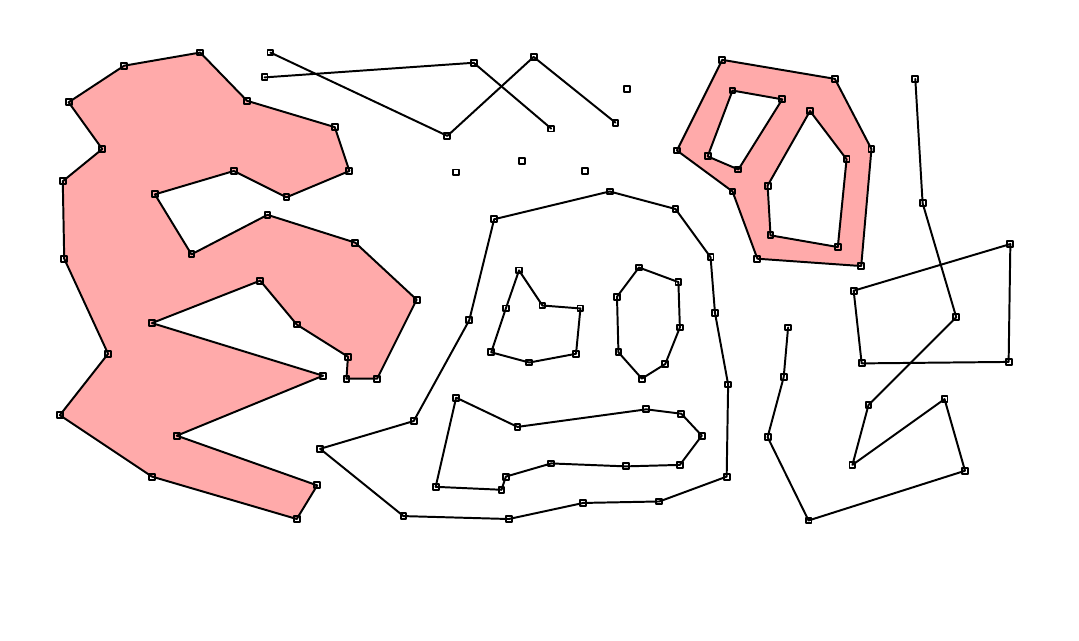
\begin{tikzpicture}[scale=13.0]
\clip (0,0) rectangle (1.000000,-0.571429);
\definecolor{FFFFFF}{rgb}{1.00000,1.00000,1.00000}
\definecolor{FFAAAA}{rgb}{1.00000,0.66667,0.66667}
\definecolor{000000}{rgb}{0.00000,0.00000,0.00000}
\clip (0,0) rectangle (1,-1);
\fill[color=FFFFFF] (0.00000, 0.00000) rectangle (1.00000, -0.57143);
\fill[color=FFAAAA, even odd rule] (0.09429,-0.03714) -- (0.04000,-0.07286) -- (0.07286,-0.11857) -- (0.03429,-0.15000) -- (0.03571,-0.22571) -- (0.07857,-0.31857) -- (0.03143,-0.37857) -- (0.12143,-0.43857) -- (0.26286,-0.48000) -- (0.28286,-0.44714) -- (0.14571,-0.39857) -- (0.28857,-0.34000) -- (0.12143,-0.28857) -- (0.22714,-0.24714) -- (0.26286,-0.29000) -- (0.31286,-0.32143) -- (0.31143,-0.34286) -- (0.34143,-0.34286) -- (0.38000,-0.26571) -- (0.32000,-0.21000) -- (0.23429,-0.18286) -- (0.16000,-0.22143) -- (0.12429,-0.16286) -- (0.20143,-0.14000) -- (0.25286,-0.16571) -- (0.31429,-0.14000) -- (0.30000,-0.09714) -- (0.21429,-0.07143) -- (0.16857,-0.02429) -- cycle;
\fill[color=FFAAAA, even odd rule] (0.67857,-0.03143) -- (0.63429,-0.12000) -- (0.68857,-0.16000) -- (0.71286,-0.22571) -- (0.81429,-0.23286) -- (0.82429,-0.11857) -- (0.78857,-0.05000) -- cycle (0.76429,-0.08143) -- (0.72286,-0.15429) -- (0.72571,-0.20286) -- (0.79143,-0.21429) -- (0.80000,-0.12857) -- cycle (0.68857,-0.06143) -- (0.66429,-0.12571) -- (0.69429,-0.13857) -- (0.73714,-0.07000) -- cycle;
\draw[line width=0.25000mm, join=round, cap=round, color=000000] (0.23143,-0.04857) -- (0.43571,-0.03429) -- (0.51143,-0.09857);
\draw[line width=0.25000mm, join=round, cap=round, color=000000] (0.23714,-0.02429) -- (0.41000,-0.10571) -- (0.49429,-0.02857) -- (0.57429,-0.09286);
\draw[line width=0.25000mm, join=round, cap=round, color=000000] (0.95831,-0.32654) -- (0.81475,-0.32797) -- (0.80693,-0.25697) -- (0.96000,-0.21137) -- cycle;
\draw[line width=0.25000mm, join=round, cap=round, color=000000] (0.50286,-0.27143) -- (0.48000,-0.23714) -- (0.46714,-0.27429) -- (0.45286,-0.31714) -- (0.49000,-0.32714) -- (0.53571,-0.31857) -- (0.54000,-0.27429) -- cycle;
\draw[line width=0.25000mm, join=round, cap=round, color=000000] (0.59714,-0.23429) -- (0.57571,-0.26286) -- (0.57714,-0.31714) -- (0.60000,-0.34286) -- (0.62286,-0.32857) -- (0.63714,-0.29286) -- (0.63571,-0.24857) -- cycle;
\draw[line width=0.25000mm, join=round, cap=round, color=000000] (0.60429,-0.37286) -- (0.47857,-0.39000) -- (0.41857,-0.36143) -- (0.39857,-0.44857) -- (0.46286,-0.45143) -- (0.46714,-0.43857) -- (0.51143,-0.42571) -- (0.58429,-0.42857) -- (0.63714,-0.42714) -- (0.65857,-0.39857) -- (0.63857,-0.37714) -- cycle;
\draw[line width=0.25000mm, join=round, cap=round, color=000000] (0.56857,-0.16000) -- (0.45571,-0.18714) -- (0.43143,-0.28571) -- (0.37714,-0.38429) -- (0.28571,-0.41143) -- (0.36714,-0.47714) -- (0.47000,-0.48000) -- (0.54286,-0.46429) -- (0.61714,-0.46286) -- (0.68286,-0.43857) -- (0.68429,-0.34857) -- (0.67143,-0.27857) -- (0.66714,-0.22429) -- (0.63286,-0.17714) -- cycle;
\draw[line width=0.25000mm, join=round, cap=round, color=000000] (0.74286,-0.29286) -- (0.73857,-0.34143) -- (0.72286,-0.40000) -- (0.76286,-0.48143) -- (0.91571,-0.43286) -- (0.89571,-0.36286) -- (0.80571,-0.42714) -- (0.82143,-0.36857) -- (0.90714,-0.28286) -- (0.87429,-0.17143) -- (0.86714,-0.05000);
\draw[line width=0.25000mm, join=round, cap=round, color=000000] (0.09429,-0.03714) -- (0.04000,-0.07286) -- (0.07286,-0.11857) -- (0.03429,-0.15000) -- (0.03571,-0.22571) -- (0.07857,-0.31857) -- (0.03143,-0.37857) -- (0.12143,-0.43857) -- (0.26286,-0.48000) -- (0.28286,-0.44714) -- (0.14571,-0.39857) -- (0.28857,-0.34000) -- (0.12143,-0.28857) -- (0.22714,-0.24714) -- (0.26286,-0.29000) -- (0.31286,-0.32143) -- (0.31143,-0.34286) -- (0.34143,-0.34286) -- (0.38000,-0.26571) -- (0.32000,-0.21000) -- (0.23429,-0.18286) -- (0.16000,-0.22143) -- (0.12429,-0.16286) -- (0.20143,-0.14000) -- (0.25286,-0.16571) -- (0.31429,-0.14000) -- (0.30000,-0.09714) -- (0.21429,-0.07143) -- (0.16857,-0.02429) -- cycle;
\draw[line width=0.25000mm, join=round, cap=round, color=000000] (0.67857,-0.03143) -- (0.63429,-0.12000) -- (0.68857,-0.16000) -- (0.71286,-0.22571) -- (0.81429,-0.23286) -- (0.82429,-0.11857) -- (0.78857,-0.05000) -- cycle;
\draw[line width=0.25000mm, join=round, cap=round, color=000000] (0.76429,-0.08143) -- (0.72286,-0.15429) -- (0.72571,-0.20286) -- (0.79143,-0.21429) -- (0.80000,-0.12857) -- cycle;
\draw[line width=0.25000mm, join=round, cap=round, color=000000] (0.68857,-0.06143) -- (0.66429,-0.12571) -- (0.69429,-0.13857) -- (0.73714,-0.07000) -- cycle;
\draw[line width=0.25000mm, join=round, cap=round, color=000000] (0.22857, -0.04571) rectangle (0.23429, -0.05143);
\draw[line width=0.25000mm, join=round, cap=round, color=000000] (0.43286, -0.03143) rectangle (0.43857, -0.03714);
\draw[line width=0.25000mm, join=round, cap=round, color=000000] (0.50857, -0.09571) rectangle (0.51429, -0.10143);
\draw[line width=0.25000mm, join=round, cap=round, color=000000] (0.23429, -0.02143) rectangle (0.24000, -0.02714);
\draw[line width=0.25000mm, join=round, cap=round, color=000000] (0.40714, -0.10286) rectangle (0.41286, -0.10857);
\draw[line width=0.25000mm, join=round, cap=round, color=000000] (0.49143, -0.02571) rectangle (0.49714, -0.03143);
\draw[line width=0.25000mm, join=round, cap=round, color=000000] (0.57143, -0.09000) rectangle (0.57714, -0.09571);
\draw[line width=0.25000mm, join=round, cap=round, color=000000] (0.95546, -0.32368) rectangle (0.96117, -0.32939);
\draw[line width=0.25000mm, join=round, cap=round, color=000000] (0.81189, -0.32511) rectangle (0.81761, -0.33083);
\draw[line width=0.25000mm, join=round, cap=round, color=000000] (0.80408, -0.25412) rectangle (0.80979, -0.25983);
\draw[line width=0.25000mm, join=round, cap=round, color=000000] (0.95715, -0.20852) rectangle (0.96286, -0.21423);
\draw[line width=0.25000mm, join=round, cap=round, color=000000] (0.41571, -0.13857) rectangle (0.42143, -0.14429);
\draw[line width=0.25000mm, join=round, cap=round, color=000000] (0.48000, -0.12714) rectangle (0.48571, -0.13286);
\draw[line width=0.25000mm, join=round, cap=round, color=000000] (0.54143, -0.13714) rectangle (0.54714, -0.14286);
\draw[line width=0.25000mm, join=round, cap=round, color=000000] (0.58286, -0.05714) rectangle (0.58857, -0.06286);
\draw[line width=0.25000mm, join=round, cap=round, color=000000] (0.50000, -0.26857) rectangle (0.50571, -0.27429);
\draw[line width=0.25000mm, join=round, cap=round, color=000000] (0.47714, -0.23429) rectangle (0.48286, -0.24000);
\draw[line width=0.25000mm, join=round, cap=round, color=000000] (0.46429, -0.27143) rectangle (0.47000, -0.27714);
\draw[line width=0.25000mm, join=round, cap=round, color=000000] (0.45000, -0.31429) rectangle (0.45571, -0.32000);
\draw[line width=0.25000mm, join=round, cap=round, color=000000] (0.48714, -0.32429) rectangle (0.49286, -0.33000);
\draw[line width=0.25000mm, join=round, cap=round, color=000000] (0.53286, -0.31571) rectangle (0.53857, -0.32143);
\draw[line width=0.25000mm, join=round, cap=round, color=000000] (0.53714, -0.27143) rectangle (0.54286, -0.27714);
\draw[line width=0.25000mm, join=round, cap=round, color=000000] (0.59429, -0.23143) rectangle (0.60000, -0.23714);
\draw[line width=0.25000mm, join=round, cap=round, color=000000] (0.57286, -0.26000) rectangle (0.57857, -0.26571);
\draw[line width=0.25000mm, join=round, cap=round, color=000000] (0.57429, -0.31429) rectangle (0.58000, -0.32000);
\draw[line width=0.25000mm, join=round, cap=round, color=000000] (0.59714, -0.34000) rectangle (0.60286, -0.34571);
\draw[line width=0.25000mm, join=round, cap=round, color=000000] (0.62000, -0.32571) rectangle (0.62571, -0.33143);
\draw[line width=0.25000mm, join=round, cap=round, color=000000] (0.63429, -0.29000) rectangle (0.64000, -0.29571);
\draw[line width=0.25000mm, join=round, cap=round, color=000000] (0.63286, -0.24571) rectangle (0.63857, -0.25143);
\draw[line width=0.25000mm, join=round, cap=round, color=000000] (0.60143, -0.37000) rectangle (0.60714, -0.37571);
\draw[line width=0.25000mm, join=round, cap=round, color=000000] (0.47571, -0.38714) rectangle (0.48143, -0.39286);
\draw[line width=0.25000mm, join=round, cap=round, color=000000] (0.41571, -0.35857) rectangle (0.42143, -0.36429);
\draw[line width=0.25000mm, join=round, cap=round, color=000000] (0.39571, -0.44571) rectangle (0.40143, -0.45143);
\draw[line width=0.25000mm, join=round, cap=round, color=000000] (0.46000, -0.44857) rectangle (0.46571, -0.45429);
\draw[line width=0.25000mm, join=round, cap=round, color=000000] (0.46429, -0.43571) rectangle (0.47000, -0.44143);
\draw[line width=0.25000mm, join=round, cap=round, color=000000] (0.50857, -0.42286) rectangle (0.51429, -0.42857);
\draw[line width=0.25000mm, join=round, cap=round, color=000000] (0.58143, -0.42571) rectangle (0.58714, -0.43143);
\draw[line width=0.25000mm, join=round, cap=round, color=000000] (0.63429, -0.42429) rectangle (0.64000, -0.43000);
\draw[line width=0.25000mm, join=round, cap=round, color=000000] (0.65571, -0.39571) rectangle (0.66143, -0.40143);
\draw[line width=0.25000mm, join=round, cap=round, color=000000] (0.63571, -0.37429) rectangle (0.64143, -0.38000);
\draw[line width=0.25000mm, join=round, cap=round, color=000000] (0.56571, -0.15714) rectangle (0.57143, -0.16286);
\draw[line width=0.25000mm, join=round, cap=round, color=000000] (0.45286, -0.18429) rectangle (0.45857, -0.19000);
\draw[line width=0.25000mm, join=round, cap=round, color=000000] (0.42857, -0.28286) rectangle (0.43429, -0.28857);
\draw[line width=0.25000mm, join=round, cap=round, color=000000] (0.37429, -0.38143) rectangle (0.38000, -0.38714);
\draw[line width=0.25000mm, join=round, cap=round, color=000000] (0.28286, -0.40857) rectangle (0.28857, -0.41429);
\draw[line width=0.25000mm, join=round, cap=round, color=000000] (0.36429, -0.47429) rectangle (0.37000, -0.48000);
\draw[line width=0.25000mm, join=round, cap=round, color=000000] (0.46714, -0.47714) rectangle (0.47286, -0.48286);
\draw[line width=0.25000mm, join=round, cap=round, color=000000] (0.54000, -0.46143) rectangle (0.54571, -0.46714);
\draw[line width=0.25000mm, join=round, cap=round, color=000000] (0.61429, -0.46000) rectangle (0.62000, -0.46571);
\draw[line width=0.25000mm, join=round, cap=round, color=000000] (0.68000, -0.43571) rectangle (0.68571, -0.44143);
\draw[line width=0.25000mm, join=round, cap=round, color=000000] (0.68143, -0.34571) rectangle (0.68714, -0.35143);
\draw[line width=0.25000mm, join=round, cap=round, color=000000] (0.66857, -0.27571) rectangle (0.67429, -0.28143);
\draw[line width=0.25000mm, join=round, cap=round, color=000000] (0.66429, -0.22143) rectangle (0.67000, -0.22714);
\draw[line width=0.25000mm, join=round, cap=round, color=000000] (0.63000, -0.17429) rectangle (0.63571, -0.18000);
\draw[line width=0.25000mm, join=round, cap=round, color=000000] (0.74000, -0.29000) rectangle (0.74571, -0.29571);
\draw[line width=0.25000mm, join=round, cap=round, color=000000] (0.73571, -0.33857) rectangle (0.74143, -0.34429);
\draw[line width=0.25000mm, join=round, cap=round, color=000000] (0.72000, -0.39714) rectangle (0.72571, -0.40286);
\draw[line width=0.25000mm, join=round, cap=round, color=000000] (0.76000, -0.47857) rectangle (0.76571, -0.48429);
\draw[line width=0.25000mm, join=round, cap=round, color=000000] (0.91286, -0.43000) rectangle (0.91857, -0.43571);
\draw[line width=0.25000mm, join=round, cap=round, color=000000] (0.89286, -0.36000) rectangle (0.89857, -0.36571);
\draw[line width=0.25000mm, join=round, cap=round, color=000000] (0.80286, -0.42429) rectangle (0.80857, -0.43000);
\draw[line width=0.25000mm, join=round, cap=round, color=000000] (0.81857, -0.36571) rectangle (0.82429, -0.37143);
\draw[line width=0.25000mm, join=round, cap=round, color=000000] (0.90429, -0.28000) rectangle (0.91000, -0.28571);
\draw[line width=0.25000mm, join=round, cap=round, color=000000] (0.87143, -0.16857) rectangle (0.87714, -0.17429);
\draw[line width=0.25000mm, join=round, cap=round, color=000000] (0.86429, -0.04714) rectangle (0.87000, -0.05286);
\draw[line width=0.25000mm, join=round, cap=round, color=000000] (0.09143, -0.03429) rectangle (0.09714, -0.04000);
\draw[line width=0.25000mm, join=round, cap=round, color=000000] (0.03714, -0.07000) rectangle (0.04286, -0.07571);
\draw[line width=0.25000mm, join=round, cap=round, color=000000] (0.07000, -0.11571) rectangle (0.07571, -0.12143);
\draw[line width=0.25000mm, join=round, cap=round, color=000000] (0.03143, -0.14714) rectangle (0.03714, -0.15286);
\draw[line width=0.25000mm, join=round, cap=round, color=000000] (0.03286, -0.22286) rectangle (0.03857, -0.22857);
\draw[line width=0.25000mm, join=round, cap=round, color=000000] (0.07571, -0.31571) rectangle (0.08143, -0.32143);
\draw[line width=0.25000mm, join=round, cap=round, color=000000] (0.02857, -0.37571) rectangle (0.03429, -0.38143);
\draw[line width=0.25000mm, join=round, cap=round, color=000000] (0.11857, -0.43571) rectangle (0.12429, -0.44143);
\draw[line width=0.25000mm, join=round, cap=round, color=000000] (0.26000, -0.47714) rectangle (0.26571, -0.48286);
\draw[line width=0.25000mm, join=round, cap=round, color=000000] (0.28000, -0.44429) rectangle (0.28571, -0.45000);
\draw[line width=0.25000mm, join=round, cap=round, color=000000] (0.14286, -0.39571) rectangle (0.14857, -0.40143);
\draw[line width=0.25000mm, join=round, cap=round, color=000000] (0.28571, -0.33714) rectangle (0.29143, -0.34286);
\draw[line width=0.25000mm, join=round, cap=round, color=000000] (0.11857, -0.28571) rectangle (0.12429, -0.29143);
\draw[line width=0.25000mm, join=round, cap=round, color=000000] (0.22429, -0.24429) rectangle (0.23000, -0.25000);
\draw[line width=0.25000mm, join=round, cap=round, color=000000] (0.26000, -0.28714) rectangle (0.26571, -0.29286);
\draw[line width=0.25000mm, join=round, cap=round, color=000000] (0.31000, -0.31857) rectangle (0.31571, -0.32429);
\draw[line width=0.25000mm, join=round, cap=round, color=000000] (0.30857, -0.34000) rectangle (0.31429, -0.34571);
\draw[line width=0.25000mm, join=round, cap=round, color=000000] (0.33857, -0.34000) rectangle (0.34429, -0.34571);
\draw[line width=0.25000mm, join=round, cap=round, color=000000] (0.37714, -0.26286) rectangle (0.38286, -0.26857);
\draw[line width=0.25000mm, join=round, cap=round, color=000000] (0.31714, -0.20714) rectangle (0.32286, -0.21286);
\draw[line width=0.25000mm, join=round, cap=round, color=000000] (0.23143, -0.18000) rectangle (0.23714, -0.18571);
\draw[line width=0.25000mm, join=round, cap=round, color=000000] (0.15714, -0.21857) rectangle (0.16286, -0.22429);
\draw[line width=0.25000mm, join=round, cap=round, color=000000] (0.12143, -0.16000) rectangle (0.12714, -0.16571);
\draw[line width=0.25000mm, join=round, cap=round, color=000000] (0.19857, -0.13714) rectangle (0.20429, -0.14286);
\draw[line width=0.25000mm, join=round, cap=round, color=000000] (0.25000, -0.16286) rectangle (0.25571, -0.16857);
\draw[line width=0.25000mm, join=round, cap=round, color=000000] (0.31143, -0.13714) rectangle (0.31714, -0.14286);
\draw[line width=0.25000mm, join=round, cap=round, color=000000] (0.29714, -0.09429) rectangle (0.30286, -0.10000);
\draw[line width=0.25000mm, join=round, cap=round, color=000000] (0.21143, -0.06857) rectangle (0.21714, -0.07429);
\draw[line width=0.25000mm, join=round, cap=round, color=000000] (0.16571, -0.02143) rectangle (0.17143, -0.02714);
\draw[line width=0.25000mm, join=round, cap=round, color=000000] (0.67571, -0.02857) rectangle (0.68143, -0.03429);
\draw[line width=0.25000mm, join=round, cap=round, color=000000] (0.63143, -0.11714) rectangle (0.63714, -0.12286);
\draw[line width=0.25000mm, join=round, cap=round, color=000000] (0.68571, -0.15714) rectangle (0.69143, -0.16286);
\draw[line width=0.25000mm, join=round, cap=round, color=000000] (0.71000, -0.22286) rectangle (0.71571, -0.22857);
\draw[line width=0.25000mm, join=round, cap=round, color=000000] (0.81143, -0.23000) rectangle (0.81714, -0.23571);
\draw[line width=0.25000mm, join=round, cap=round, color=000000] (0.82143, -0.11571) rectangle (0.82714, -0.12143);
\draw[line width=0.25000mm, join=round, cap=round, color=000000] (0.78571, -0.04714) rectangle (0.79143, -0.05286);
\draw[line width=0.25000mm, join=round, cap=round, color=000000] (0.76143, -0.07857) rectangle (0.76714, -0.08429);
\draw[line width=0.25000mm, join=round, cap=round, color=000000] (0.72000, -0.15143) rectangle (0.72571, -0.15714);
\draw[line width=0.25000mm, join=round, cap=round, color=000000] (0.72286, -0.20000) rectangle (0.72857, -0.20571);
\draw[line width=0.25000mm, join=round, cap=round, color=000000] (0.78857, -0.21143) rectangle (0.79429, -0.21714);
\draw[line width=0.25000mm, join=round, cap=round, color=000000] (0.79714, -0.12571) rectangle (0.80286, -0.13143);
\draw[line width=0.25000mm, join=round, cap=round, color=000000] (0.68571, -0.05857) rectangle (0.69143, -0.06429);
\draw[line width=0.25000mm, join=round, cap=round, color=000000] (0.66143, -0.12286) rectangle (0.66714, -0.12857);
\draw[line width=0.25000mm, join=round, cap=round, color=000000] (0.69143, -0.13571) rectangle (0.69714, -0.14143);
\draw[line width=0.25000mm, join=round, cap=round, color=000000] (0.73429, -0.06714) rectangle (0.74000, -0.07286);
\end{tikzpicture}
\end{center}
Also there should be some text below. This text block
should also be a not too short, so that there will be a line
break within the paragraph.
\begin{center}
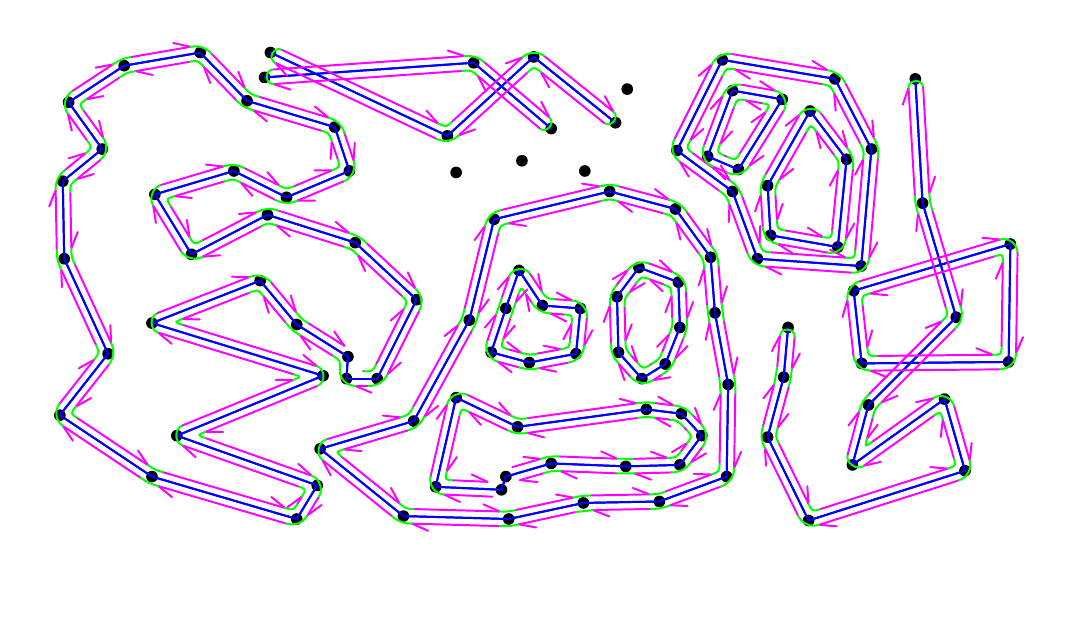
\begin{tikzpicture}[scale=13.0]
\clip (0,0) rectangle (1.000000,-0.571429);
\definecolor{FFFFFF}{rgb}{1.00000,1.00000,1.00000}
\definecolor{000000}{rgb}{0.00000,0.00000,0.00000}
\definecolor{0000FF}{rgb}{0.00000,0.00000,1.00000}
\definecolor{FF00FF}{rgb}{1.00000,0.00000,1.00000}
\definecolor{00FF00}{rgb}{0.00000,1.00000,0.00000}
\clip (0,0) rectangle (1,-1);
\fill[color=FFFFFF] (0.00000, 0.00000) rectangle (1.00000, -0.57143);
\fill[color=000000] (0.23143,-0.04857) circle (0.00571);
\fill[color=000000] (0.43571,-0.03429) circle (0.00571);
\fill[color=000000] (0.51143,-0.09857) circle (0.00571);
\fill[color=000000] (0.23714,-0.02429) circle (0.00571);
\fill[color=000000] (0.41000,-0.10571) circle (0.00571);
\fill[color=000000] (0.49429,-0.02857) circle (0.00571);
\fill[color=000000] (0.57429,-0.09286) circle (0.00571);
\fill[color=000000] (0.95831,-0.32654) circle (0.00571);
\fill[color=000000] (0.81475,-0.32797) circle (0.00571);
\fill[color=000000] (0.80693,-0.25697) circle (0.00571);
\fill[color=000000] (0.96000,-0.21137) circle (0.00571);
\fill[color=000000] (0.41857,-0.14143) circle (0.00571);
\fill[color=000000] (0.48286,-0.13000) circle (0.00571);
\fill[color=000000] (0.54429,-0.14000) circle (0.00571);
\fill[color=000000] (0.58571,-0.06000) circle (0.00571);
\fill[color=000000] (0.50286,-0.27143) circle (0.00571);
\fill[color=000000] (0.48000,-0.23714) circle (0.00571);
\fill[color=000000] (0.46714,-0.27429) circle (0.00571);
\fill[color=000000] (0.45286,-0.31714) circle (0.00571);
\fill[color=000000] (0.49000,-0.32714) circle (0.00571);
\fill[color=000000] (0.53571,-0.31857) circle (0.00571);
\fill[color=000000] (0.54000,-0.27429) circle (0.00571);
\fill[color=000000] (0.59714,-0.23429) circle (0.00571);
\fill[color=000000] (0.57571,-0.26286) circle (0.00571);
\fill[color=000000] (0.57714,-0.31714) circle (0.00571);
\fill[color=000000] (0.60000,-0.34286) circle (0.00571);
\fill[color=000000] (0.62286,-0.32857) circle (0.00571);
\fill[color=000000] (0.63714,-0.29286) circle (0.00571);
\fill[color=000000] (0.63571,-0.24857) circle (0.00571);
\fill[color=000000] (0.60429,-0.37286) circle (0.00571);
\fill[color=000000] (0.47857,-0.39000) circle (0.00571);
\fill[color=000000] (0.41857,-0.36143) circle (0.00571);
\fill[color=000000] (0.39857,-0.44857) circle (0.00571);
\fill[color=000000] (0.46286,-0.45143) circle (0.00571);
\fill[color=000000] (0.46714,-0.43857) circle (0.00571);
\fill[color=000000] (0.51143,-0.42571) circle (0.00571);
\fill[color=000000] (0.58429,-0.42857) circle (0.00571);
\fill[color=000000] (0.63714,-0.42714) circle (0.00571);
\fill[color=000000] (0.65857,-0.39857) circle (0.00571);
\fill[color=000000] (0.63857,-0.37714) circle (0.00571);
\fill[color=000000] (0.56857,-0.16000) circle (0.00571);
\fill[color=000000] (0.45571,-0.18714) circle (0.00571);
\fill[color=000000] (0.43143,-0.28571) circle (0.00571);
\fill[color=000000] (0.37714,-0.38429) circle (0.00571);
\fill[color=000000] (0.28571,-0.41143) circle (0.00571);
\fill[color=000000] (0.36714,-0.47714) circle (0.00571);
\fill[color=000000] (0.47000,-0.48000) circle (0.00571);
\fill[color=000000] (0.54286,-0.46429) circle (0.00571);
\fill[color=000000] (0.61714,-0.46286) circle (0.00571);
\fill[color=000000] (0.68286,-0.43857) circle (0.00571);
\fill[color=000000] (0.68429,-0.34857) circle (0.00571);
\fill[color=000000] (0.67143,-0.27857) circle (0.00571);
\fill[color=000000] (0.66714,-0.22429) circle (0.00571);
\fill[color=000000] (0.63286,-0.17714) circle (0.00571);
\fill[color=000000] (0.74286,-0.29286) circle (0.00571);
\fill[color=000000] (0.73857,-0.34143) circle (0.00571);
\fill[color=000000] (0.72286,-0.40000) circle (0.00571);
\fill[color=000000] (0.76286,-0.48143) circle (0.00571);
\fill[color=000000] (0.91571,-0.43286) circle (0.00571);
\fill[color=000000] (0.89571,-0.36286) circle (0.00571);
\fill[color=000000] (0.80571,-0.42714) circle (0.00571);
\fill[color=000000] (0.82143,-0.36857) circle (0.00571);
\fill[color=000000] (0.90714,-0.28286) circle (0.00571);
\fill[color=000000] (0.87429,-0.17143) circle (0.00571);
\fill[color=000000] (0.86714,-0.05000) circle (0.00571);
\fill[color=000000] (0.09429,-0.03714) circle (0.00571);
\fill[color=000000] (0.04000,-0.07286) circle (0.00571);
\fill[color=000000] (0.07286,-0.11857) circle (0.00571);
\fill[color=000000] (0.03429,-0.15000) circle (0.00571);
\fill[color=000000] (0.03571,-0.22571) circle (0.00571);
\fill[color=000000] (0.07857,-0.31857) circle (0.00571);
\fill[color=000000] (0.03143,-0.37857) circle (0.00571);
\fill[color=000000] (0.12143,-0.43857) circle (0.00571);
\fill[color=000000] (0.26286,-0.48000) circle (0.00571);
\fill[color=000000] (0.28286,-0.44714) circle (0.00571);
\fill[color=000000] (0.14571,-0.39857) circle (0.00571);
\fill[color=000000] (0.28857,-0.34000) circle (0.00571);
\fill[color=000000] (0.12143,-0.28857) circle (0.00571);
\fill[color=000000] (0.22714,-0.24714) circle (0.00571);
\fill[color=000000] (0.26286,-0.29000) circle (0.00571);
\fill[color=000000] (0.31286,-0.32143) circle (0.00571);
\fill[color=000000] (0.31143,-0.34286) circle (0.00571);
\fill[color=000000] (0.34143,-0.34286) circle (0.00571);
\fill[color=000000] (0.38000,-0.26571) circle (0.00571);
\fill[color=000000] (0.32000,-0.21000) circle (0.00571);
\fill[color=000000] (0.23429,-0.18286) circle (0.00571);
\fill[color=000000] (0.16000,-0.22143) circle (0.00571);
\fill[color=000000] (0.12429,-0.16286) circle (0.00571);
\fill[color=000000] (0.20143,-0.14000) circle (0.00571);
\fill[color=000000] (0.25286,-0.16571) circle (0.00571);
\fill[color=000000] (0.31429,-0.14000) circle (0.00571);
\fill[color=000000] (0.30000,-0.09714) circle (0.00571);
\fill[color=000000] (0.21429,-0.07143) circle (0.00571);
\fill[color=000000] (0.16857,-0.02429) circle (0.00571);
\fill[color=000000] (0.67857,-0.03143) circle (0.00571);
\fill[color=000000] (0.63429,-0.12000) circle (0.00571);
\fill[color=000000] (0.68857,-0.16000) circle (0.00571);
\fill[color=000000] (0.71286,-0.22571) circle (0.00571);
\fill[color=000000] (0.81429,-0.23286) circle (0.00571);
\fill[color=000000] (0.82429,-0.11857) circle (0.00571);
\fill[color=000000] (0.78857,-0.05000) circle (0.00571);
\fill[color=000000] (0.76429,-0.08143) circle (0.00571);
\fill[color=000000] (0.72286,-0.15429) circle (0.00571);
\fill[color=000000] (0.72571,-0.20286) circle (0.00571);
\fill[color=000000] (0.79143,-0.21429) circle (0.00571);
\fill[color=000000] (0.80000,-0.12857) circle (0.00571);
\fill[color=000000] (0.68857,-0.06143) circle (0.00571);
\fill[color=000000] (0.66429,-0.12571) circle (0.00571);
\fill[color=000000] (0.69429,-0.13857) circle (0.00571);
\fill[color=000000] (0.73714,-0.07000) circle (0.00571);
\draw[line width=0.25000mm, join=round, cap=round, color=0000FF] (0.23143,-0.04857) -- (0.43571,-0.03429);
\draw[line width=0.25000mm, join=round, cap=round, color=0000FF] (0.43571,-0.03429) -- (0.23143,-0.04857);
\draw[line width=0.25000mm, join=round, cap=round, color=0000FF] (0.43571,-0.03429) -- (0.51143,-0.09857);
\draw[line width=0.25000mm, join=round, cap=round, color=0000FF] (0.51143,-0.09857) -- (0.43571,-0.03429);
\draw[line width=0.25000mm, join=round, cap=round, color=0000FF] (0.23714,-0.02429) -- (0.41000,-0.10571);
\draw[line width=0.25000mm, join=round, cap=round, color=0000FF] (0.41000,-0.10571) -- (0.23714,-0.02429);
\draw[line width=0.25000mm, join=round, cap=round, color=0000FF] (0.41000,-0.10571) -- (0.49429,-0.02857);
\draw[line width=0.25000mm, join=round, cap=round, color=0000FF] (0.49429,-0.02857) -- (0.41000,-0.10571);
\draw[line width=0.25000mm, join=round, cap=round, color=0000FF] (0.49429,-0.02857) -- (0.57429,-0.09286);
\draw[line width=0.25000mm, join=round, cap=round, color=0000FF] (0.57429,-0.09286) -- (0.49429,-0.02857);
\draw[line width=0.25000mm, join=round, cap=round, color=0000FF] (0.95831,-0.32654) -- (0.81475,-0.32797);
\draw[line width=0.25000mm, join=round, cap=round, color=0000FF] (0.81475,-0.32797) -- (0.95831,-0.32654);
\draw[line width=0.25000mm, join=round, cap=round, color=0000FF] (0.81475,-0.32797) -- (0.80693,-0.25697);
\draw[line width=0.25000mm, join=round, cap=round, color=0000FF] (0.80693,-0.25697) -- (0.81475,-0.32797);
\draw[line width=0.25000mm, join=round, cap=round, color=0000FF] (0.80693,-0.25697) -- (0.96000,-0.21137);
\draw[line width=0.25000mm, join=round, cap=round, color=0000FF] (0.96000,-0.21137) -- (0.80693,-0.25697);
\draw[line width=0.25000mm, join=round, cap=round, color=0000FF] (0.96000,-0.21137) -- (0.95831,-0.32654);
\draw[line width=0.25000mm, join=round, cap=round, color=0000FF] (0.95831,-0.32654) -- (0.96000,-0.21137);
\draw[line width=0.25000mm, join=round, cap=round, color=0000FF] (0.50286,-0.27143) -- (0.48000,-0.23714);
\draw[line width=0.25000mm, join=round, cap=round, color=0000FF] (0.48000,-0.23714) -- (0.50286,-0.27143);
\draw[line width=0.25000mm, join=round, cap=round, color=0000FF] (0.48000,-0.23714) -- (0.46714,-0.27429);
\draw[line width=0.25000mm, join=round, cap=round, color=0000FF] (0.46714,-0.27429) -- (0.48000,-0.23714);
\draw[line width=0.25000mm, join=round, cap=round, color=0000FF] (0.46714,-0.27429) -- (0.45286,-0.31714);
\draw[line width=0.25000mm, join=round, cap=round, color=0000FF] (0.45286,-0.31714) -- (0.46714,-0.27429);
\draw[line width=0.25000mm, join=round, cap=round, color=0000FF] (0.45286,-0.31714) -- (0.49000,-0.32714);
\draw[line width=0.25000mm, join=round, cap=round, color=0000FF] (0.49000,-0.32714) -- (0.45286,-0.31714);
\draw[line width=0.25000mm, join=round, cap=round, color=0000FF] (0.49000,-0.32714) -- (0.53571,-0.31857);
\draw[line width=0.25000mm, join=round, cap=round, color=0000FF] (0.53571,-0.31857) -- (0.49000,-0.32714);
\draw[line width=0.25000mm, join=round, cap=round, color=0000FF] (0.53571,-0.31857) -- (0.54000,-0.27429);
\draw[line width=0.25000mm, join=round, cap=round, color=0000FF] (0.54000,-0.27429) -- (0.53571,-0.31857);
\draw[line width=0.25000mm, join=round, cap=round, color=0000FF] (0.54000,-0.27429) -- (0.50286,-0.27143);
\draw[line width=0.25000mm, join=round, cap=round, color=0000FF] (0.50286,-0.27143) -- (0.54000,-0.27429);
\draw[line width=0.25000mm, join=round, cap=round, color=0000FF] (0.59714,-0.23429) -- (0.57571,-0.26286);
\draw[line width=0.25000mm, join=round, cap=round, color=0000FF] (0.57571,-0.26286) -- (0.59714,-0.23429);
\draw[line width=0.25000mm, join=round, cap=round, color=0000FF] (0.57571,-0.26286) -- (0.57714,-0.31714);
\draw[line width=0.25000mm, join=round, cap=round, color=0000FF] (0.57714,-0.31714) -- (0.57571,-0.26286);
\draw[line width=0.25000mm, join=round, cap=round, color=0000FF] (0.57714,-0.31714) -- (0.60000,-0.34286);
\draw[line width=0.25000mm, join=round, cap=round, color=0000FF] (0.60000,-0.34286) -- (0.57714,-0.31714);
\draw[line width=0.25000mm, join=round, cap=round, color=0000FF] (0.60000,-0.34286) -- (0.62286,-0.32857);
\draw[line width=0.25000mm, join=round, cap=round, color=0000FF] (0.62286,-0.32857) -- (0.60000,-0.34286);
\draw[line width=0.25000mm, join=round, cap=round, color=0000FF] (0.62286,-0.32857) -- (0.63714,-0.29286);
\draw[line width=0.25000mm, join=round, cap=round, color=0000FF] (0.63714,-0.29286) -- (0.62286,-0.32857);
\draw[line width=0.25000mm, join=round, cap=round, color=0000FF] (0.63714,-0.29286) -- (0.63571,-0.24857);
\draw[line width=0.25000mm, join=round, cap=round, color=0000FF] (0.63571,-0.24857) -- (0.63714,-0.29286);
\draw[line width=0.25000mm, join=round, cap=round, color=0000FF] (0.63571,-0.24857) -- (0.59714,-0.23429);
\draw[line width=0.25000mm, join=round, cap=round, color=0000FF] (0.59714,-0.23429) -- (0.63571,-0.24857);
\draw[line width=0.25000mm, join=round, cap=round, color=0000FF] (0.60429,-0.37286) -- (0.47857,-0.39000);
\draw[line width=0.25000mm, join=round, cap=round, color=0000FF] (0.47857,-0.39000) -- (0.60429,-0.37286);
\draw[line width=0.25000mm, join=round, cap=round, color=0000FF] (0.47857,-0.39000) -- (0.41857,-0.36143);
\draw[line width=0.25000mm, join=round, cap=round, color=0000FF] (0.41857,-0.36143) -- (0.47857,-0.39000);
\draw[line width=0.25000mm, join=round, cap=round, color=0000FF] (0.41857,-0.36143) -- (0.39857,-0.44857);
\draw[line width=0.25000mm, join=round, cap=round, color=0000FF] (0.39857,-0.44857) -- (0.41857,-0.36143);
\draw[line width=0.25000mm, join=round, cap=round, color=0000FF] (0.39857,-0.44857) -- (0.46286,-0.45143);
\draw[line width=0.25000mm, join=round, cap=round, color=0000FF] (0.46286,-0.45143) -- (0.39857,-0.44857);
\draw[line width=0.25000mm, join=round, cap=round, color=0000FF] (0.46286,-0.45143) -- (0.46714,-0.43857);
\draw[line width=0.25000mm, join=round, cap=round, color=0000FF] (0.46714,-0.43857) -- (0.46286,-0.45143);
\draw[line width=0.25000mm, join=round, cap=round, color=0000FF] (0.46714,-0.43857) -- (0.51143,-0.42571);
\draw[line width=0.25000mm, join=round, cap=round, color=0000FF] (0.51143,-0.42571) -- (0.46714,-0.43857);
\draw[line width=0.25000mm, join=round, cap=round, color=0000FF] (0.51143,-0.42571) -- (0.58429,-0.42857);
\draw[line width=0.25000mm, join=round, cap=round, color=0000FF] (0.58429,-0.42857) -- (0.51143,-0.42571);
\draw[line width=0.25000mm, join=round, cap=round, color=0000FF] (0.58429,-0.42857) -- (0.63714,-0.42714);
\draw[line width=0.25000mm, join=round, cap=round, color=0000FF] (0.63714,-0.42714) -- (0.58429,-0.42857);
\draw[line width=0.25000mm, join=round, cap=round, color=0000FF] (0.63714,-0.42714) -- (0.65857,-0.39857);
\draw[line width=0.25000mm, join=round, cap=round, color=0000FF] (0.65857,-0.39857) -- (0.63714,-0.42714);
\draw[line width=0.25000mm, join=round, cap=round, color=0000FF] (0.65857,-0.39857) -- (0.63857,-0.37714);
\draw[line width=0.25000mm, join=round, cap=round, color=0000FF] (0.63857,-0.37714) -- (0.65857,-0.39857);
\draw[line width=0.25000mm, join=round, cap=round, color=0000FF] (0.63857,-0.37714) -- (0.60429,-0.37286);
\draw[line width=0.25000mm, join=round, cap=round, color=0000FF] (0.60429,-0.37286) -- (0.63857,-0.37714);
\draw[line width=0.25000mm, join=round, cap=round, color=0000FF] (0.56857,-0.16000) -- (0.45571,-0.18714);
\draw[line width=0.25000mm, join=round, cap=round, color=0000FF] (0.45571,-0.18714) -- (0.56857,-0.16000);
\draw[line width=0.25000mm, join=round, cap=round, color=0000FF] (0.45571,-0.18714) -- (0.43143,-0.28571);
\draw[line width=0.25000mm, join=round, cap=round, color=0000FF] (0.43143,-0.28571) -- (0.45571,-0.18714);
\draw[line width=0.25000mm, join=round, cap=round, color=0000FF] (0.43143,-0.28571) -- (0.37714,-0.38429);
\draw[line width=0.25000mm, join=round, cap=round, color=0000FF] (0.37714,-0.38429) -- (0.43143,-0.28571);
\draw[line width=0.25000mm, join=round, cap=round, color=0000FF] (0.37714,-0.38429) -- (0.28571,-0.41143);
\draw[line width=0.25000mm, join=round, cap=round, color=0000FF] (0.28571,-0.41143) -- (0.37714,-0.38429);
\draw[line width=0.25000mm, join=round, cap=round, color=0000FF] (0.28571,-0.41143) -- (0.36714,-0.47714);
\draw[line width=0.25000mm, join=round, cap=round, color=0000FF] (0.36714,-0.47714) -- (0.28571,-0.41143);
\draw[line width=0.25000mm, join=round, cap=round, color=0000FF] (0.36714,-0.47714) -- (0.47000,-0.48000);
\draw[line width=0.25000mm, join=round, cap=round, color=0000FF] (0.47000,-0.48000) -- (0.36714,-0.47714);
\draw[line width=0.25000mm, join=round, cap=round, color=0000FF] (0.47000,-0.48000) -- (0.54286,-0.46429);
\draw[line width=0.25000mm, join=round, cap=round, color=0000FF] (0.54286,-0.46429) -- (0.47000,-0.48000);
\draw[line width=0.25000mm, join=round, cap=round, color=0000FF] (0.54286,-0.46429) -- (0.61714,-0.46286);
\draw[line width=0.25000mm, join=round, cap=round, color=0000FF] (0.61714,-0.46286) -- (0.54286,-0.46429);
\draw[line width=0.25000mm, join=round, cap=round, color=0000FF] (0.61714,-0.46286) -- (0.68286,-0.43857);
\draw[line width=0.25000mm, join=round, cap=round, color=0000FF] (0.68286,-0.43857) -- (0.61714,-0.46286);
\draw[line width=0.25000mm, join=round, cap=round, color=0000FF] (0.68286,-0.43857) -- (0.68429,-0.34857);
\draw[line width=0.25000mm, join=round, cap=round, color=0000FF] (0.68429,-0.34857) -- (0.68286,-0.43857);
\draw[line width=0.25000mm, join=round, cap=round, color=0000FF] (0.68429,-0.34857) -- (0.67143,-0.27857);
\draw[line width=0.25000mm, join=round, cap=round, color=0000FF] (0.67143,-0.27857) -- (0.68429,-0.34857);
\draw[line width=0.25000mm, join=round, cap=round, color=0000FF] (0.67143,-0.27857) -- (0.66714,-0.22429);
\draw[line width=0.25000mm, join=round, cap=round, color=0000FF] (0.66714,-0.22429) -- (0.67143,-0.27857);
\draw[line width=0.25000mm, join=round, cap=round, color=0000FF] (0.66714,-0.22429) -- (0.63286,-0.17714);
\draw[line width=0.25000mm, join=round, cap=round, color=0000FF] (0.63286,-0.17714) -- (0.66714,-0.22429);
\draw[line width=0.25000mm, join=round, cap=round, color=0000FF] (0.63286,-0.17714) -- (0.56857,-0.16000);
\draw[line width=0.25000mm, join=round, cap=round, color=0000FF] (0.56857,-0.16000) -- (0.63286,-0.17714);
\draw[line width=0.25000mm, join=round, cap=round, color=0000FF] (0.74286,-0.29286) -- (0.73857,-0.34143);
\draw[line width=0.25000mm, join=round, cap=round, color=0000FF] (0.73857,-0.34143) -- (0.74286,-0.29286);
\draw[line width=0.25000mm, join=round, cap=round, color=0000FF] (0.73857,-0.34143) -- (0.72286,-0.40000);
\draw[line width=0.25000mm, join=round, cap=round, color=0000FF] (0.72286,-0.40000) -- (0.73857,-0.34143);
\draw[line width=0.25000mm, join=round, cap=round, color=0000FF] (0.72286,-0.40000) -- (0.76286,-0.48143);
\draw[line width=0.25000mm, join=round, cap=round, color=0000FF] (0.76286,-0.48143) -- (0.72286,-0.40000);
\draw[line width=0.25000mm, join=round, cap=round, color=0000FF] (0.76286,-0.48143) -- (0.91571,-0.43286);
\draw[line width=0.25000mm, join=round, cap=round, color=0000FF] (0.91571,-0.43286) -- (0.76286,-0.48143);
\draw[line width=0.25000mm, join=round, cap=round, color=0000FF] (0.91571,-0.43286) -- (0.89571,-0.36286);
\draw[line width=0.25000mm, join=round, cap=round, color=0000FF] (0.89571,-0.36286) -- (0.91571,-0.43286);
\draw[line width=0.25000mm, join=round, cap=round, color=0000FF] (0.89571,-0.36286) -- (0.80571,-0.42714);
\draw[line width=0.25000mm, join=round, cap=round, color=0000FF] (0.80571,-0.42714) -- (0.89571,-0.36286);
\draw[line width=0.25000mm, join=round, cap=round, color=0000FF] (0.80571,-0.42714) -- (0.82143,-0.36857);
\draw[line width=0.25000mm, join=round, cap=round, color=0000FF] (0.82143,-0.36857) -- (0.80571,-0.42714);
\draw[line width=0.25000mm, join=round, cap=round, color=0000FF] (0.82143,-0.36857) -- (0.90714,-0.28286);
\draw[line width=0.25000mm, join=round, cap=round, color=0000FF] (0.90714,-0.28286) -- (0.82143,-0.36857);
\draw[line width=0.25000mm, join=round, cap=round, color=0000FF] (0.90714,-0.28286) -- (0.87429,-0.17143);
\draw[line width=0.25000mm, join=round, cap=round, color=0000FF] (0.87429,-0.17143) -- (0.90714,-0.28286);
\draw[line width=0.25000mm, join=round, cap=round, color=0000FF] (0.87429,-0.17143) -- (0.86714,-0.05000);
\draw[line width=0.25000mm, join=round, cap=round, color=0000FF] (0.86714,-0.05000) -- (0.87429,-0.17143);
\draw[line width=0.25000mm, join=round, cap=round, color=0000FF] (0.09429,-0.03714) -- (0.04000,-0.07286);
\draw[line width=0.25000mm, join=round, cap=round, color=0000FF] (0.04000,-0.07286) -- (0.09429,-0.03714);
\draw[line width=0.25000mm, join=round, cap=round, color=0000FF] (0.04000,-0.07286) -- (0.07286,-0.11857);
\draw[line width=0.25000mm, join=round, cap=round, color=0000FF] (0.07286,-0.11857) -- (0.04000,-0.07286);
\draw[line width=0.25000mm, join=round, cap=round, color=0000FF] (0.07286,-0.11857) -- (0.03429,-0.15000);
\draw[line width=0.25000mm, join=round, cap=round, color=0000FF] (0.03429,-0.15000) -- (0.07286,-0.11857);
\draw[line width=0.25000mm, join=round, cap=round, color=0000FF] (0.03429,-0.15000) -- (0.03571,-0.22571);
\draw[line width=0.25000mm, join=round, cap=round, color=0000FF] (0.03571,-0.22571) -- (0.03429,-0.15000);
\draw[line width=0.25000mm, join=round, cap=round, color=0000FF] (0.03571,-0.22571) -- (0.07857,-0.31857);
\draw[line width=0.25000mm, join=round, cap=round, color=0000FF] (0.07857,-0.31857) -- (0.03571,-0.22571);
\draw[line width=0.25000mm, join=round, cap=round, color=0000FF] (0.07857,-0.31857) -- (0.03143,-0.37857);
\draw[line width=0.25000mm, join=round, cap=round, color=0000FF] (0.03143,-0.37857) -- (0.07857,-0.31857);
\draw[line width=0.25000mm, join=round, cap=round, color=0000FF] (0.03143,-0.37857) -- (0.12143,-0.43857);
\draw[line width=0.25000mm, join=round, cap=round, color=0000FF] (0.12143,-0.43857) -- (0.03143,-0.37857);
\draw[line width=0.25000mm, join=round, cap=round, color=0000FF] (0.12143,-0.43857) -- (0.26286,-0.48000);
\draw[line width=0.25000mm, join=round, cap=round, color=0000FF] (0.26286,-0.48000) -- (0.12143,-0.43857);
\draw[line width=0.25000mm, join=round, cap=round, color=0000FF] (0.26286,-0.48000) -- (0.28286,-0.44714);
\draw[line width=0.25000mm, join=round, cap=round, color=0000FF] (0.28286,-0.44714) -- (0.26286,-0.48000);
\draw[line width=0.25000mm, join=round, cap=round, color=0000FF] (0.28286,-0.44714) -- (0.14571,-0.39857);
\draw[line width=0.25000mm, join=round, cap=round, color=0000FF] (0.14571,-0.39857) -- (0.28286,-0.44714);
\draw[line width=0.25000mm, join=round, cap=round, color=0000FF] (0.14571,-0.39857) -- (0.28857,-0.34000);
\draw[line width=0.25000mm, join=round, cap=round, color=0000FF] (0.28857,-0.34000) -- (0.14571,-0.39857);
\draw[line width=0.25000mm, join=round, cap=round, color=0000FF] (0.28857,-0.34000) -- (0.12143,-0.28857);
\draw[line width=0.25000mm, join=round, cap=round, color=0000FF] (0.12143,-0.28857) -- (0.28857,-0.34000);
\draw[line width=0.25000mm, join=round, cap=round, color=0000FF] (0.12143,-0.28857) -- (0.22714,-0.24714);
\draw[line width=0.25000mm, join=round, cap=round, color=0000FF] (0.22714,-0.24714) -- (0.12143,-0.28857);
\draw[line width=0.25000mm, join=round, cap=round, color=0000FF] (0.22714,-0.24714) -- (0.26286,-0.29000);
\draw[line width=0.25000mm, join=round, cap=round, color=0000FF] (0.26286,-0.29000) -- (0.22714,-0.24714);
\draw[line width=0.25000mm, join=round, cap=round, color=0000FF] (0.26286,-0.29000) -- (0.31286,-0.32143);
\draw[line width=0.25000mm, join=round, cap=round, color=0000FF] (0.31286,-0.32143) -- (0.26286,-0.29000);
\draw[line width=0.25000mm, join=round, cap=round, color=0000FF] (0.31286,-0.32143) -- (0.31143,-0.34286);
\draw[line width=0.25000mm, join=round, cap=round, color=0000FF] (0.31143,-0.34286) -- (0.31286,-0.32143);
\draw[line width=0.25000mm, join=round, cap=round, color=0000FF] (0.31143,-0.34286) -- (0.34143,-0.34286);
\draw[line width=0.25000mm, join=round, cap=round, color=0000FF] (0.34143,-0.34286) -- (0.31143,-0.34286);
\draw[line width=0.25000mm, join=round, cap=round, color=0000FF] (0.34143,-0.34286) -- (0.38000,-0.26571);
\draw[line width=0.25000mm, join=round, cap=round, color=0000FF] (0.38000,-0.26571) -- (0.34143,-0.34286);
\draw[line width=0.25000mm, join=round, cap=round, color=0000FF] (0.38000,-0.26571) -- (0.32000,-0.21000);
\draw[line width=0.25000mm, join=round, cap=round, color=0000FF] (0.32000,-0.21000) -- (0.38000,-0.26571);
\draw[line width=0.25000mm, join=round, cap=round, color=0000FF] (0.32000,-0.21000) -- (0.23429,-0.18286);
\draw[line width=0.25000mm, join=round, cap=round, color=0000FF] (0.23429,-0.18286) -- (0.32000,-0.21000);
\draw[line width=0.25000mm, join=round, cap=round, color=0000FF] (0.23429,-0.18286) -- (0.16000,-0.22143);
\draw[line width=0.25000mm, join=round, cap=round, color=0000FF] (0.16000,-0.22143) -- (0.23429,-0.18286);
\draw[line width=0.25000mm, join=round, cap=round, color=0000FF] (0.16000,-0.22143) -- (0.12429,-0.16286);
\draw[line width=0.25000mm, join=round, cap=round, color=0000FF] (0.12429,-0.16286) -- (0.16000,-0.22143);
\draw[line width=0.25000mm, join=round, cap=round, color=0000FF] (0.12429,-0.16286) -- (0.20143,-0.14000);
\draw[line width=0.25000mm, join=round, cap=round, color=0000FF] (0.20143,-0.14000) -- (0.12429,-0.16286);
\draw[line width=0.25000mm, join=round, cap=round, color=0000FF] (0.20143,-0.14000) -- (0.25286,-0.16571);
\draw[line width=0.25000mm, join=round, cap=round, color=0000FF] (0.25286,-0.16571) -- (0.20143,-0.14000);
\draw[line width=0.25000mm, join=round, cap=round, color=0000FF] (0.25286,-0.16571) -- (0.31429,-0.14000);
\draw[line width=0.25000mm, join=round, cap=round, color=0000FF] (0.31429,-0.14000) -- (0.25286,-0.16571);
\draw[line width=0.25000mm, join=round, cap=round, color=0000FF] (0.31429,-0.14000) -- (0.30000,-0.09714);
\draw[line width=0.25000mm, join=round, cap=round, color=0000FF] (0.30000,-0.09714) -- (0.31429,-0.14000);
\draw[line width=0.25000mm, join=round, cap=round, color=0000FF] (0.30000,-0.09714) -- (0.21429,-0.07143);
\draw[line width=0.25000mm, join=round, cap=round, color=0000FF] (0.21429,-0.07143) -- (0.30000,-0.09714);
\draw[line width=0.25000mm, join=round, cap=round, color=0000FF] (0.21429,-0.07143) -- (0.16857,-0.02429);
\draw[line width=0.25000mm, join=round, cap=round, color=0000FF] (0.16857,-0.02429) -- (0.21429,-0.07143);
\draw[line width=0.25000mm, join=round, cap=round, color=0000FF] (0.16857,-0.02429) -- (0.09429,-0.03714);
\draw[line width=0.25000mm, join=round, cap=round, color=0000FF] (0.09429,-0.03714) -- (0.16857,-0.02429);
\draw[line width=0.25000mm, join=round, cap=round, color=0000FF] (0.67857,-0.03143) -- (0.63429,-0.12000);
\draw[line width=0.25000mm, join=round, cap=round, color=0000FF] (0.63429,-0.12000) -- (0.67857,-0.03143);
\draw[line width=0.25000mm, join=round, cap=round, color=0000FF] (0.63429,-0.12000) -- (0.68857,-0.16000);
\draw[line width=0.25000mm, join=round, cap=round, color=0000FF] (0.68857,-0.16000) -- (0.63429,-0.12000);
\draw[line width=0.25000mm, join=round, cap=round, color=0000FF] (0.68857,-0.16000) -- (0.71286,-0.22571);
\draw[line width=0.25000mm, join=round, cap=round, color=0000FF] (0.71286,-0.22571) -- (0.68857,-0.16000);
\draw[line width=0.25000mm, join=round, cap=round, color=0000FF] (0.71286,-0.22571) -- (0.81429,-0.23286);
\draw[line width=0.25000mm, join=round, cap=round, color=0000FF] (0.81429,-0.23286) -- (0.71286,-0.22571);
\draw[line width=0.25000mm, join=round, cap=round, color=0000FF] (0.81429,-0.23286) -- (0.82429,-0.11857);
\draw[line width=0.25000mm, join=round, cap=round, color=0000FF] (0.82429,-0.11857) -- (0.81429,-0.23286);
\draw[line width=0.25000mm, join=round, cap=round, color=0000FF] (0.82429,-0.11857) -- (0.78857,-0.05000);
\draw[line width=0.25000mm, join=round, cap=round, color=0000FF] (0.78857,-0.05000) -- (0.82429,-0.11857);
\draw[line width=0.25000mm, join=round, cap=round, color=0000FF] (0.78857,-0.05000) -- (0.67857,-0.03143);
\draw[line width=0.25000mm, join=round, cap=round, color=0000FF] (0.67857,-0.03143) -- (0.78857,-0.05000);
\draw[line width=0.25000mm, join=round, cap=round, color=0000FF] (0.76429,-0.08143) -- (0.72286,-0.15429);
\draw[line width=0.25000mm, join=round, cap=round, color=0000FF] (0.72286,-0.15429) -- (0.76429,-0.08143);
\draw[line width=0.25000mm, join=round, cap=round, color=0000FF] (0.72286,-0.15429) -- (0.72571,-0.20286);
\draw[line width=0.25000mm, join=round, cap=round, color=0000FF] (0.72571,-0.20286) -- (0.72286,-0.15429);
\draw[line width=0.25000mm, join=round, cap=round, color=0000FF] (0.72571,-0.20286) -- (0.79143,-0.21429);
\draw[line width=0.25000mm, join=round, cap=round, color=0000FF] (0.79143,-0.21429) -- (0.72571,-0.20286);
\draw[line width=0.25000mm, join=round, cap=round, color=0000FF] (0.79143,-0.21429) -- (0.80000,-0.12857);
\draw[line width=0.25000mm, join=round, cap=round, color=0000FF] (0.80000,-0.12857) -- (0.79143,-0.21429);
\draw[line width=0.25000mm, join=round, cap=round, color=0000FF] (0.80000,-0.12857) -- (0.76429,-0.08143);
\draw[line width=0.25000mm, join=round, cap=round, color=0000FF] (0.76429,-0.08143) -- (0.80000,-0.12857);
\draw[line width=0.25000mm, join=round, cap=round, color=0000FF] (0.68857,-0.06143) -- (0.66429,-0.12571);
\draw[line width=0.25000mm, join=round, cap=round, color=0000FF] (0.66429,-0.12571) -- (0.68857,-0.06143);
\draw[line width=0.25000mm, join=round, cap=round, color=0000FF] (0.66429,-0.12571) -- (0.69429,-0.13857);
\draw[line width=0.25000mm, join=round, cap=round, color=0000FF] (0.69429,-0.13857) -- (0.66429,-0.12571);
\draw[line width=0.25000mm, join=round, cap=round, color=0000FF] (0.69429,-0.13857) -- (0.73714,-0.07000);
\draw[line width=0.25000mm, join=round, cap=round, color=0000FF] (0.73714,-0.07000) -- (0.69429,-0.13857);
\draw[line width=0.25000mm, join=round, cap=round, color=0000FF] (0.73714,-0.07000) -- (0.68857,-0.06143);
\draw[line width=0.25000mm, join=round, cap=round, color=0000FF] (0.68857,-0.06143) -- (0.73714,-0.07000);
\draw[line width=0.25000mm, join=round, cap=round, color=FF00FF] (0.23948,-0.04085) -- (0.42667,-0.02776);
\draw[line width=0.25000mm, join=round, cap=round, color=FF00FF] (0.42667,-0.02776) -- (0.41041,-0.02232);
\draw[line width=0.25000mm, join=round, cap=round, color=00FF00]  (0.42667,-0.02776) .. controls (0.43522,-0.02716) and (0.44034,-0.02884) .. (0.44687,-0.03439);
\draw[line width=0.25000mm, join=round, cap=round, color=FF00FF] (0.42476,-0.04221) -- (0.24048,-0.05510);
\draw[line width=0.25000mm, join=round, cap=round, color=FF00FF] (0.24048,-0.05510) -- (0.25673,-0.06054);
\draw[line width=0.25000mm, join=round, cap=round, color=00FF00]  (0.24048,-0.05510) .. controls (0.23193,-0.05570) and (0.23093,-0.04145) .. (0.23948,-0.04085);
\draw[line width=0.25000mm, join=round, cap=round, color=FF00FF] (0.44687,-0.03439) -- (0.50952,-0.08758);
\draw[line width=0.25000mm, join=round, cap=round, color=FF00FF] (0.50952,-0.08758) -- (0.50169,-0.07233);
\draw[line width=0.25000mm, join=round, cap=round, color=00FF00]  (0.50952,-0.08758) .. controls (0.51605,-0.09313) and (0.50681,-0.10402) .. (0.50027,-0.09847);
\draw[line width=0.25000mm, join=round, cap=round, color=FF00FF] (0.50027,-0.09847) -- (0.43984,-0.04716);
\draw[line width=0.25000mm, join=round, cap=round, color=FF00FF] (0.43984,-0.04716) -- (0.44767,-0.06241);
\draw[line width=0.25000mm, join=round, cap=round, color=00FF00]  (0.43984,-0.04716) .. controls (0.43331,-0.04161) and (0.43331,-0.04161) .. (0.42476,-0.04221);
\draw[line width=0.25000mm, join=round, cap=round, color=FF00FF] (0.24794,-0.02148) -- (0.40096,-0.09356);
\draw[line width=0.25000mm, join=round, cap=round, color=FF00FF] (0.40096,-0.09356) -- (0.38942,-0.08087);
\draw[line width=0.25000mm, join=round, cap=round, color=00FF00]  (0.40096,-0.09356) .. controls (0.40871,-0.09721) and (0.40871,-0.09721) .. (0.41503,-0.09142);
\draw[line width=0.25000mm, join=round, cap=round, color=FF00FF] (0.39920,-0.10852) -- (0.24185,-0.03440);
\draw[line width=0.25000mm, join=round, cap=round, color=FF00FF] (0.24185,-0.03440) -- (0.25339,-0.04708);
\draw[line width=0.25000mm, join=round, cap=round, color=00FF00]  (0.24185,-0.03440) .. controls (0.23410,-0.03075) and (0.24019,-0.01782) .. (0.24794,-0.02148);
\draw[line width=0.25000mm, join=round, cap=round, color=FF00FF] (0.41503,-0.09142) -- (0.48314,-0.02909);
\draw[line width=0.25000mm, join=round, cap=round, color=FF00FF] (0.48314,-0.02909) -- (0.46703,-0.03494);
\draw[line width=0.25000mm, join=round, cap=round, color=00FF00]  (0.48314,-0.02909) .. controls (0.48946,-0.02330) and (0.49876,-0.02300) .. (0.50544,-0.02837);
\draw[line width=0.25000mm, join=round, cap=round, color=FF00FF] (0.48827,-0.04376) -- (0.42115,-0.10520);
\draw[line width=0.25000mm, join=round, cap=round, color=FF00FF] (0.42115,-0.10520) -- (0.43726,-0.09934);
\draw[line width=0.25000mm, join=round, cap=round, color=00FF00]  (0.42115,-0.10520) .. controls (0.41482,-0.11098) and (0.40696,-0.11218) .. (0.39920,-0.10852);
\draw[line width=0.25000mm, join=round, cap=round, color=FF00FF] (0.50544,-0.02837) -- (0.57208,-0.08192);
\draw[line width=0.25000mm, join=round, cap=round, color=FF00FF] (0.57208,-0.08192) -- (0.56384,-0.06689);
\draw[line width=0.25000mm, join=round, cap=round, color=00FF00]  (0.57208,-0.08192) .. controls (0.57876,-0.08729) and (0.56981,-0.09843) .. (0.56313,-0.09306);
\draw[line width=0.25000mm, join=round, cap=round, color=FF00FF] (0.56313,-0.09306) -- (0.50127,-0.04335);
\draw[line width=0.25000mm, join=round, cap=round, color=FF00FF] (0.50127,-0.04335) -- (0.50951,-0.05838);
\draw[line width=0.25000mm, join=round, cap=round, color=00FF00]  (0.50127,-0.04335) .. controls (0.49459,-0.03798) and (0.49459,-0.03798) .. (0.48827,-0.04376);
\draw[line width=0.25000mm, join=round, cap=round, color=FF00FF] (0.94981,-0.33377) -- (0.82339,-0.33503);
\draw[line width=0.25000mm, join=round, cap=round, color=FF00FF] (0.82339,-0.33503) -- (0.83929,-0.34143);
\draw[line width=0.25000mm, join=round, cap=round, color=00FF00]  (0.82339,-0.33503) .. controls (0.81482,-0.33511) and (0.80765,-0.32875) .. (0.80671,-0.32023);
\draw[line width=0.25000mm, join=round, cap=round, color=FF00FF] (0.82971,-0.32068) -- (0.94270,-0.31955);
\draw[line width=0.25000mm, join=round, cap=round, color=FF00FF] (0.94270,-0.31955) -- (0.92680,-0.31315);
\draw[line width=0.25000mm, join=round, cap=round, color=00FF00]  (0.94270,-0.31955) .. controls (0.95127,-0.31946) and (0.95127,-0.31946) .. (0.95140,-0.31089);
\draw[line width=0.25000mm, join=round, cap=round, color=FF00FF] (0.80671,-0.32023) -- (0.80077,-0.26627);
\draw[line width=0.25000mm, join=round, cap=round, color=FF00FF] (0.80077,-0.26627) -- (0.79598,-0.28273);
\draw[line width=0.25000mm, join=round, cap=round, color=00FF00]  (0.80077,-0.26627) .. controls (0.79983,-0.25775) and (0.80489,-0.25013) .. (0.81311,-0.24768);
\draw[line width=0.25000mm, join=round, cap=round, color=FF00FF] (0.81562,-0.27064) -- (0.82020,-0.31225);
\draw[line width=0.25000mm, join=round, cap=round, color=FF00FF] (0.82020,-0.31225) -- (0.82499,-0.29578);
\draw[line width=0.25000mm, join=round, cap=round, color=00FF00]  (0.82020,-0.31225) .. controls (0.82114,-0.32076) and (0.82114,-0.32076) .. (0.82971,-0.32068);
\draw[line width=0.25000mm, join=round, cap=round, color=FF00FF] (0.81311,-0.24768) -- (0.94975,-0.20698);
\draw[line width=0.25000mm, join=round, cap=round, color=FF00FF] (0.94975,-0.20698) -- (0.93270,-0.20521);
\draw[line width=0.25000mm, join=round, cap=round, color=00FF00]  (0.94975,-0.20698) .. controls (0.95797,-0.20453) and (0.96715,-0.21148) .. (0.96702,-0.22005);
\draw[line width=0.25000mm, join=round, cap=round, color=FF00FF] (0.94451,-0.22345) -- (0.82290,-0.25967);
\draw[line width=0.25000mm, join=round, cap=round, color=FF00FF] (0.82290,-0.25967) -- (0.83995,-0.26143);
\draw[line width=0.25000mm, join=round, cap=round, color=00FF00]  (0.82290,-0.25967) .. controls (0.81469,-0.26212) and (0.81469,-0.26212) .. (0.81562,-0.27064);
\draw[line width=0.25000mm, join=round, cap=round, color=FF00FF] (0.96702,-0.22005) -- (0.96558,-0.31807);
\draw[line width=0.25000mm, join=round, cap=round, color=FF00FF] (0.96558,-0.31807) -- (0.97237,-0.30233);
\draw[line width=0.25000mm, join=round, cap=round, color=00FF00]  (0.96558,-0.31807) .. controls (0.96545,-0.32664) and (0.95838,-0.33368) .. (0.94981,-0.33377);
\draw[line width=0.25000mm, join=round, cap=round, color=FF00FF] (0.95140,-0.31089) -- (0.95259,-0.22957);
\draw[line width=0.25000mm, join=round, cap=round, color=FF00FF] (0.95259,-0.22957) -- (0.94580,-0.24531);
\draw[line width=0.25000mm, join=round, cap=round, color=00FF00]  (0.95259,-0.22957) .. controls (0.95272,-0.22100) and (0.95272,-0.22100) .. (0.94451,-0.22345);
\draw[line width=0.25000mm, join=round, cap=round, color=FF00FF] (0.49216,-0.26826) -- (0.48680,-0.26021);
\draw[line width=0.25000mm, join=round, cap=round, color=FF00FF] (0.48680,-0.26021) -- (0.49012,-0.27703);
\draw[line width=0.25000mm, join=round, cap=round, color=00FF00]  (0.48680,-0.26021) .. controls (0.48204,-0.25308) and (0.48204,-0.25308) .. (0.47924,-0.26118);
\draw[line width=0.25000mm, join=round, cap=round, color=FF00FF] (0.49070,-0.24031) -- (0.50212,-0.25744);
\draw[line width=0.25000mm, join=round, cap=round, color=FF00FF] (0.50212,-0.25744) -- (0.49879,-0.24062);
\draw[line width=0.25000mm, join=round, cap=round, color=00FF00]  (0.50212,-0.25744) .. controls (0.50687,-0.26457) and (0.50687,-0.26457) .. (0.51542,-0.26523);
\draw[line width=0.25000mm, join=round, cap=round, color=FF00FF] (0.47924,-0.26118) -- (0.47671,-0.26848);
\draw[line width=0.25000mm, join=round, cap=round, color=FF00FF] (0.47671,-0.26848) -- (0.48809,-0.25566);
\draw[line width=0.25000mm, join=round, cap=round, color=00FF00]  (0.47671,-0.26848) .. controls (0.47391,-0.27658) and (0.47391,-0.27658) .. (0.47120,-0.28471);
\draw[line width=0.25000mm, join=round, cap=round, color=FF00FF] (0.46320,-0.26385) -- (0.47045,-0.24291);
\draw[line width=0.25000mm, join=round, cap=round, color=FF00FF] (0.47045,-0.24291) -- (0.45907,-0.25573);
\draw[line width=0.25000mm, join=round, cap=round, color=00FF00]  (0.47045,-0.24291) .. controls (0.47325,-0.23481) and (0.48594,-0.23318) .. (0.49070,-0.24031);
\draw[line width=0.25000mm, join=round, cap=round, color=FF00FF] (0.47120,-0.28471) -- (0.46474,-0.30408);
\draw[line width=0.25000mm, join=round, cap=round, color=FF00FF] (0.46474,-0.30408) -- (0.47597,-0.29113);
\draw[line width=0.25000mm, join=round, cap=round, color=00FF00]  (0.46474,-0.30408) .. controls (0.46203,-0.31222) and (0.46203,-0.31222) .. (0.47031,-0.31444);
\draw[line width=0.25000mm, join=round, cap=round, color=FF00FF] (0.44879,-0.30675) -- (0.45766,-0.28016);
\draw[line width=0.25000mm, join=round, cap=round, color=FF00FF] (0.45766,-0.28016) -- (0.44642,-0.29311);
\draw[line width=0.25000mm, join=round, cap=round, color=00FF00]  (0.45766,-0.28016) .. controls (0.46037,-0.27203) and (0.46039,-0.27195) .. (0.46320,-0.26385);
\draw[line width=0.25000mm, join=round, cap=round, color=FF00FF] (0.47031,-0.31444) -- (0.48201,-0.31759);
\draw[line width=0.25000mm, join=round, cap=round, color=FF00FF] (0.48201,-0.31759) -- (0.46842,-0.30714);
\draw[line width=0.25000mm, join=round, cap=round, color=00FF00]  (0.48201,-0.31759) .. controls (0.49028,-0.31982) and (0.49028,-0.31982) .. (0.49871,-0.31824);
\draw[line width=0.25000mm, join=round, cap=round, color=FF00FF] (0.47987,-0.33181) -- (0.45928,-0.32627);
\draw[line width=0.25000mm, join=round, cap=round, color=FF00FF] (0.45928,-0.32627) -- (0.47286,-0.33672);
\draw[line width=0.25000mm, join=round, cap=round, color=00FF00]  (0.45928,-0.32627) .. controls (0.45100,-0.32404) and (0.44608,-0.31488) .. (0.44879,-0.30675);
\draw[line width=0.25000mm, join=round, cap=round, color=FF00FF] (0.49871,-0.31824) -- (0.52070,-0.31412);
\draw[line width=0.25000mm, join=round, cap=round, color=FF00FF] (0.52070,-0.31412) -- (0.50392,-0.31059);
\draw[line width=0.25000mm, join=round, cap=round, color=00FF00]  (0.52070,-0.31412) .. controls (0.52912,-0.31254) and (0.52912,-0.31254) .. (0.52995,-0.30401);
\draw[line width=0.25000mm, join=round, cap=round, color=FF00FF] (0.52861,-0.32717) -- (0.49974,-0.33258);
\draw[line width=0.25000mm, join=round, cap=round, color=FF00FF] (0.49974,-0.33258) -- (0.51652,-0.33611);
\draw[line width=0.25000mm, join=round, cap=round, color=00FF00]  (0.49974,-0.33258) .. controls (0.49132,-0.33416) and (0.48814,-0.33404) .. (0.47987,-0.33181);
\draw[line width=0.25000mm, join=round, cap=round, color=FF00FF] (0.52995,-0.30401) -- (0.53136,-0.28938);
\draw[line width=0.25000mm, join=round, cap=round, color=FF00FF] (0.53136,-0.28938) -- (0.52331,-0.30451);
\draw[line width=0.25000mm, join=round, cap=round, color=00FF00]  (0.53136,-0.28938) .. controls (0.53219,-0.28085) and (0.53219,-0.28085) .. (0.52364,-0.28019);
\draw[line width=0.25000mm, join=round, cap=round, color=FF00FF] (0.54628,-0.28351) -- (0.54365,-0.31073);
\draw[line width=0.25000mm, join=round, cap=round, color=FF00FF] (0.54365,-0.31073) -- (0.55170,-0.29560);
\draw[line width=0.25000mm, join=round, cap=round, color=00FF00]  (0.54365,-0.31073) .. controls (0.54282,-0.31926) and (0.53703,-0.32559) .. (0.52861,-0.32717);
\draw[line width=0.25000mm, join=round, cap=round, color=FF00FF] (0.52364,-0.28019) -- (0.51086,-0.27921);
\draw[line width=0.25000mm, join=round, cap=round, color=FF00FF] (0.51086,-0.27921) -- (0.52614,-0.28696);
\draw[line width=0.25000mm, join=round, cap=round, color=00FF00]  (0.51086,-0.27921) .. controls (0.50231,-0.27855) and (0.49691,-0.27539) .. (0.49216,-0.26826);
\draw[line width=0.25000mm, join=round, cap=round, color=FF00FF] (0.51542,-0.26523) -- (0.53200,-0.26651);
\draw[line width=0.25000mm, join=round, cap=round, color=FF00FF] (0.53200,-0.26651) -- (0.51671,-0.25875);
\draw[line width=0.25000mm, join=round, cap=round, color=00FF00]  (0.53200,-0.26651) .. controls (0.54055,-0.26716) and (0.54711,-0.27497) .. (0.54628,-0.28351);
\draw[line width=0.25000mm, join=round, cap=round, color=FF00FF] (0.59452,-0.24969) -- (0.58806,-0.25830);
\draw[line width=0.25000mm, join=round, cap=round, color=FF00FF] (0.58806,-0.25830) -- (0.60281,-0.24956);
\draw[line width=0.25000mm, join=round, cap=round, color=00FF00]  (0.58806,-0.25830) .. controls (0.58292,-0.26515) and (0.58292,-0.26515) .. (0.58315,-0.27372);
\draw[line width=0.25000mm, join=round, cap=round, color=FF00FF] (0.57514,-0.25171) -- (0.58629,-0.23686);
\draw[line width=0.25000mm, join=round, cap=round, color=FF00FF] (0.58629,-0.23686) -- (0.57153,-0.24559);
\draw[line width=0.25000mm, join=round, cap=round, color=00FF00]  (0.58629,-0.23686) .. controls (0.59143,-0.23000) and (0.59962,-0.22759) .. (0.60766,-0.23056);
\draw[line width=0.25000mm, join=round, cap=round, color=FF00FF] (0.58315,-0.27372) -- (0.58399,-0.30578);
\draw[line width=0.25000mm, join=round, cap=round, color=FF00FF] (0.58399,-0.30578) -- (0.59013,-0.28977);
\draw[line width=0.25000mm, join=round, cap=round, color=00FF00]  (0.58399,-0.30578) .. controls (0.58421,-0.31435) and (0.58421,-0.31435) .. (0.58991,-0.32075);
\draw[line width=0.25000mm, join=round, cap=round, color=FF00FF] (0.56978,-0.30876) -- (0.56880,-0.27161);
\draw[line width=0.25000mm, join=round, cap=round, color=FF00FF] (0.56880,-0.27161) -- (0.56266,-0.28762);
\draw[line width=0.25000mm, join=round, cap=round, color=00FF00]  (0.56880,-0.27161) .. controls (0.56857,-0.26305) and (0.57000,-0.25857) .. (0.57514,-0.25171);
\draw[line width=0.25000mm, join=round, cap=round, color=FF00FF] (0.58991,-0.32075) -- (0.59564,-0.32720);
\draw[line width=0.25000mm, join=round, cap=round, color=FF00FF] (0.59564,-0.32720) -- (0.59002,-0.31100);
\draw[line width=0.25000mm, join=round, cap=round, color=00FF00]  (0.59564,-0.32720) .. controls (0.60133,-0.33360) and (0.60133,-0.33360) .. (0.60860,-0.32906);
\draw[line width=0.25000mm, join=round, cap=round, color=FF00FF] (0.58897,-0.34120) -- (0.57750,-0.32829);
\draw[line width=0.25000mm, join=round, cap=round, color=FF00FF] (0.57750,-0.32829) -- (0.58312,-0.34449);
\draw[line width=0.25000mm, join=round, cap=round, color=00FF00]  (0.57750,-0.32829) .. controls (0.57180,-0.32189) and (0.57000,-0.31733) .. (0.56978,-0.30876);
\draw[line width=0.25000mm, join=round, cap=round, color=FF00FF] (0.60860,-0.32906) -- (0.60982,-0.32829);
\draw[line width=0.25000mm, join=round, cap=round, color=00FF00]  (0.60982,-0.32829) .. controls (0.61709,-0.32375) and (0.61709,-0.32375) .. (0.62028,-0.31579);
\draw[line width=0.25000mm, join=round, cap=round, color=FF00FF] (0.61937,-0.33917) -- (0.61105,-0.34437);
\draw[line width=0.25000mm, join=round, cap=round, color=FF00FF] (0.61105,-0.34437) -- (0.62796,-0.34154);
\draw[line width=0.25000mm, join=round, cap=round, color=00FF00]  (0.61105,-0.34437) .. controls (0.60379,-0.34891) and (0.59466,-0.34760) .. (0.58897,-0.34120);
\draw[line width=0.25000mm, join=round, cap=round, color=FF00FF] (0.62028,-0.31579) -- (0.62677,-0.29955);
\draw[line width=0.25000mm, join=round, cap=round, color=FF00FF] (0.62677,-0.29955) -- (0.61480,-0.31182);
\draw[line width=0.25000mm, join=round, cap=round, color=00FF00]  (0.62677,-0.29955) .. controls (0.62996,-0.29159) and (0.62996,-0.29159) .. (0.62968,-0.28303);
\draw[line width=0.25000mm, join=round, cap=round, color=FF00FF] (0.64059,-0.30347) -- (0.63267,-0.32327);
\draw[line width=0.25000mm, join=round, cap=round, color=FF00FF] (0.63267,-0.32327) -- (0.64465,-0.31100);
\draw[line width=0.25000mm, join=round, cap=round, color=00FF00]  (0.63267,-0.32327) .. controls (0.62949,-0.33122) and (0.62664,-0.33463) .. (0.61937,-0.33917);
\draw[line width=0.25000mm, join=round, cap=round, color=FF00FF] (0.62968,-0.28303) -- (0.62901,-0.26217);
\draw[line width=0.25000mm, join=round, cap=round, color=FF00FF] (0.62901,-0.26217) -- (0.62296,-0.27821);
\draw[line width=0.25000mm, join=round, cap=round, color=00FF00]  (0.62901,-0.26217) .. controls (0.62873,-0.25360) and (0.62873,-0.25360) .. (0.62069,-0.25062);
\draw[line width=0.25000mm, join=round, cap=round, color=FF00FF] (0.64313,-0.25691) -- (0.64401,-0.28406);
\draw[line width=0.25000mm, join=round, cap=round, color=FF00FF] (0.64401,-0.28406) -- (0.65005,-0.26802);
\draw[line width=0.25000mm, join=round, cap=round, color=00FF00]  (0.64401,-0.28406) .. controls (0.64428,-0.29263) and (0.64377,-0.29551) .. (0.64059,-0.30347);
\draw[line width=0.25000mm, join=round, cap=round, color=FF00FF] (0.62069,-0.25062) -- (0.60770,-0.24581);
\draw[line width=0.25000mm, join=round, cap=round, color=FF00FF] (0.60770,-0.24581) -- (0.62027,-0.25746);
\draw[line width=0.25000mm, join=round, cap=round, color=00FF00]  (0.60770,-0.24581) .. controls (0.59966,-0.24283) and (0.59966,-0.24283) .. (0.59452,-0.24969);
\draw[line width=0.25000mm, join=round, cap=round, color=FF00FF] (0.60766,-0.23056) -- (0.63016,-0.23890);
\draw[line width=0.25000mm, join=round, cap=round, color=FF00FF] (0.63016,-0.23890) -- (0.61758,-0.22724);
\draw[line width=0.25000mm, join=round, cap=round, color=00FF00]  (0.63016,-0.23890) .. controls (0.63820,-0.24187) and (0.64285,-0.24834) .. (0.64313,-0.25691);
\draw[line width=0.25000mm, join=round, cap=round, color=FF00FF] (0.59583,-0.38122) -- (0.48803,-0.39592);
\draw[line width=0.25000mm, join=round, cap=round, color=FF00FF] (0.48803,-0.39592) -- (0.50461,-0.40028);
\draw[line width=0.25000mm, join=round, cap=round, color=00FF00]  (0.48803,-0.39592) .. controls (0.47954,-0.39708) and (0.47550,-0.39645) .. (0.46776,-0.39276);
\draw[line width=0.25000mm, join=round, cap=round, color=FF00FF] (0.48821,-0.38148) -- (0.59483,-0.36694);
\draw[line width=0.25000mm, join=round, cap=round, color=FF00FF] (0.59483,-0.36694) -- (0.57825,-0.36258);
\draw[line width=0.25000mm, join=round, cap=round, color=00FF00]  (0.59483,-0.36694) .. controls (0.60332,-0.36578) and (0.60517,-0.36577) .. (0.61368,-0.36683);
\draw[line width=0.25000mm, join=round, cap=round, color=FF00FF] (0.46776,-0.39276) -- (0.43128,-0.37539);
\draw[line width=0.25000mm, join=round, cap=round, color=FF00FF] (0.43128,-0.37539) -- (0.44276,-0.38812);
\draw[line width=0.25000mm, join=round, cap=round, color=00FF00]  (0.43128,-0.37539) .. controls (0.42354,-0.37171) and (0.42354,-0.37171) .. (0.42162,-0.38006);
\draw[line width=0.25000mm, join=round, cap=round, color=FF00FF] (0.42938,-0.35866) -- (0.47198,-0.37895);
\draw[line width=0.25000mm, join=round, cap=round, color=FF00FF] (0.47198,-0.37895) -- (0.46050,-0.36622);
\draw[line width=0.25000mm, join=round, cap=round, color=00FF00]  (0.47198,-0.37895) .. controls (0.47972,-0.38263) and (0.47972,-0.38263) .. (0.48821,-0.38148);
\draw[line width=0.25000mm, join=round, cap=round, color=FF00FF] (0.42162,-0.38006) -- (0.40937,-0.43346);
\draw[line width=0.25000mm, join=round, cap=round, color=FF00FF] (0.40937,-0.43346) -- (0.41930,-0.41949);
\draw[line width=0.25000mm, join=round, cap=round, color=00FF00]  (0.40937,-0.43346) .. controls (0.40745,-0.44182) and (0.40745,-0.44182) .. (0.41601,-0.44220);
\draw[line width=0.25000mm, join=round, cap=round, color=FF00FF] (0.39353,-0.43862) -- (0.40969,-0.36818);
\draw[line width=0.25000mm, join=round, cap=round, color=FF00FF] (0.40969,-0.36818) -- (0.39976,-0.38215);
\draw[line width=0.25000mm, join=round, cap=round, color=00FF00]  (0.40969,-0.36818) .. controls (0.41161,-0.35983) and (0.42164,-0.35498) .. (0.42938,-0.35866);
\draw[line width=0.25000mm, join=round, cap=round, color=FF00FF] (0.41601,-0.44220) -- (0.44922,-0.44367);
\draw[line width=0.25000mm, join=round, cap=round, color=FF00FF] (0.44922,-0.44367) -- (0.43369,-0.43642);
\draw[line width=0.25000mm, join=round, cap=round, color=FF00FF] (0.45398,-0.45818) -- (0.40682,-0.45609);
\draw[line width=0.25000mm, join=round, cap=round, color=FF00FF] (0.40682,-0.45609) -- (0.42235,-0.46334);
\draw[line width=0.25000mm, join=round, cap=round, color=00FF00]  (0.40682,-0.45609) .. controls (0.39825,-0.45571) and (0.39161,-0.44697) .. (0.39353,-0.43862);
\draw[line width=0.25000mm, join=round, cap=round, color=FF00FF] (0.47338,-0.42932) -- (0.50121,-0.42124);
\draw[line width=0.25000mm, join=round, cap=round, color=FF00FF] (0.50121,-0.42124) -- (0.48417,-0.41936);
\draw[line width=0.25000mm, join=round, cap=round, color=00FF00]  (0.50121,-0.42124) .. controls (0.50944,-0.41885) and (0.51171,-0.41858) .. (0.52027,-0.41891);
\draw[line width=0.25000mm, join=round, cap=round, color=FF00FF] (0.50408,-0.43529) -- (0.48097,-0.44200);
\draw[line width=0.25000mm, join=round, cap=round, color=FF00FF] (0.48097,-0.44200) -- (0.49800,-0.44388);
\draw[line width=0.25000mm, join=round, cap=round, color=FF00FF] (0.52027,-0.41891) -- (0.57576,-0.42109);
\draw[line width=0.25000mm, join=round, cap=round, color=FF00FF] (0.57576,-0.42109) -- (0.56020,-0.41391);
\draw[line width=0.25000mm, join=round, cap=round, color=00FF00]  (0.57576,-0.42109) .. controls (0.58433,-0.42142) and (0.58433,-0.42142) .. (0.59290,-0.42119);
\draw[line width=0.25000mm, join=round, cap=round, color=FF00FF] (0.57544,-0.43537) -- (0.52087,-0.43323);
\draw[line width=0.25000mm, join=round, cap=round, color=FF00FF] (0.52087,-0.43323) -- (0.53644,-0.44041);
\draw[line width=0.25000mm, join=round, cap=round, color=00FF00]  (0.52087,-0.43323) .. controls (0.51231,-0.43290) and (0.51231,-0.43290) .. (0.50408,-0.43529);
\draw[line width=0.25000mm, join=round, cap=round, color=FF00FF] (0.59290,-0.42119) -- (0.62493,-0.42033);
\draw[line width=0.25000mm, join=round, cap=round, color=FF00FF] (0.62493,-0.42033) -- (0.60892,-0.41420);
\draw[line width=0.25000mm, join=round, cap=round, color=00FF00]  (0.62493,-0.42033) .. controls (0.63350,-0.42010) and (0.63350,-0.42010) .. (0.63864,-0.41324);
\draw[line width=0.25000mm, join=round, cap=round, color=FF00FF] (0.62877,-0.43451) -- (0.59305,-0.43548);
\draw[line width=0.25000mm, join=round, cap=round, color=FF00FF] (0.59305,-0.43548) -- (0.60906,-0.44161);
\draw[line width=0.25000mm, join=round, cap=round, color=00FF00]  (0.59305,-0.43548) .. controls (0.58448,-0.43571) and (0.58401,-0.43571) .. (0.57544,-0.43537);
\draw[line width=0.25000mm, join=round, cap=round, color=FF00FF] (0.63864,-0.41324) -- (0.64412,-0.40593);
\draw[line width=0.25000mm, join=round, cap=round, color=FF00FF] (0.64412,-0.40593) -- (0.62937,-0.41466);
\draw[line width=0.25000mm, join=round, cap=round, color=00FF00]  (0.64412,-0.40593) .. controls (0.64927,-0.39907) and (0.64927,-0.39907) .. (0.64342,-0.39281);
\draw[line width=0.25000mm, join=round, cap=round, color=FF00FF] (0.65914,-0.40971) -- (0.64800,-0.42457);
\draw[line width=0.25000mm, join=round, cap=round, color=FF00FF] (0.64800,-0.42457) -- (0.66275,-0.41584);
\draw[line width=0.25000mm, join=round, cap=round, color=00FF00]  (0.64800,-0.42457) .. controls (0.64286,-0.43143) and (0.63734,-0.43428) .. (0.62877,-0.43451);
\draw[line width=0.25000mm, join=round, cap=round, color=FF00FF] (0.64342,-0.39281) -- (0.64096,-0.39018);
\draw[line width=0.25000mm, join=round, cap=round, color=00FF00]  (0.64096,-0.39018) .. controls (0.63512,-0.38391) and (0.63512,-0.38391) .. (0.62661,-0.38285);
\draw[line width=0.25000mm, join=round, cap=round, color=FF00FF] (0.64964,-0.37854) -- (0.65794,-0.38743);
\draw[line width=0.25000mm, join=round, cap=round, color=FF00FF] (0.65794,-0.38743) -- (0.65193,-0.37138);
\draw[line width=0.25000mm, join=round, cap=round, color=00FF00]  (0.65794,-0.38743) .. controls (0.66379,-0.39370) and (0.66429,-0.40286) .. (0.65914,-0.40971);
\draw[line width=0.25000mm, join=round, cap=round, color=FF00FF] (0.62661,-0.38285) -- (0.61283,-0.38112);
\draw[line width=0.25000mm, join=round, cap=round, color=FF00FF] (0.61283,-0.38112) -- (0.62773,-0.38960);
\draw[line width=0.25000mm, join=round, cap=round, color=00FF00]  (0.61283,-0.38112) .. controls (0.60433,-0.38006) and (0.60433,-0.38006) .. (0.59583,-0.38122);
\draw[line width=0.25000mm, join=round, cap=round, color=FF00FF] (0.61368,-0.36683) -- (0.63095,-0.36899);
\draw[line width=0.25000mm, join=round, cap=round, color=FF00FF] (0.63095,-0.36899) -- (0.61605,-0.36052);
\draw[line width=0.25000mm, join=round, cap=round, color=00FF00]  (0.63095,-0.36899) .. controls (0.63946,-0.37006) and (0.64379,-0.37227) .. (0.64964,-0.37854);
\draw[line width=0.25000mm, join=round, cap=round, color=FF00FF] (0.56015,-0.16937) -- (0.46994,-0.19107);
\draw[line width=0.25000mm, join=round, cap=round, color=FF00FF] (0.46994,-0.19107) -- (0.48688,-0.19374);
\draw[line width=0.25000mm, join=round, cap=round, color=00FF00]  (0.46994,-0.19107) .. controls (0.46161,-0.19307) and (0.46161,-0.19307) .. (0.45956,-0.20139);
\draw[line width=0.25000mm, join=round, cap=round, color=FF00FF] (0.46238,-0.17819) -- (0.55857,-0.15506);
\draw[line width=0.25000mm, join=round, cap=round, color=FF00FF] (0.55857,-0.15506) -- (0.54163,-0.15238);
\draw[line width=0.25000mm, join=round, cap=round, color=00FF00]  (0.55857,-0.15506) .. controls (0.56690,-0.15306) and (0.57041,-0.15310) .. (0.57869,-0.15531);
\draw[line width=0.25000mm, join=round, cap=round, color=FF00FF] (0.45956,-0.20139) -- (0.44041,-0.27910);
\draw[line width=0.25000mm, join=round, cap=round, color=FF00FF] (0.44041,-0.27910) -- (0.45057,-0.26529);
\draw[line width=0.25000mm, join=round, cap=round, color=00FF00]  (0.44041,-0.27910) .. controls (0.43836,-0.28742) and (0.43769,-0.28916) .. (0.43355,-0.29667);
\draw[line width=0.25000mm, join=round, cap=round, color=FF00FF] (0.42677,-0.27477) -- (0.44673,-0.19376);
\draw[line width=0.25000mm, join=round, cap=round, color=FF00FF] (0.44673,-0.19376) -- (0.43657,-0.20757);
\draw[line width=0.25000mm, join=round, cap=round, color=00FF00]  (0.44673,-0.19376) .. controls (0.44878,-0.18543) and (0.45404,-0.18020) .. (0.46238,-0.17819);
\draw[line width=0.25000mm, join=round, cap=round, color=FF00FF] (0.43355,-0.29667) -- (0.38753,-0.38022);
\draw[line width=0.25000mm, join=round, cap=round, color=FF00FF] (0.38753,-0.38022) -- (0.40092,-0.36951);
\draw[line width=0.25000mm, join=round, cap=round, color=00FF00]  (0.38753,-0.38022) .. controls (0.38340,-0.38773) and (0.37918,-0.39113) .. (0.37096,-0.39357);
\draw[line width=0.25000mm, join=round, cap=round, color=FF00FF] (0.37643,-0.37076) -- (0.42058,-0.29060);
\draw[line width=0.25000mm, join=round, cap=round, color=FF00FF] (0.42058,-0.29060) -- (0.40720,-0.30131);
\draw[line width=0.25000mm, join=round, cap=round, color=00FF00]  (0.42058,-0.29060) .. controls (0.42472,-0.28309) and (0.42472,-0.28309) .. (0.42677,-0.27477);
\draw[line width=0.25000mm, join=round, cap=round, color=FF00FF] (0.37096,-0.39357) -- (0.30900,-0.41197);
\draw[line width=0.25000mm, join=round, cap=round, color=FF00FF] (0.30900,-0.41197) -- (0.32605,-0.41375);
\draw[line width=0.25000mm, join=round, cap=round, color=00FF00]  (0.30900,-0.41197) .. controls (0.30078,-0.41441) and (0.30078,-0.41441) .. (0.30745,-0.41979);
\draw[line width=0.25000mm, join=round, cap=round, color=FF00FF] (0.29190,-0.40214) -- (0.36408,-0.38071);
\draw[line width=0.25000mm, join=round, cap=round, color=FF00FF] (0.36408,-0.38071) -- (0.34703,-0.37893);
\draw[line width=0.25000mm, join=round, cap=round, color=00FF00]  (0.36408,-0.38071) .. controls (0.37230,-0.37827) and (0.37230,-0.37827) .. (0.37643,-0.37076);
\draw[line width=0.25000mm, join=round, cap=round, color=FF00FF] (0.30745,-0.41979) -- (0.36308,-0.46469);
\draw[line width=0.25000mm, join=round, cap=round, color=FF00FF] (0.36308,-0.46469) -- (0.35488,-0.44963);
\draw[line width=0.25000mm, join=round, cap=round, color=00FF00]  (0.36308,-0.46469) .. controls (0.36975,-0.47007) and (0.36975,-0.47007) .. (0.37832,-0.47031);
\draw[line width=0.25000mm, join=round, cap=round, color=FF00FF] (0.35599,-0.47732) -- (0.28790,-0.42237);
\draw[line width=0.25000mm, join=round, cap=round, color=FF00FF] (0.28790,-0.42237) -- (0.29610,-0.43742);
\draw[line width=0.25000mm, join=round, cap=round, color=00FF00]  (0.28790,-0.42237) .. controls (0.28123,-0.41699) and (0.28368,-0.40458) .. (0.29190,-0.40214);
\draw[line width=0.25000mm, join=round, cap=round, color=FF00FF] (0.37832,-0.47031) -- (0.46077,-0.47260);
\draw[line width=0.25000mm, join=round, cap=round, color=FF00FF] (0.46077,-0.47260) -- (0.44512,-0.46560);
\draw[line width=0.25000mm, join=round, cap=round, color=00FF00]  (0.46077,-0.47260) .. controls (0.46934,-0.47284) and (0.46934,-0.47284) .. (0.47772,-0.47103);
\draw[line width=0.25000mm, join=round, cap=round, color=FF00FF] (0.46123,-0.48690) -- (0.37551,-0.48452);
\draw[line width=0.25000mm, join=round, cap=round, color=FF00FF] (0.37551,-0.48452) -- (0.39116,-0.49152);
\draw[line width=0.25000mm, join=round, cap=round, color=00FF00]  (0.37551,-0.48452) .. controls (0.36694,-0.48428) and (0.36266,-0.48270) .. (0.35599,-0.47732);
\draw[line width=0.25000mm, join=round, cap=round, color=FF00FF] (0.47772,-0.47103) -- (0.53297,-0.45911);
\draw[line width=0.25000mm, join=round, cap=round, color=FF00FF] (0.53297,-0.45911) -- (0.51611,-0.45604);
\draw[line width=0.25000mm, join=round, cap=round, color=00FF00]  (0.53297,-0.45911) .. controls (0.54135,-0.45730) and (0.54272,-0.45714) .. (0.55129,-0.45698);
\draw[line width=0.25000mm, join=round, cap=round, color=FF00FF] (0.53531,-0.47322) -- (0.47988,-0.48518);
\draw[line width=0.25000mm, join=round, cap=round, color=FF00FF] (0.47988,-0.48518) -- (0.49675,-0.48825);
\draw[line width=0.25000mm, join=round, cap=round, color=00FF00]  (0.47988,-0.48518) .. controls (0.47151,-0.48698) and (0.46980,-0.48714) .. (0.46123,-0.48690);
\draw[line width=0.25000mm, join=round, cap=round, color=FF00FF] (0.55129,-0.45698) -- (0.60723,-0.45590);
\draw[line width=0.25000mm, join=round, cap=round, color=FF00FF] (0.60723,-0.45590) -- (0.59127,-0.44965);
\draw[line width=0.25000mm, join=round, cap=round, color=00FF00]  (0.60723,-0.45590) .. controls (0.61580,-0.45574) and (0.61580,-0.45574) .. (0.62384,-0.45277);
\draw[line width=0.25000mm, join=round, cap=round, color=FF00FF] (0.60871,-0.47016) -- (0.55226,-0.47125);
\draw[line width=0.25000mm, join=round, cap=round, color=FF00FF] (0.55226,-0.47125) -- (0.56822,-0.47750);
\draw[line width=0.25000mm, join=round, cap=round, color=00FF00]  (0.55226,-0.47125) .. controls (0.54369,-0.47141) and (0.54369,-0.47141) .. (0.53531,-0.47322);
\draw[line width=0.25000mm, join=round, cap=round, color=FF00FF] (0.62384,-0.45277) -- (0.66775,-0.43654);
\draw[line width=0.25000mm, join=round, cap=round, color=FF00FF] (0.66775,-0.43654) -- (0.65062,-0.43588);
\draw[line width=0.25000mm, join=round, cap=round, color=00FF00]  (0.66775,-0.43654) .. controls (0.67579,-0.43357) and (0.67579,-0.43357) .. (0.67593,-0.42500);
\draw[line width=0.25000mm, join=round, cap=round, color=FF00FF] (0.67729,-0.44824) -- (0.62766,-0.46659);
\draw[line width=0.25000mm, join=round, cap=round, color=FF00FF] (0.62766,-0.46659) -- (0.64479,-0.46725);
\draw[line width=0.25000mm, join=round, cap=round, color=00FF00]  (0.62766,-0.46659) .. controls (0.61962,-0.46956) and (0.61728,-0.47000) .. (0.60871,-0.47016);
\draw[line width=0.25000mm, join=round, cap=round, color=FF00FF] (0.67593,-0.42500) -- (0.67700,-0.35774);
\draw[line width=0.25000mm, join=round, cap=round, color=FF00FF] (0.67700,-0.35774) -- (0.67019,-0.37347);
\draw[line width=0.25000mm, join=round, cap=round, color=00FF00]  (0.67700,-0.35774) .. controls (0.67713,-0.34917) and (0.67713,-0.34917) .. (0.67558,-0.34074);
\draw[line width=0.25000mm, join=round, cap=round, color=FF00FF] (0.69129,-0.35726) -- (0.69014,-0.43011);
\draw[line width=0.25000mm, join=round, cap=round, color=FF00FF] (0.69014,-0.43011) -- (0.69695,-0.41438);
\draw[line width=0.25000mm, join=round, cap=round, color=00FF00]  (0.69014,-0.43011) .. controls (0.69000,-0.43868) and (0.68533,-0.44527) .. (0.67729,-0.44824);
\draw[line width=0.25000mm, join=round, cap=round, color=FF00FF] (0.67558,-0.34074) -- (0.66595,-0.28829);
\draw[line width=0.25000mm, join=round, cap=round, color=FF00FF] (0.66595,-0.28829) -- (0.66236,-0.30505);
\draw[line width=0.25000mm, join=round, cap=round, color=00FF00]  (0.66595,-0.28829) .. controls (0.66440,-0.27986) and (0.66431,-0.27913) .. (0.66363,-0.27059);
\draw[line width=0.25000mm, join=round, cap=round, color=FF00FF] (0.68007,-0.28607) -- (0.68976,-0.33885);
\draw[line width=0.25000mm, join=round, cap=round, color=FF00FF] (0.68976,-0.33885) -- (0.69335,-0.32209);
\draw[line width=0.25000mm, join=round, cap=round, color=00FF00]  (0.68976,-0.33885) .. controls (0.69131,-0.34728) and (0.69143,-0.34868) .. (0.69129,-0.35726);
\draw[line width=0.25000mm, join=round, cap=round, color=FF00FF] (0.66363,-0.27059) -- (0.66086,-0.23540);
\draw[line width=0.25000mm, join=round, cap=round, color=FF00FF] (0.66086,-0.23540) -- (0.65556,-0.25171);
\draw[line width=0.25000mm, join=round, cap=round, color=00FF00]  (0.66086,-0.23540) .. controls (0.66018,-0.22686) and (0.66018,-0.22686) .. (0.65514,-0.21992);
\draw[line width=0.25000mm, join=round, cap=round, color=FF00FF] (0.67494,-0.23227) -- (0.67785,-0.26910);
\draw[line width=0.25000mm, join=round, cap=round, color=FF00FF] (0.67785,-0.26910) -- (0.68314,-0.25279);
\draw[line width=0.25000mm, join=round, cap=round, color=00FF00]  (0.67785,-0.26910) .. controls (0.67852,-0.27764) and (0.67852,-0.27764) .. (0.68007,-0.28607);
\draw[line width=0.25000mm, join=round, cap=round, color=FF00FF] (0.65514,-0.21992) -- (0.63361,-0.19032);
\draw[line width=0.25000mm, join=round, cap=round, color=FF00FF] (0.63361,-0.19032) -- (0.63762,-0.20699);
\draw[line width=0.25000mm, join=round, cap=round, color=00FF00]  (0.63361,-0.19032) .. controls (0.62857,-0.18339) and (0.62857,-0.18339) .. (0.62029,-0.18118);
\draw[line width=0.25000mm, join=round, cap=round, color=FF00FF] (0.64368,-0.17987) -- (0.66788,-0.21315);
\draw[line width=0.25000mm, join=round, cap=round, color=FF00FF] (0.66788,-0.21315) -- (0.66387,-0.19649);
\draw[line width=0.25000mm, join=round, cap=round, color=00FF00]  (0.66788,-0.21315) .. controls (0.67292,-0.22008) and (0.67426,-0.22372) .. (0.67494,-0.23227);
\draw[line width=0.25000mm, join=round, cap=round, color=FF00FF] (0.62029,-0.18118) -- (0.57676,-0.16958);
\draw[line width=0.25000mm, join=round, cap=round, color=FF00FF] (0.57676,-0.16958) -- (0.59038,-0.18000);
\draw[line width=0.25000mm, join=round, cap=round, color=00FF00]  (0.57676,-0.16958) .. controls (0.56848,-0.16737) and (0.56848,-0.16737) .. (0.56015,-0.16937);
\draw[line width=0.25000mm, join=round, cap=round, color=FF00FF] (0.57869,-0.15531) -- (0.62642,-0.16803);
\draw[line width=0.25000mm, join=round, cap=round, color=FF00FF] (0.62642,-0.16803) -- (0.61280,-0.15761);
\draw[line width=0.25000mm, join=round, cap=round, color=00FF00]  (0.62642,-0.16803) .. controls (0.63470,-0.17024) and (0.63863,-0.17294) .. (0.64368,-0.17987);
\draw[line width=0.25000mm, join=round, cap=round, color=FF00FF] (0.74922,-0.30202) -- (0.74644,-0.33352);
\draw[line width=0.25000mm, join=round, cap=round, color=FF00FF] (0.74644,-0.33352) -- (0.75437,-0.31832);
\draw[line width=0.25000mm, join=round, cap=round, color=00FF00]  (0.74644,-0.33352) .. controls (0.74569,-0.34206) and (0.74547,-0.34328) .. (0.74325,-0.35156);
\draw[line width=0.25000mm, join=round, cap=round, color=FF00FF] (0.73226,-0.33164) -- (0.73499,-0.30077);
\draw[line width=0.25000mm, join=round, cap=round, color=FF00FF] (0.73499,-0.30077) -- (0.72706,-0.31597);
\draw[line width=0.25000mm, join=round, cap=round, color=00FF00]  (0.73499,-0.30077) .. controls (0.73574,-0.29223) and (0.74997,-0.29348) .. (0.74922,-0.30202);
\draw[line width=0.25000mm, join=round, cap=round, color=FF00FF] (0.74325,-0.35156) -- (0.73267,-0.39098);
\draw[line width=0.25000mm, join=round, cap=round, color=FF00FF] (0.73267,-0.39098) -- (0.74311,-0.37738);
\draw[line width=0.25000mm, join=round, cap=round, color=00FF00]  (0.73267,-0.39098) .. controls (0.73045,-0.39926) and (0.73045,-0.39926) .. (0.73423,-0.40695);
\draw[line width=0.25000mm, join=round, cap=round, color=FF00FF] (0.71818,-0.38987) -- (0.72929,-0.34846);
\draw[line width=0.25000mm, join=round, cap=round, color=FF00FF] (0.72929,-0.34846) -- (0.71885,-0.36206);
\draw[line width=0.25000mm, join=round, cap=round, color=00FF00]  (0.72929,-0.34846) .. controls (0.73151,-0.34018) and (0.73151,-0.34018) .. (0.73226,-0.33164);
\draw[line width=0.25000mm, join=round, cap=round, color=FF00FF] (0.73423,-0.40695) -- (0.76278,-0.46507);
\draw[line width=0.25000mm, join=round, cap=round, color=FF00FF] (0.76278,-0.46507) -- (0.76168,-0.44796);
\draw[line width=0.25000mm, join=round, cap=round, color=00FF00]  (0.76278,-0.46507) .. controls (0.76656,-0.47276) and (0.76656,-0.47276) .. (0.77473,-0.47016);
\draw[line width=0.25000mm, join=round, cap=round, color=FF00FF] (0.75267,-0.47688) -- (0.72023,-0.41084);
\draw[line width=0.25000mm, join=round, cap=round, color=FF00FF] (0.72023,-0.41084) -- (0.72132,-0.42795);
\draw[line width=0.25000mm, join=round, cap=round, color=00FF00]  (0.72023,-0.41084) .. controls (0.71645,-0.40315) and (0.71596,-0.39815) .. (0.71818,-0.38987);
\draw[line width=0.25000mm, join=round, cap=round, color=FF00FF] (0.77473,-0.47016) -- (0.89877,-0.43075);
\draw[line width=0.25000mm, join=round, cap=round, color=FF00FF] (0.89877,-0.43075) -- (0.88169,-0.42929);
\draw[line width=0.25000mm, join=round, cap=round, color=00FF00]  (0.89877,-0.43075) .. controls (0.90694,-0.42815) and (0.90694,-0.42815) .. (0.90459,-0.41991);
\draw[line width=0.25000mm, join=round, cap=round, color=FF00FF] (0.90971,-0.44226) -- (0.77319,-0.48564);
\draw[line width=0.25000mm, join=round, cap=round, color=FF00FF] (0.77319,-0.48564) -- (0.79027,-0.48710);
\draw[line width=0.25000mm, join=round, cap=round, color=00FF00]  (0.77319,-0.48564) .. controls (0.76502,-0.48824) and (0.75645,-0.48458) .. (0.75267,-0.47688);
\draw[line width=0.25000mm, join=round, cap=round, color=FF00FF] (0.90459,-0.41991) -- (0.89398,-0.38280);
\draw[line width=0.25000mm, join=round, cap=round, color=FF00FF] (0.89398,-0.38280) -- (0.89203,-0.39983);
\draw[line width=0.25000mm, join=round, cap=round, color=00FF00]  (0.89398,-0.38280) .. controls (0.89163,-0.37455) and (0.89163,-0.37455) .. (0.88465,-0.37954);
\draw[line width=0.25000mm, join=round, cap=round, color=FF00FF] (0.90494,-0.36914) -- (0.92023,-0.42265);
\draw[line width=0.25000mm, join=round, cap=round, color=FF00FF] (0.92023,-0.42265) -- (0.92218,-0.40562);
\draw[line width=0.25000mm, join=round, cap=round, color=00FF00]  (0.92023,-0.42265) .. controls (0.92258,-0.43089) and (0.91788,-0.43966) .. (0.90971,-0.44226);
\draw[line width=0.25000mm, join=round, cap=round, color=FF00FF] (0.88465,-0.37954) -- (0.81684,-0.42797);
\draw[line width=0.25000mm, join=round, cap=round, color=FF00FF] (0.81684,-0.42797) -- (0.83354,-0.42411);
\draw[line width=0.25000mm, join=round, cap=round, color=00FF00]  (0.81684,-0.42797) .. controls (0.80987,-0.43296) and (0.79882,-0.42529) .. (0.80104,-0.41701);
\draw[line width=0.25000mm, join=round, cap=round, color=FF00FF] (0.82475,-0.40477) -- (0.88459,-0.36203);
\draw[line width=0.25000mm, join=round, cap=round, color=FF00FF] (0.88459,-0.36203) -- (0.86789,-0.36589);
\draw[line width=0.25000mm, join=round, cap=round, color=00FF00]  (0.88459,-0.36203) .. controls (0.89156,-0.35704) and (0.90258,-0.36089) .. (0.90494,-0.36914);
\draw[line width=0.25000mm, join=round, cap=round, color=FF00FF] (0.80104,-0.41701) -- (0.81231,-0.37500);
\draw[line width=0.25000mm, join=round, cap=round, color=FF00FF] (0.81231,-0.37500) -- (0.80187,-0.38860);
\draw[line width=0.25000mm, join=round, cap=round, color=00FF00]  (0.81231,-0.37500) .. controls (0.81453,-0.36672) and (0.81638,-0.36352) .. (0.82244,-0.35746);
\draw[line width=0.25000mm, join=round, cap=round, color=FF00FF] (0.82561,-0.38055) -- (0.82000,-0.40147);
\draw[line width=0.25000mm, join=round, cap=round, color=FF00FF] (0.82000,-0.40147) -- (0.83044,-0.38787);
\draw[line width=0.25000mm, join=round, cap=round, color=00FF00]  (0.82000,-0.40147) .. controls (0.81778,-0.40975) and (0.81778,-0.40975) .. (0.82475,-0.40477);
\draw[line width=0.25000mm, join=round, cap=round, color=FF00FF] (0.82244,-0.35746) -- (0.89303,-0.28687);
\draw[line width=0.25000mm, join=round, cap=round, color=FF00FF] (0.89303,-0.28687) -- (0.87719,-0.29343);
\draw[line width=0.25000mm, join=round, cap=round, color=00FF00]  (0.89303,-0.28687) .. controls (0.89909,-0.28081) and (0.89909,-0.28081) .. (0.89667,-0.27259);
\draw[line width=0.25000mm, join=round, cap=round, color=FF00FF] (0.90613,-0.29397) -- (0.83389,-0.36621);
\draw[line width=0.25000mm, join=round, cap=round, color=FF00FF] (0.83389,-0.36621) -- (0.84973,-0.35965);
\draw[line width=0.25000mm, join=round, cap=round, color=00FF00]  (0.83389,-0.36621) .. controls (0.82783,-0.37227) and (0.82783,-0.37227) .. (0.82561,-0.38055);
\draw[line width=0.25000mm, join=round, cap=round, color=FF00FF] (0.89667,-0.27259) -- (0.86986,-0.18167);
\draw[line width=0.25000mm, join=round, cap=round, color=FF00FF] (0.86986,-0.18167) -- (0.86805,-0.19872);
\draw[line width=0.25000mm, join=round, cap=round, color=00FF00]  (0.86986,-0.18167) .. controls (0.86743,-0.17345) and (0.86716,-0.17185) .. (0.86665,-0.16329);
\draw[line width=0.25000mm, join=round, cap=round, color=FF00FF] (0.88379,-0.17841) -- (0.91157,-0.27262);
\draw[line width=0.25000mm, join=round, cap=round, color=FF00FF] (0.91157,-0.27262) -- (0.91338,-0.25557);
\draw[line width=0.25000mm, join=round, cap=round, color=00FF00]  (0.91157,-0.27262) .. controls (0.91399,-0.28084) and (0.91219,-0.28791) .. (0.90613,-0.29397);
\draw[line width=0.25000mm, join=round, cap=round, color=FF00FF] (0.86665,-0.16329) -- (0.86052,-0.05898);
\draw[line width=0.25000mm, join=round, cap=round, color=FF00FF] (0.86052,-0.05898) -- (0.85490,-0.07517);
\draw[line width=0.25000mm, join=round, cap=round, color=00FF00]  (0.86052,-0.05898) .. controls (0.86001,-0.05042) and (0.87427,-0.04958) .. (0.87478,-0.05814);
\draw[line width=0.25000mm, join=round, cap=round, color=FF00FF] (0.87478,-0.05814) -- (0.88086,-0.16164);
\draw[line width=0.25000mm, join=round, cap=round, color=FF00FF] (0.88086,-0.16164) -- (0.88648,-0.14544);
\draw[line width=0.25000mm, join=round, cap=round, color=00FF00]  (0.88086,-0.16164) .. controls (0.88137,-0.17019) and (0.88137,-0.17019) .. (0.88379,-0.17841);
\draw[line width=0.25000mm, join=round, cap=round, color=FF00FF] (0.08981,-0.04864) -- (0.05731,-0.07002);
\draw[line width=0.25000mm, join=round, cap=round, color=FF00FF] (0.05731,-0.07002) -- (0.07414,-0.06680);
\draw[line width=0.25000mm, join=round, cap=round, color=00FF00]  (0.05731,-0.07002) .. controls (0.05014,-0.07473) and (0.05014,-0.07473) .. (0.05515,-0.08169);
\draw[line width=0.25000mm, join=round, cap=round, color=FF00FF] (0.04323,-0.06218) -- (0.08320,-0.03589);
\draw[line width=0.25000mm, join=round, cap=round, color=FF00FF] (0.08320,-0.03589) -- (0.06636,-0.03911);
\draw[line width=0.25000mm, join=round, cap=round, color=00FF00]  (0.08320,-0.03589) .. controls (0.09036,-0.03118) and (0.09307,-0.03010) .. (0.10151,-0.02864);
\draw[line width=0.25000mm, join=round, cap=round, color=FF00FF] (0.05515,-0.08169) -- (0.07365,-0.10744);
\draw[line width=0.25000mm, join=round, cap=round, color=FF00FF] (0.07365,-0.10744) -- (0.06974,-0.09075);
\draw[line width=0.25000mm, join=round, cap=round, color=00FF00]  (0.07365,-0.10744) .. controls (0.07866,-0.11440) and (0.07737,-0.12411) .. (0.07072,-0.12952);
\draw[line width=0.25000mm, join=round, cap=round, color=FF00FF] (0.05813,-0.11032) -- (0.03920,-0.08399);
\draw[line width=0.25000mm, join=round, cap=round, color=FF00FF] (0.03920,-0.08399) -- (0.04312,-0.10068);
\draw[line width=0.25000mm, join=round, cap=round, color=00FF00]  (0.03920,-0.08399) .. controls (0.03420,-0.07703) and (0.03607,-0.06689) .. (0.04323,-0.06218);
\draw[line width=0.25000mm, join=round, cap=round, color=FF00FF] (0.07072,-0.12952) -- (0.04814,-0.14793);
\draw[line width=0.25000mm, join=round, cap=round, color=FF00FF] (0.04814,-0.14793) -- (0.06456,-0.14301);
\draw[line width=0.25000mm, join=round, cap=round, color=00FF00]  (0.04814,-0.14793) .. controls (0.04149,-0.15334) and (0.04149,-0.15334) .. (0.04165,-0.16191);
\draw[line width=0.25000mm, join=round, cap=round, color=FF00FF] (0.03642,-0.13905) -- (0.05649,-0.12270);
\draw[line width=0.25000mm, join=round, cap=round, color=FF00FF] (0.05649,-0.12270) -- (0.04007,-0.12761);
\draw[line width=0.25000mm, join=round, cap=round, color=00FF00]  (0.05649,-0.12270) .. controls (0.06313,-0.11728) and (0.06313,-0.11728) .. (0.05813,-0.11032);
\draw[line width=0.25000mm, join=round, cap=round, color=FF00FF] (0.04165,-0.16191) -- (0.04267,-0.21551);
\draw[line width=0.25000mm, join=round, cap=round, color=FF00FF] (0.04267,-0.21551) -- (0.04893,-0.19955);
\draw[line width=0.25000mm, join=round, cap=round, color=00FF00]  (0.04267,-0.21551) .. controls (0.04283,-0.22408) and (0.04283,-0.22408) .. (0.04642,-0.23186);
\draw[line width=0.25000mm, join=round, cap=round, color=FF00FF] (0.02841,-0.21728) -- (0.02731,-0.15870);
\draw[line width=0.25000mm, join=round, cap=round, color=FF00FF] (0.02731,-0.15870) -- (0.02105,-0.17466);
\draw[line width=0.25000mm, join=round, cap=round, color=00FF00]  (0.02731,-0.15870) .. controls (0.02714,-0.15013) and (0.02977,-0.14446) .. (0.03642,-0.13905);
\draw[line width=0.25000mm, join=round, cap=round, color=FF00FF] (0.04642,-0.23186) -- (0.08146,-0.30780);
\draw[line width=0.25000mm, join=round, cap=round, color=FF00FF] (0.08146,-0.30780) -- (0.08078,-0.29067);
\draw[line width=0.25000mm, join=round, cap=round, color=00FF00]  (0.08146,-0.30780) .. controls (0.08506,-0.31558) and (0.08419,-0.32298) .. (0.07889,-0.32972);
\draw[line width=0.25000mm, join=round, cap=round, color=FF00FF] (0.06666,-0.30981) -- (0.03282,-0.23649);
\draw[line width=0.25000mm, join=round, cap=round, color=FF00FF] (0.03282,-0.23649) -- (0.03350,-0.25362);
\draw[line width=0.25000mm, join=round, cap=round, color=00FF00]  (0.03282,-0.23649) .. controls (0.02923,-0.22871) and (0.02857,-0.22585) .. (0.02841,-0.21728);
\draw[line width=0.25000mm, join=round, cap=round, color=FF00FF] (0.07889,-0.32972) -- (0.04711,-0.37017);
\draw[line width=0.25000mm, join=round, cap=round, color=FF00FF] (0.04711,-0.37017) -- (0.06206,-0.36177);
\draw[line width=0.25000mm, join=round, cap=round, color=00FF00]  (0.04711,-0.37017) .. controls (0.04182,-0.37691) and (0.04182,-0.37691) .. (0.04895,-0.38167);
\draw[line width=0.25000mm, join=round, cap=round, color=FF00FF] (0.03111,-0.36742) -- (0.06496,-0.32434);
\draw[line width=0.25000mm, join=round, cap=round, color=FF00FF] (0.06496,-0.32434) -- (0.05002,-0.33274);
\draw[line width=0.25000mm, join=round, cap=round, color=00FF00]  (0.06496,-0.32434) .. controls (0.07025,-0.31760) and (0.07025,-0.31760) .. (0.06666,-0.30981);
\draw[line width=0.25000mm, join=round, cap=round, color=FF00FF] (0.04895,-0.38167) -- (0.11735,-0.42727);
\draw[line width=0.25000mm, join=round, cap=round, color=FF00FF] (0.11735,-0.42727) -- (0.10781,-0.41302);
\draw[line width=0.25000mm, join=round, cap=round, color=00FF00]  (0.11735,-0.42727) .. controls (0.12448,-0.43202) and (0.12448,-0.43202) .. (0.13271,-0.43443);
\draw[line width=0.25000mm, join=round, cap=round, color=FF00FF] (0.11033,-0.43976) -- (0.03460,-0.38927);
\draw[line width=0.25000mm, join=round, cap=round, color=FF00FF] (0.03460,-0.38927) -- (0.04414,-0.40351);
\draw[line width=0.25000mm, join=round, cap=round, color=00FF00]  (0.03460,-0.38927) .. controls (0.02747,-0.38451) and (0.02581,-0.37416) .. (0.03111,-0.36742);
\draw[line width=0.25000mm, join=round, cap=round, color=FF00FF] (0.13271,-0.43443) -- (0.25138,-0.46919);
\draw[line width=0.25000mm, join=round, cap=round, color=FF00FF] (0.25138,-0.46919) -- (0.23802,-0.45845);
\draw[line width=0.25000mm, join=round, cap=round, color=00FF00]  (0.25138,-0.46919) .. controls (0.25961,-0.47160) and (0.25961,-0.47160) .. (0.26406,-0.46428);
\draw[line width=0.25000mm, join=round, cap=round, color=FF00FF] (0.25262,-0.48445) -- (0.12765,-0.44784);
\draw[line width=0.25000mm, join=round, cap=round, color=FF00FF] (0.12765,-0.44784) -- (0.14100,-0.45858);
\draw[line width=0.25000mm, join=round, cap=round, color=00FF00]  (0.12765,-0.44784) .. controls (0.11942,-0.44543) and (0.11747,-0.44451) .. (0.11033,-0.43976);
\draw[line width=0.25000mm, join=round, cap=round, color=FF00FF] (0.26406,-0.46428) -- (0.26773,-0.45826);
\draw[line width=0.25000mm, join=round, cap=round, color=FF00FF] (0.26773,-0.45826) -- (0.25389,-0.46838);
\draw[line width=0.25000mm, join=round, cap=round, color=00FF00]  (0.26773,-0.45826) .. controls (0.27218,-0.45094) and (0.27218,-0.45094) .. (0.26410,-0.44808);
\draw[line width=0.25000mm, join=round, cap=round, color=FF00FF] (0.28450,-0.45818) -- (0.27342,-0.47639);
\draw[line width=0.25000mm, join=round, cap=round, color=FF00FF] (0.27342,-0.47639) -- (0.28725,-0.46627);
\draw[line width=0.25000mm, join=round, cap=round, color=00FF00]  (0.27342,-0.47639) .. controls (0.26896,-0.48371) and (0.26085,-0.48685) .. (0.25262,-0.48445);
\draw[line width=0.25000mm, join=round, cap=round, color=FF00FF] (0.26410,-0.44808) -- (0.15141,-0.40817);
\draw[line width=0.25000mm, join=round, cap=round, color=FF00FF] (0.15141,-0.40817) -- (0.16415,-0.41964);
\draw[line width=0.25000mm, join=round, cap=round, color=00FF00]  (0.15141,-0.40817) .. controls (0.14333,-0.40530) and (0.14300,-0.39196) .. (0.15094,-0.38871);
\draw[line width=0.25000mm, join=round, cap=round, color=FF00FF] (0.17381,-0.40095) -- (0.27716,-0.43755);
\draw[line width=0.25000mm, join=round, cap=round, color=FF00FF] (0.27716,-0.43755) -- (0.26442,-0.42608);
\draw[line width=0.25000mm, join=round, cap=round, color=00FF00]  (0.27716,-0.43755) .. controls (0.28524,-0.44041) and (0.28896,-0.45086) .. (0.28450,-0.45818);
\draw[line width=0.25000mm, join=round, cap=round, color=FF00FF] (0.15094,-0.38871) -- (0.25947,-0.34421);
\draw[line width=0.25000mm, join=round, cap=round, color=FF00FF] (0.25947,-0.34421) -- (0.24233,-0.34415);
\draw[line width=0.25000mm, join=round, cap=round, color=00FF00]  (0.25947,-0.34421) .. controls (0.26740,-0.34096) and (0.26740,-0.34096) .. (0.25921,-0.33844);
\draw[line width=0.25000mm, join=round, cap=round, color=FF00FF] (0.28335,-0.34986) -- (0.17366,-0.39483);
\draw[line width=0.25000mm, join=round, cap=round, color=FF00FF] (0.17366,-0.39483) -- (0.19081,-0.39489);
\draw[line width=0.25000mm, join=round, cap=round, color=00FF00]  (0.17366,-0.39483) .. controls (0.16573,-0.39808) and (0.16573,-0.39808) .. (0.17381,-0.40095);
\draw[line width=0.25000mm, join=round, cap=round, color=FF00FF] (0.25921,-0.33844) -- (0.12752,-0.29792);
\draw[line width=0.25000mm, join=round, cap=round, color=FF00FF] (0.12752,-0.29792) -- (0.14073,-0.30885);
\draw[line width=0.25000mm, join=round, cap=round, color=00FF00]  (0.12752,-0.29792) .. controls (0.11933,-0.29540) and (0.11882,-0.28192) .. (0.12680,-0.27879);
\draw[line width=0.25000mm, join=round, cap=round, color=FF00FF] (0.15127,-0.29028) -- (0.28248,-0.33065);
\draw[line width=0.25000mm, join=round, cap=round, color=FF00FF] (0.28248,-0.33065) -- (0.26927,-0.31972);
\draw[line width=0.25000mm, join=round, cap=round, color=00FF00]  (0.28248,-0.33065) .. controls (0.29067,-0.33317) and (0.29128,-0.34661) .. (0.28335,-0.34986);
\draw[line width=0.25000mm, join=round, cap=round, color=FF00FF] (0.12680,-0.27879) -- (0.21656,-0.24362);
\draw[line width=0.25000mm, join=round, cap=round, color=FF00FF] (0.21656,-0.24362) -- (0.19942,-0.24329);
\draw[line width=0.25000mm, join=round, cap=round, color=00FF00]  (0.21656,-0.24362) .. controls (0.22454,-0.24049) and (0.23263,-0.24257) .. (0.23812,-0.24915);
\draw[line width=0.25000mm, join=round, cap=round, color=FF00FF] (0.21697,-0.25880) -- (0.15106,-0.28463);
\draw[line width=0.25000mm, join=round, cap=round, color=FF00FF] (0.15106,-0.28463) -- (0.16820,-0.28496);
\draw[line width=0.25000mm, join=round, cap=round, color=00FF00]  (0.15106,-0.28463) .. controls (0.14308,-0.28776) and (0.14308,-0.28776) .. (0.15127,-0.29028);
\draw[line width=0.25000mm, join=round, cap=round, color=FF00FF] (0.23812,-0.24915) -- (0.26213,-0.27797);
\draw[line width=0.25000mm, join=round, cap=round, color=FF00FF] (0.26213,-0.27797) -- (0.25703,-0.26160);
\draw[line width=0.25000mm, join=round, cap=round, color=00FF00]  (0.26213,-0.27797) .. controls (0.26762,-0.28456) and (0.26762,-0.28456) .. (0.27488,-0.28912);
\draw[line width=0.25000mm, join=round, cap=round, color=FF00FF] (0.25188,-0.28799) -- (0.23044,-0.26226);
\draw[line width=0.25000mm, join=round, cap=round, color=FF00FF] (0.23044,-0.26226) -- (0.23554,-0.27862);
\draw[line width=0.25000mm, join=round, cap=round, color=00FF00]  (0.23044,-0.26226) .. controls (0.22495,-0.25567) and (0.22495,-0.25567) .. (0.21697,-0.25880);
\draw[line width=0.25000mm, join=round, cap=round, color=FF00FF] (0.27488,-0.28912) -- (0.30940,-0.31082);
\draw[line width=0.25000mm, join=round, cap=round, color=FF00FF] (0.30940,-0.31082) -- (0.29948,-0.29684);
\draw[line width=0.25000mm, join=round, cap=round, color=FF00FF] (0.29819,-0.32065) -- (0.26631,-0.30061);
\draw[line width=0.25000mm, join=round, cap=round, color=FF00FF] (0.26631,-0.30061) -- (0.27623,-0.31459);
\draw[line width=0.25000mm, join=round, cap=round, color=00FF00]  (0.26631,-0.30061) .. controls (0.25906,-0.29605) and (0.25737,-0.29457) .. (0.25188,-0.28799);
\draw[line width=0.25000mm, join=round, cap=round, color=FF00FF] (0.30487,-0.33383) -- (0.30488,-0.33376);
\draw[line width=0.25000mm, join=round, cap=round, color=00FF00]  (0.30488,-0.33376) .. controls (0.30545,-0.32521) and (0.30545,-0.32521) .. (0.29819,-0.32065);
\draw[line width=0.25000mm, join=round, cap=round, color=FF00FF] (0.32763,-0.33571) -- (0.32844,-0.33571);
\draw[line width=0.25000mm, join=round, cap=round, color=00FF00]  (0.32844,-0.33571) .. controls (0.33701,-0.33571) and (0.33701,-0.33571) .. (0.34085,-0.32805);
\draw[line width=0.25000mm, join=round, cap=round, color=FF00FF] (0.33286,-0.35000) -- (0.32000,-0.35000);
\draw[line width=0.25000mm, join=round, cap=round, color=FF00FF] (0.32000,-0.35000) -- (0.33584,-0.35656);
\draw[line width=0.25000mm, join=round, cap=round, color=00FF00]  (0.32000,-0.35000) .. controls (0.31143,-0.35000) and (0.30430,-0.34238) .. (0.30487,-0.33383);
\draw[line width=0.25000mm, join=round, cap=round, color=FF00FF] (0.34085,-0.32805) -- (0.36738,-0.27497);
\draw[line width=0.25000mm, join=round, cap=round, color=FF00FF] (0.36738,-0.27497) -- (0.35443,-0.28621);
\draw[line width=0.25000mm, join=round, cap=round, color=00FF00]  (0.36738,-0.27497) .. controls (0.37122,-0.26731) and (0.37122,-0.26731) .. (0.36494,-0.26147);
\draw[line width=0.25000mm, join=round, cap=round, color=FF00FF] (0.38256,-0.27658) -- (0.35165,-0.33839);
\draw[line width=0.25000mm, join=round, cap=round, color=FF00FF] (0.35165,-0.33839) -- (0.36460,-0.32715);
\draw[line width=0.25000mm, join=round, cap=round, color=00FF00]  (0.35165,-0.33839) .. controls (0.34782,-0.34605) and (0.34143,-0.35000) .. (0.33286,-0.35000);
\draw[line width=0.25000mm, join=round, cap=round, color=FF00FF] (0.36494,-0.26147) -- (0.32260,-0.22216);
\draw[line width=0.25000mm, join=round, cap=round, color=FF00FF] (0.32260,-0.22216) -- (0.32974,-0.23774);
\draw[line width=0.25000mm, join=round, cap=round, color=00FF00]  (0.32260,-0.22216) .. controls (0.31631,-0.21633) and (0.31631,-0.21633) .. (0.30814,-0.21374);
\draw[line width=0.25000mm, join=round, cap=round, color=FF00FF] (0.33114,-0.21060) -- (0.37858,-0.25465);
\draw[line width=0.25000mm, join=round, cap=round, color=FF00FF] (0.37858,-0.25465) -- (0.37144,-0.23906);
\draw[line width=0.25000mm, join=round, cap=round, color=00FF00]  (0.37858,-0.25465) .. controls (0.38486,-0.26048) and (0.38639,-0.26891) .. (0.38256,-0.27658);
\draw[line width=0.25000mm, join=round, cap=round, color=FF00FF] (0.30814,-0.21374) -- (0.24312,-0.19315);
\draw[line width=0.25000mm, join=round, cap=round, color=FF00FF] (0.24312,-0.19315) -- (0.25624,-0.20418);
\draw[line width=0.25000mm, join=round, cap=round, color=00FF00]  (0.24312,-0.19315) .. controls (0.23495,-0.19056) and (0.23495,-0.19056) .. (0.22734,-0.19451);
\draw[line width=0.25000mm, join=round, cap=round, color=FF00FF] (0.24461,-0.17864) -- (0.31398,-0.20060);
\draw[line width=0.25000mm, join=round, cap=round, color=FF00FF] (0.31398,-0.20060) -- (0.30087,-0.18957);
\draw[line width=0.25000mm, join=round, cap=round, color=00FF00]  (0.31398,-0.20060) .. controls (0.32216,-0.20319) and (0.32486,-0.20477) .. (0.33114,-0.21060);
\draw[line width=0.25000mm, join=round, cap=round, color=FF00FF] (0.22734,-0.19451) -- (0.17090,-0.22382);
\draw[line width=0.25000mm, join=round, cap=round, color=FF00FF] (0.17090,-0.22382) -- (0.18798,-0.22234);
\draw[line width=0.25000mm, join=round, cap=round, color=00FF00]  (0.17090,-0.22382) .. controls (0.16329,-0.22777) and (0.15390,-0.22515) .. (0.14944,-0.21783);
\draw[line width=0.25000mm, join=round, cap=round, color=FF00FF] (0.17023,-0.20807) -- (0.22339,-0.18047);
\draw[line width=0.25000mm, join=round, cap=round, color=FF00FF] (0.22339,-0.18047) -- (0.20631,-0.18194);
\draw[line width=0.25000mm, join=round, cap=round, color=00FF00]  (0.22339,-0.18047) .. controls (0.23099,-0.17652) and (0.23644,-0.17605) .. (0.24461,-0.17864);
\draw[line width=0.25000mm, join=round, cap=round, color=FF00FF] (0.14944,-0.21783) -- (0.12265,-0.17389);
\draw[line width=0.25000mm, join=round, cap=round, color=FF00FF] (0.12265,-0.17389) -- (0.12529,-0.19083);
\draw[line width=0.25000mm, join=round, cap=round, color=00FF00]  (0.12265,-0.17389) .. controls (0.11819,-0.16658) and (0.12226,-0.15601) .. (0.13047,-0.15357);
\draw[line width=0.25000mm, join=round, cap=round, color=FF00FF] (0.13968,-0.17439) -- (0.15816,-0.20470);
\draw[line width=0.25000mm, join=round, cap=round, color=FF00FF] (0.15816,-0.20470) -- (0.15552,-0.18776);
\draw[line width=0.25000mm, join=round, cap=round, color=00FF00]  (0.15816,-0.20470) .. controls (0.16263,-0.21202) and (0.16263,-0.21202) .. (0.17023,-0.20807);
\draw[line width=0.25000mm, join=round, cap=round, color=FF00FF] (0.13047,-0.15357) -- (0.19118,-0.13559);
\draw[line width=0.25000mm, join=round, cap=round, color=FF00FF] (0.19118,-0.13559) -- (0.17413,-0.13380);
\draw[line width=0.25000mm, join=round, cap=round, color=00FF00]  (0.19118,-0.13559) .. controls (0.19940,-0.13315) and (0.20462,-0.13361) .. (0.21229,-0.13744);
\draw[line width=0.25000mm, join=round, cap=round, color=FF00FF] (0.19254,-0.15008) -- (0.14344,-0.16463);
\draw[line width=0.25000mm, join=round, cap=round, color=FF00FF] (0.14344,-0.16463) -- (0.16049,-0.16642);
\draw[line width=0.25000mm, join=round, cap=round, color=00FF00]  (0.14344,-0.16463) .. controls (0.13522,-0.16707) and (0.13522,-0.16707) .. (0.13968,-0.17439);
\draw[line width=0.25000mm, join=round, cap=round, color=FF00FF] (0.21229,-0.13744) -- (0.24545,-0.15403);
\draw[line width=0.25000mm, join=round, cap=round, color=FF00FF] (0.24545,-0.15403) -- (0.23422,-0.14108);
\draw[line width=0.25000mm, join=round, cap=round, color=00FF00]  (0.24545,-0.15403) .. controls (0.25312,-0.15786) and (0.25312,-0.15786) .. (0.26103,-0.15455);
\draw[line width=0.25000mm, join=round, cap=round, color=FF00FF] (0.24200,-0.16827) -- (0.20842,-0.15148);
\draw[line width=0.25000mm, join=round, cap=round, color=FF00FF] (0.20842,-0.15148) -- (0.21965,-0.16443);
\draw[line width=0.25000mm, join=round, cap=round, color=00FF00]  (0.20842,-0.15148) .. controls (0.20076,-0.14765) and (0.20076,-0.14765) .. (0.19254,-0.15008);
\draw[line width=0.25000mm, join=round, cap=round, color=FF00FF] (0.26103,-0.15455) -- (0.29751,-0.13928);
\draw[line width=0.25000mm, join=round, cap=round, color=FF00FF] (0.29751,-0.13928) -- (0.28036,-0.13934);
\draw[line width=0.25000mm, join=round, cap=round, color=00FF00]  (0.29751,-0.13928) .. controls (0.30541,-0.13597) and (0.30541,-0.13597) .. (0.30270,-0.12784);
\draw[line width=0.25000mm, join=round, cap=round, color=FF00FF] (0.30914,-0.14990) -- (0.26352,-0.16899);
\draw[line width=0.25000mm, join=round, cap=round, color=FF00FF] (0.26352,-0.16899) -- (0.28066,-0.16893);
\draw[line width=0.25000mm, join=round, cap=round, color=00FF00]  (0.26352,-0.16899) .. controls (0.25562,-0.17230) and (0.24966,-0.17210) .. (0.24200,-0.16827);
\draw[line width=0.25000mm, join=round, cap=round, color=FF00FF] (0.30270,-0.12784) -- (0.29711,-0.11105);
\draw[line width=0.25000mm, join=round, cap=round, color=FF00FF] (0.29711,-0.11105) -- (0.29589,-0.12815);
\draw[line width=0.25000mm, join=round, cap=round, color=00FF00]  (0.29711,-0.11105) .. controls (0.29440,-0.10292) and (0.29440,-0.10292) .. (0.28619,-0.10046);
\draw[line width=0.25000mm, join=round, cap=round, color=FF00FF] (0.30949,-0.10302) -- (0.31835,-0.12961);
\draw[line width=0.25000mm, join=round, cap=round, color=FF00FF] (0.31835,-0.12961) -- (0.31957,-0.11251);
\draw[line width=0.25000mm, join=round, cap=round, color=00FF00]  (0.31835,-0.12961) .. controls (0.32106,-0.13774) and (0.31704,-0.14659) .. (0.30914,-0.14990);
\draw[line width=0.25000mm, join=round, cap=round, color=FF00FF] (0.28619,-0.10046) -- (0.22044,-0.08073);
\draw[line width=0.25000mm, join=round, cap=round, color=FF00FF] (0.22044,-0.08073) -- (0.23373,-0.09157);
\draw[line width=0.25000mm, join=round, cap=round, color=00FF00]  (0.22044,-0.08073) .. controls (0.21223,-0.07827) and (0.20916,-0.07640) .. (0.20319,-0.07025);
\draw[line width=0.25000mm, join=round, cap=round, color=FF00FF] (0.22633,-0.06758) -- (0.29384,-0.08784);
\draw[line width=0.25000mm, join=round, cap=round, color=FF00FF] (0.29384,-0.08784) -- (0.28056,-0.07700);
\draw[line width=0.25000mm, join=round, cap=round, color=00FF00]  (0.29384,-0.08784) .. controls (0.30205,-0.09030) and (0.30678,-0.09488) .. (0.30949,-0.10302);
\draw[line width=0.25000mm, join=round, cap=round, color=FF00FF] (0.20319,-0.07025) -- (0.17204,-0.03812);
\draw[line width=0.25000mm, join=round, cap=round, color=FF00FF] (0.17204,-0.03812) -- (0.17835,-0.05406);
\draw[line width=0.25000mm, join=round, cap=round, color=00FF00]  (0.17204,-0.03812) .. controls (0.16607,-0.03197) and (0.16607,-0.03197) .. (0.15762,-0.03343);
\draw[line width=0.25000mm, join=round, cap=round, color=FF00FF] (0.17967,-0.02547) -- (0.21215,-0.05897);
\draw[line width=0.25000mm, join=round, cap=round, color=FF00FF] (0.21215,-0.05897) -- (0.20584,-0.04303);
\draw[line width=0.25000mm, join=round, cap=round, color=00FF00]  (0.21215,-0.05897) .. controls (0.21812,-0.06512) and (0.21812,-0.06512) .. (0.22633,-0.06758);
\draw[line width=0.25000mm, join=round, cap=round, color=FF00FF] (0.15762,-0.03343) -- (0.10542,-0.04247);
\draw[line width=0.25000mm, join=round, cap=round, color=FF00FF] (0.10542,-0.04247) -- (0.12214,-0.04623);
\draw[line width=0.25000mm, join=round, cap=round, color=00FF00]  (0.10542,-0.04247) .. controls (0.09697,-0.04393) and (0.09697,-0.04393) .. (0.08981,-0.04864);
\draw[line width=0.25000mm, join=round, cap=round, color=FF00FF] (0.10151,-0.02864) -- (0.15891,-0.01871);
\draw[line width=0.25000mm, join=round, cap=round, color=FF00FF] (0.15891,-0.01871) -- (0.14218,-0.01495);
\draw[line width=0.25000mm, join=round, cap=round, color=00FF00]  (0.15891,-0.01871) .. controls (0.16735,-0.01725) and (0.17370,-0.01931) .. (0.17967,-0.02547);
\draw[line width=0.25000mm, join=round, cap=round, color=FF00FF] (0.67876,-0.04702) -- (0.64720,-0.11015);
\draw[line width=0.25000mm, join=round, cap=round, color=FF00FF] (0.64720,-0.11015) -- (0.66015,-0.09892);
\draw[line width=0.25000mm, join=round, cap=round, color=00FF00]  (0.64720,-0.11015) .. controls (0.64336,-0.11782) and (0.64336,-0.11782) .. (0.65026,-0.12290);
\draw[line width=0.25000mm, join=round, cap=round, color=FF00FF] (0.63173,-0.10914) -- (0.66835,-0.03590);
\draw[line width=0.25000mm, join=round, cap=round, color=FF00FF] (0.66835,-0.03590) -- (0.65540,-0.04713);
\draw[line width=0.25000mm, join=round, cap=round, color=00FF00]  (0.66835,-0.03590) .. controls (0.67218,-0.02823) and (0.67976,-0.02439) .. (0.68821,-0.02581);
\draw[line width=0.25000mm, join=round, cap=round, color=FF00FF] (0.65026,-0.12290) -- (0.68591,-0.14917);
\draw[line width=0.25000mm, join=round, cap=round, color=FF00FF] (0.68591,-0.14917) -- (0.67705,-0.13449);
\draw[line width=0.25000mm, join=round, cap=round, color=00FF00]  (0.68591,-0.14917) .. controls (0.69281,-0.15425) and (0.69527,-0.15752) .. (0.69824,-0.16556);
\draw[line width=0.25000mm, join=round, cap=round, color=FF00FF] (0.67571,-0.15940) -- (0.63695,-0.13083);
\draw[line width=0.25000mm, join=round, cap=round, color=FF00FF] (0.63695,-0.13083) -- (0.64581,-0.14551);
\draw[line width=0.25000mm, join=round, cap=round, color=00FF00]  (0.63695,-0.13083) .. controls (0.63005,-0.12575) and (0.62790,-0.11681) .. (0.63173,-0.10914);
\draw[line width=0.25000mm, join=round, cap=round, color=FF00FF] (0.69824,-0.16556) -- (0.71499,-0.21087);
\draw[line width=0.25000mm, join=round, cap=round, color=FF00FF] (0.71499,-0.21087) -- (0.71565,-0.19374);
\draw[line width=0.25000mm, join=round, cap=round, color=00FF00]  (0.71499,-0.21087) .. controls (0.71796,-0.21891) and (0.71796,-0.21891) .. (0.72651,-0.21952);
\draw[line width=0.25000mm, join=round, cap=round, color=FF00FF] (0.70319,-0.22015) -- (0.68558,-0.17252);
\draw[line width=0.25000mm, join=round, cap=round, color=FF00FF] (0.68558,-0.17252) -- (0.68492,-0.18965);
\draw[line width=0.25000mm, join=round, cap=round, color=00FF00]  (0.68558,-0.17252) .. controls (0.68261,-0.16448) and (0.68261,-0.16448) .. (0.67571,-0.15940);
\draw[line width=0.25000mm, join=round, cap=round, color=FF00FF] (0.72651,-0.21952) -- (0.79923,-0.22464);
\draw[line width=0.25000mm, join=round, cap=round, color=FF00FF] (0.79923,-0.22464) -- (0.78389,-0.21698);
\draw[line width=0.25000mm, join=round, cap=round, color=00FF00]  (0.79923,-0.22464) .. controls (0.80778,-0.22524) and (0.80778,-0.22524) .. (0.80853,-0.21670);
\draw[line width=0.25000mm, join=round, cap=round, color=FF00FF] (0.80523,-0.23938) -- (0.72091,-0.23344);
\draw[line width=0.25000mm, join=round, cap=round, color=FF00FF] (0.72091,-0.23344) -- (0.73624,-0.24110);
\draw[line width=0.25000mm, join=round, cap=round, color=00FF00]  (0.72091,-0.23344) .. controls (0.71236,-0.23284) and (0.70616,-0.22819) .. (0.70319,-0.22015);
\draw[line width=0.25000mm, join=round, cap=round, color=FF00FF] (0.80853,-0.21670) -- (0.81624,-0.12856);
\draw[line width=0.25000mm, join=round, cap=round, color=FF00FF] (0.81624,-0.12856) -- (0.80833,-0.14377);
\draw[line width=0.25000mm, join=round, cap=round, color=00FF00]  (0.81624,-0.12856) .. controls (0.81699,-0.12002) and (0.81699,-0.12002) .. (0.81303,-0.11242);
\draw[line width=0.25000mm, join=round, cap=round, color=FF00FF] (0.83065,-0.12773) -- (0.82215,-0.22494);
\draw[line width=0.25000mm, join=round, cap=round, color=FF00FF] (0.82215,-0.22494) -- (0.83006,-0.20974);
\draw[line width=0.25000mm, join=round, cap=round, color=00FF00]  (0.82215,-0.22494) .. controls (0.82140,-0.23348) and (0.81378,-0.23998) .. (0.80523,-0.23938);
\draw[line width=0.25000mm, join=round, cap=round, color=FF00FF] (0.81303,-0.11242) -- (0.78784,-0.06405);
\draw[line width=0.25000mm, join=round, cap=round, color=FF00FF] (0.78784,-0.06405) -- (0.78934,-0.08113);
\draw[line width=0.25000mm, join=round, cap=round, color=00FF00]  (0.78784,-0.06405) .. controls (0.78388,-0.05645) and (0.78388,-0.05645) .. (0.77543,-0.05502);
\draw[line width=0.25000mm, join=round, cap=round, color=FF00FF] (0.79887,-0.05430) -- (0.82666,-0.10767);
\draw[line width=0.25000mm, join=round, cap=round, color=FF00FF] (0.82666,-0.10767) -- (0.82516,-0.09059);
\draw[line width=0.25000mm, join=round, cap=round, color=00FF00]  (0.82666,-0.10767) .. controls (0.83062,-0.11527) and (0.83140,-0.11919) .. (0.83065,-0.12773);
\draw[line width=0.25000mm, join=round, cap=round, color=FF00FF] (0.77543,-0.05502) -- (0.69105,-0.04078);
\draw[line width=0.25000mm, join=round, cap=round, color=FF00FF] (0.69105,-0.04078) -- (0.70557,-0.04988);
\draw[line width=0.25000mm, join=round, cap=round, color=00FF00]  (0.69105,-0.04078) .. controls (0.68260,-0.03935) and (0.68260,-0.03935) .. (0.67876,-0.04702);
\draw[line width=0.25000mm, join=round, cap=round, color=FF00FF] (0.68821,-0.02581) -- (0.78131,-0.04153);
\draw[line width=0.25000mm, join=round, cap=round, color=FF00FF] (0.78131,-0.04153) -- (0.76678,-0.03242);
\draw[line width=0.25000mm, join=round, cap=round, color=00FF00]  (0.78131,-0.04153) .. controls (0.78976,-0.04296) and (0.79491,-0.04670) .. (0.79887,-0.05430);
\draw[line width=0.25000mm, join=round, cap=round, color=FF00FF] (0.76090,-0.10183) -- (0.73435,-0.14853);
\draw[line width=0.25000mm, join=round, cap=round, color=FF00FF] (0.73435,-0.14853) -- (0.74788,-0.13800);
\draw[line width=0.25000mm, join=round, cap=round, color=00FF00]  (0.73435,-0.14853) .. controls (0.73011,-0.15598) and (0.73011,-0.15598) .. (0.73062,-0.16453);
\draw[line width=0.25000mm, join=round, cap=round, color=FF00FF] (0.72088,-0.14330) -- (0.75384,-0.08535);
\draw[line width=0.25000mm, join=round, cap=round, color=FF00FF] (0.75384,-0.08535) -- (0.74031,-0.09587);
\draw[line width=0.25000mm, join=round, cap=round, color=00FF00]  (0.75384,-0.08535) .. controls (0.75808,-0.07790) and (0.76998,-0.07712) .. (0.77516,-0.08395);
\draw[line width=0.25000mm, join=round, cap=round, color=FF00FF] (0.73062,-0.16453) -- (0.73201,-0.18823);
\draw[line width=0.25000mm, join=round, cap=round, color=FF00FF] (0.73201,-0.18823) -- (0.73763,-0.17204);
\draw[line width=0.25000mm, join=round, cap=round, color=00FF00]  (0.73201,-0.18823) .. controls (0.73251,-0.19679) and (0.73251,-0.19679) .. (0.74096,-0.19826);
\draw[line width=0.25000mm, join=round, cap=round, color=FF00FF] (0.71808,-0.19472) -- (0.71623,-0.16326);
\draw[line width=0.25000mm, join=round, cap=round, color=FF00FF] (0.71623,-0.16326) -- (0.71061,-0.17946);
\draw[line width=0.25000mm, join=round, cap=round, color=00FF00]  (0.71623,-0.16326) .. controls (0.71573,-0.15471) and (0.71665,-0.15075) .. (0.72088,-0.14330);
\draw[line width=0.25000mm, join=round, cap=round, color=FF00FF] (0.74096,-0.19826) -- (0.77664,-0.20446);
\draw[line width=0.25000mm, join=round, cap=round, color=FF00FF] (0.77664,-0.20446) -- (0.76216,-0.19529);
\draw[line width=0.25000mm, join=round, cap=round, color=00FF00]  (0.77664,-0.20446) .. controls (0.78509,-0.20593) and (0.78509,-0.20593) .. (0.78594,-0.19740);
\draw[line width=0.25000mm, join=round, cap=round, color=FF00FF] (0.78176,-0.21985) -- (0.73294,-0.21136);
\draw[line width=0.25000mm, join=round, cap=round, color=FF00FF] (0.73294,-0.21136) -- (0.74741,-0.22054);
\draw[line width=0.25000mm, join=round, cap=round, color=00FF00]  (0.73294,-0.21136) .. controls (0.72449,-0.20989) and (0.71858,-0.20328) .. (0.71808,-0.19472);
\draw[line width=0.25000mm, join=round, cap=round, color=FF00FF] (0.78594,-0.19740) -- (0.79176,-0.13918);
\draw[line width=0.25000mm, join=round, cap=round, color=FF00FF] (0.79176,-0.13918) -- (0.78366,-0.15429);
\draw[line width=0.25000mm, join=round, cap=round, color=00FF00]  (0.79176,-0.13918) .. controls (0.79261,-0.13065) and (0.79261,-0.13065) .. (0.78744,-0.12382);
\draw[line width=0.25000mm, join=round, cap=round, color=FF00FF] (0.80625,-0.13781) -- (0.79939,-0.20647);
\draw[line width=0.25000mm, join=round, cap=round, color=FF00FF] (0.79939,-0.20647) -- (0.80749,-0.19136);
\draw[line width=0.25000mm, join=round, cap=round, color=00FF00]  (0.79939,-0.20647) .. controls (0.79854,-0.21500) and (0.79020,-0.22132) .. (0.78176,-0.21985);
\draw[line width=0.25000mm, join=round, cap=round, color=FF00FF] (0.78744,-0.12382) -- (0.77031,-0.10121);
\draw[line width=0.25000mm, join=round, cap=round, color=FF00FF] (0.77031,-0.10121) -- (0.77465,-0.11780);
\draw[line width=0.25000mm, join=round, cap=round, color=00FF00]  (0.77031,-0.10121) .. controls (0.76514,-0.09438) and (0.76514,-0.09438) .. (0.76090,-0.10183);
\draw[line width=0.25000mm, join=round, cap=round, color=FF00FF] (0.77516,-0.08395) -- (0.80052,-0.11743);
\draw[line width=0.25000mm, join=round, cap=round, color=FF00FF] (0.80052,-0.11743) -- (0.79618,-0.10084);
\draw[line width=0.25000mm, join=round, cap=round, color=00FF00]  (0.80052,-0.11743) .. controls (0.80569,-0.12426) and (0.80711,-0.12928) .. (0.80625,-0.13781);
\draw[line width=0.25000mm, join=round, cap=round, color=FF00FF] (0.69013,-0.07751) -- (0.67641,-0.11382);
\draw[line width=0.25000mm, join=round, cap=round, color=FF00FF] (0.67641,-0.11382) -- (0.68815,-0.10133);
\draw[line width=0.25000mm, join=round, cap=round, color=00FF00]  (0.67641,-0.11382) .. controls (0.67338,-0.12184) and (0.67338,-0.12184) .. (0.68126,-0.12522);
\draw[line width=0.25000mm, join=round, cap=round, color=FF00FF] (0.66063,-0.11517) -- (0.67886,-0.06692);
\draw[line width=0.25000mm, join=round, cap=round, color=FF00FF] (0.67886,-0.06692) -- (0.66713,-0.07942);
\draw[line width=0.25000mm, join=round, cap=round, color=00FF00]  (0.67886,-0.06692) .. controls (0.68189,-0.05890) and (0.68981,-0.05439) .. (0.69825,-0.05588);
\draw[line width=0.25000mm, join=round, cap=round, color=FF00FF] (0.68126,-0.12522) -- (0.68359,-0.12622);
\draw[line width=0.25000mm, join=round, cap=round, color=00FF00]  (0.68359,-0.12622) .. controls (0.69147,-0.12959) and (0.69147,-0.12959) .. (0.69602,-0.12233);
\draw[line width=0.25000mm, join=round, cap=round, color=FF00FF] (0.68359,-0.14176) -- (0.66935,-0.13566);
\draw[line width=0.25000mm, join=round, cap=round, color=FF00FF] (0.66935,-0.13566) -- (0.68132,-0.14792);
\draw[line width=0.25000mm, join=round, cap=round, color=00FF00]  (0.66935,-0.13566) .. controls (0.66147,-0.13228) and (0.65760,-0.12319) .. (0.66063,-0.11517);
\draw[line width=0.25000mm, join=round, cap=round, color=FF00FF] (0.69602,-0.12233) -- (0.72093,-0.08246);
\draw[line width=0.25000mm, join=round, cap=round, color=FF00FF] (0.72093,-0.08246) -- (0.70697,-0.09242);
\draw[line width=0.25000mm, join=round, cap=round, color=00FF00]  (0.72093,-0.08246) .. controls (0.72547,-0.07519) and (0.72547,-0.07519) .. (0.71703,-0.07370);
\draw[line width=0.25000mm, join=round, cap=round, color=FF00FF] (0.73866,-0.08105) -- (0.70489,-0.13509);
\draw[line width=0.25000mm, join=round, cap=round, color=FF00FF] (0.70489,-0.13509) -- (0.71884,-0.12513);
\draw[line width=0.25000mm, join=round, cap=round, color=00FF00]  (0.70489,-0.13509) .. controls (0.70034,-0.14236) and (0.69147,-0.14514) .. (0.68359,-0.14176);
\draw[line width=0.25000mm, join=round, cap=round, color=FF00FF] (0.71703,-0.07370) -- (0.70160,-0.07098);
\draw[line width=0.25000mm, join=round, cap=round, color=FF00FF] (0.70160,-0.07098) -- (0.71606,-0.08019);
\draw[line width=0.25000mm, join=round, cap=round, color=00FF00]  (0.70160,-0.07098) .. controls (0.69316,-0.06949) and (0.69316,-0.06949) .. (0.69013,-0.07751);
\draw[line width=0.25000mm, join=round, cap=round, color=FF00FF] (0.69825,-0.05588) -- (0.72994,-0.06148);
\draw[line width=0.25000mm, join=round, cap=round, color=FF00FF] (0.72994,-0.06148) -- (0.71549,-0.05226);
\draw[line width=0.25000mm, join=round, cap=round, color=00FF00]  (0.72994,-0.06148) .. controls (0.73838,-0.06297) and (0.74320,-0.07379) .. (0.73866,-0.08105);
\end{tikzpicture}
\end{center}
Also there should be some text below. This text block
should also be a not too short, so that there will be a line
break within the paragraph.
\begin{center}
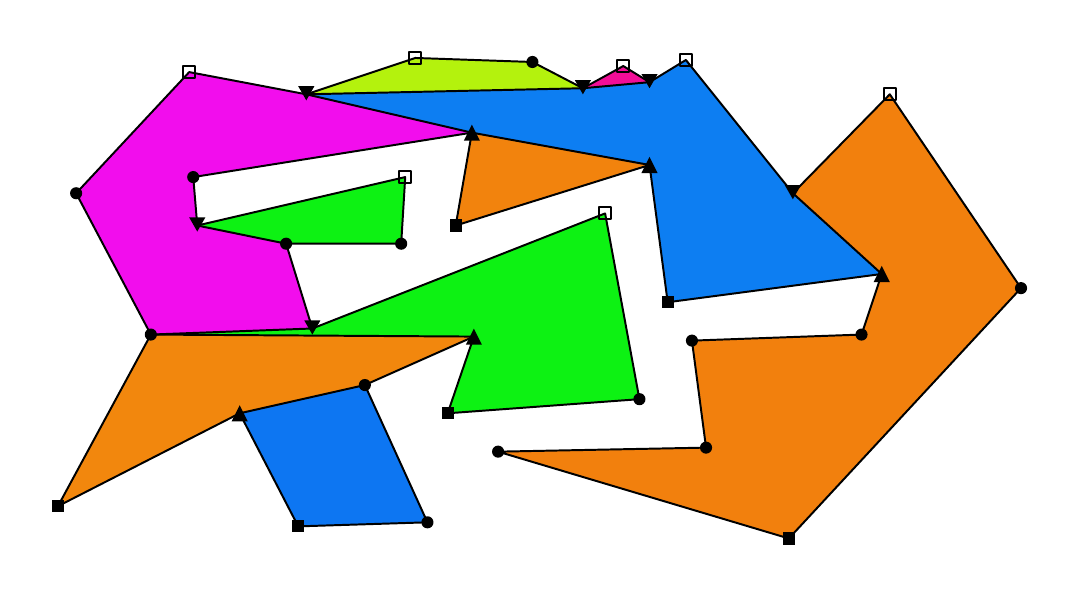
\begin{tikzpicture}[scale=13.0]
\clip (0,0) rectangle (1.000000,-0.528600);
\definecolor{FFFFFF}{rgb}{1.00000,1.00000,1.00000}
\definecolor{FF0000}{rgb}{1.00000,0.00000,0.00000}
\definecolor{F2800D}{rgb}{0.94902,0.50196,0.05098}
\definecolor{0D7EF2}{rgb}{0.05098,0.49412,0.94902}
\definecolor{F2830D}{rgb}{0.94902,0.51373,0.05098}
\definecolor{0DF213}{rgb}{0.05098,0.94902,0.07451}
\definecolor{0D76F2}{rgb}{0.05098,0.46275,0.94902}
\definecolor{F2870D}{rgb}{0.94902,0.52941,0.05098}
\definecolor{F20DED}{rgb}{0.94902,0.05098,0.92941}
\definecolor{B4F20D}{rgb}{0.70588,0.94902,0.05098}
\definecolor{F20D97}{rgb}{0.94902,0.05098,0.59216}
\definecolor{000000}{rgb}{0.00000,0.00000,0.00000}
\clip (0,0) rectangle (1,-1);
\fill[color=FFFFFF] (0.00000, 0.00000) rectangle (1.00000, -0.52860);
\fill[color=FF0000, opacity=0.40, even odd rule] (0.15779,-0.04339) -- (0.04734,-0.16174) -- (0.12032,-0.29980) -- (0.02959,-0.46746) -- (0.20710,-0.37673) -- (0.26430,-0.48718) -- (0.39053,-0.48323) -- (0.32939,-0.34911) -- (0.43590,-0.30178) -- (0.41026,-0.37673) -- (0.59763,-0.36292) -- (0.56410,-0.18146) -- (0.27811,-0.29389) -- (0.25247,-0.21105) -- (0.36489,-0.21105) -- (0.36884,-0.14596) -- (0.16568,-0.19329) -- (0.16174,-0.14596) -- (0.43393,-0.10256) -- (0.41815,-0.19329) -- (0.60750,-0.13412) -- (0.62525,-0.26824) -- (0.83432,-0.24063) -- (0.81460,-0.29980) -- (0.64892,-0.30572) -- (0.66272,-0.41026) -- (0.45957,-0.41420) -- (0.74359,-0.49901) -- (0.97041,-0.25444) -- (0.84221,-0.06509) -- (0.74753,-0.16174) -- (0.64300,-0.03156) -- (0.60750,-0.05325) -- (0.58185,-0.03748) -- (0.54241,-0.05917) -- (0.49310,-0.03353) -- (0.37870,-0.02959) -- (0.27219,-0.06509) -- cycle;
\fill[color=F2800D, even odd rule] (0.83432,-0.24063) -- (0.81460,-0.29980) -- (0.64892,-0.30572) -- (0.66272,-0.41026) -- (0.45957,-0.41420) -- (0.74359,-0.49901) -- (0.97041,-0.25444) -- (0.84221,-0.06509) -- (0.74753,-0.16174) -- cycle;
\fill[color=0D7EF2, even odd rule] (0.74753,-0.16174) -- (0.64300,-0.03156) -- (0.60750,-0.05325) -- (0.54241,-0.05917) -- (0.27219,-0.06509) -- (0.43393,-0.10256) -- (0.60750,-0.13412) -- (0.62525,-0.26824) -- (0.83432,-0.24063) -- cycle;
\fill[color=F2830D, even odd rule] (0.43393,-0.10256) -- (0.41815,-0.19329) -- (0.60750,-0.13412) -- cycle;
\fill[color=0DF213, even odd rule] (0.25247,-0.21105) -- (0.36489,-0.21105) -- (0.36884,-0.14596) -- (0.16568,-0.19329) -- cycle;
\fill[color=0DF213, even odd rule] (0.43590,-0.30178) -- (0.41026,-0.37673) -- (0.59763,-0.36292) -- (0.56410,-0.18146) -- (0.27811,-0.29389) -- (0.12032,-0.29980) -- cycle;
\fill[color=0D76F2, even odd rule] (0.20710,-0.37673) -- (0.26430,-0.48718) -- (0.39053,-0.48323) -- (0.32939,-0.34911) -- cycle;
\fill[color=F2870D, even odd rule] (0.32939,-0.34911) -- (0.43590,-0.30178) -- (0.12032,-0.29980) -- (0.02959,-0.46746) -- (0.20710,-0.37673) -- cycle;
\fill[color=F20DED, even odd rule] (0.27811,-0.29389) -- (0.25247,-0.21105) -- (0.16568,-0.19329) -- (0.16174,-0.14596) -- (0.43393,-0.10256) -- (0.27219,-0.06509) -- (0.15779,-0.04339) -- (0.04734,-0.16174) -- (0.12032,-0.29980) -- cycle;
\fill[color=B4F20D, even odd rule] (0.54241,-0.05917) -- (0.49310,-0.03353) -- (0.37870,-0.02959) -- (0.27219,-0.06509) -- cycle;
\fill[color=F20D97, even odd rule] (0.60750,-0.05325) -- (0.58185,-0.03748) -- (0.54241,-0.05917) -- cycle;
\draw[line width=0.25000mm, join=round, cap=round, color=000000] (0.54241,-0.05917) -- (0.60750,-0.05325);
\draw[line width=0.25000mm, join=round, cap=round, color=000000] (0.27219,-0.06509) -- (0.54241,-0.05917);
\draw[line width=0.25000mm, join=round, cap=round, color=000000] (0.43393,-0.10256) -- (0.27219,-0.06509);
\draw[line width=0.25000mm, join=round, cap=round, color=000000] (0.60750,-0.13412) -- (0.43393,-0.10256);
\draw[line width=0.25000mm, join=round, cap=round, color=000000] (0.25247,-0.21105) -- (0.16568,-0.19329);
\draw[line width=0.25000mm, join=round, cap=round, color=000000] (0.83432,-0.24063) -- (0.74753,-0.16174);
\draw[line width=0.25000mm, join=round, cap=round, color=000000] (0.12032,-0.29980) -- (0.27811,-0.29389);
\draw[line width=0.25000mm, join=round, cap=round, color=000000] (0.43590,-0.30178) -- (0.12032,-0.29980);
\draw[line width=0.25000mm, join=round, cap=round, color=000000] (0.20710,-0.37673) -- (0.32939,-0.34911);
\draw[line width=0.25000mm, join=round, cap=round, color=000000] (0.15779,-0.04339) -- (0.04734,-0.16174) -- (0.12032,-0.29980) -- (0.02959,-0.46746) -- (0.20710,-0.37673) -- (0.26430,-0.48718) -- (0.39053,-0.48323) -- (0.32939,-0.34911) -- (0.43590,-0.30178) -- (0.41026,-0.37673) -- (0.59763,-0.36292) -- (0.56410,-0.18146) -- (0.27811,-0.29389) -- (0.25247,-0.21105) -- (0.36489,-0.21105) -- (0.36884,-0.14596) -- (0.16568,-0.19329) -- (0.16174,-0.14596) -- (0.43393,-0.10256) -- (0.41815,-0.19329) -- (0.60750,-0.13412) -- (0.62525,-0.26824) -- (0.83432,-0.24063) -- (0.81460,-0.29980) -- (0.64892,-0.30572) -- (0.66272,-0.41026) -- (0.45957,-0.41420) -- (0.74359,-0.49901) -- (0.97041,-0.25444) -- (0.84221,-0.06509) -- (0.74753,-0.16174) -- (0.64300,-0.03156) -- (0.60750,-0.05325) -- (0.58185,-0.03748) -- (0.54241,-0.05917) -- (0.49310,-0.03353) -- (0.37870,-0.02959) -- (0.27219,-0.06509) -- cycle;
\draw[line width=0.25000mm, join=round, cap=round, color=000000]  (0.15187,-0.03748) -- (0.16371,-0.03748) -- (0.16371,-0.04931) -- (0.15187,-0.04931) -- (0.15187,-0.03748) -- cycle;
\fill[color=000000, even odd rule]  (0.04734,-0.16765) .. controls (0.04407,-0.16765) and (0.04142,-0.16500) .. (0.04142,-0.16174) .. controls (0.04142,-0.15847) and (0.04407,-0.15582) .. (0.04734,-0.15582) .. controls (0.05061,-0.15582) and (0.05325,-0.15847) .. (0.05325,-0.16174) .. controls (0.05325,-0.16500) and (0.05061,-0.16765) .. (0.04734,-0.16765) -- (0.04734,-0.16765) -- cycle;
\fill[color=000000, even odd rule]  (0.12032,-0.30572) .. controls (0.11705,-0.30572) and (0.11440,-0.30307) .. (0.11440,-0.29980) .. controls (0.11440,-0.29653) and (0.11705,-0.29389) .. (0.12032,-0.29389) .. controls (0.12358,-0.29389) and (0.12623,-0.29653) .. (0.12623,-0.29980) .. controls (0.12623,-0.30307) and (0.12358,-0.30572) .. (0.12032,-0.30572) -- (0.12032,-0.30572) -- cycle;
\fill[color=000000, even odd rule]  (0.02367,-0.47337) -- (0.02367,-0.46154) -- (0.03550,-0.46154) -- (0.03550,-0.47337) -- (0.02367,-0.47337) -- cycle;
\fill[color=000000, even odd rule]  (0.19921,-0.38462) -- (0.20710,-0.36884) -- (0.21499,-0.38462) -- (0.19921,-0.38462) -- cycle;
\fill[color=000000, even odd rule]  (0.25838,-0.49310) -- (0.25838,-0.48126) -- (0.27022,-0.48126) -- (0.27022,-0.49310) -- (0.25838,-0.49310) -- cycle;
\fill[color=000000, even odd rule]  (0.39053,-0.48915) .. controls (0.38726,-0.48915) and (0.38462,-0.48650) .. (0.38462,-0.48323) .. controls (0.38462,-0.47997) and (0.38726,-0.47732) .. (0.39053,-0.47732) .. controls (0.39380,-0.47732) and (0.39645,-0.47997) .. (0.39645,-0.48323) .. controls (0.39645,-0.48650) and (0.39380,-0.48915) .. (0.39053,-0.48915) -- (0.39053,-0.48915) -- cycle;
\fill[color=000000, even odd rule]  (0.32939,-0.35503) .. controls (0.32612,-0.35503) and (0.32347,-0.35238) .. (0.32347,-0.34911) .. controls (0.32347,-0.34584) and (0.32612,-0.34320) .. (0.32939,-0.34320) .. controls (0.33266,-0.34320) and (0.33531,-0.34584) .. (0.33531,-0.34911) .. controls (0.33531,-0.35238) and (0.33266,-0.35503) .. (0.32939,-0.35503) -- (0.32939,-0.35503) -- cycle;
\fill[color=000000, even odd rule]  (0.42801,-0.30966) -- (0.43590,-0.29389) -- (0.44379,-0.30966) -- (0.42801,-0.30966) -- cycle;
\fill[color=000000, even odd rule]  (0.40434,-0.38264) -- (0.40434,-0.37081) -- (0.41617,-0.37081) -- (0.41617,-0.38264) -- (0.40434,-0.38264) -- cycle;
\fill[color=000000, even odd rule]  (0.59763,-0.36884) .. controls (0.59437,-0.36884) and (0.59172,-0.36619) .. (0.59172,-0.36292) .. controls (0.59172,-0.35965) and (0.59437,-0.35700) .. (0.59763,-0.35700) .. controls (0.60090,-0.35700) and (0.60355,-0.35965) .. (0.60355,-0.36292) .. controls (0.60355,-0.36619) and (0.60090,-0.36884) .. (0.59763,-0.36884) -- (0.59763,-0.36884) -- cycle;
\draw[line width=0.25000mm, join=round, cap=round, color=000000]  (0.55819,-0.17554) -- (0.57002,-0.17554) -- (0.57002,-0.18738) -- (0.55819,-0.18738) -- (0.55819,-0.17554) -- cycle;
\fill[color=000000, even odd rule]  (0.27811,-0.29980) -- (0.27022,-0.28600) -- (0.28600,-0.28600) -- (0.27811,-0.29980) -- cycle;
\fill[color=000000, even odd rule]  (0.25247,-0.21696) .. controls (0.24920,-0.21696) and (0.24655,-0.21431) .. (0.24655,-0.21105) .. controls (0.24655,-0.20778) and (0.24920,-0.20513) .. (0.25247,-0.20513) .. controls (0.25573,-0.20513) and (0.25838,-0.20778) .. (0.25838,-0.21105) .. controls (0.25838,-0.21431) and (0.25573,-0.21696) .. (0.25247,-0.21696) -- (0.25247,-0.21696) -- cycle;
\fill[color=000000, even odd rule]  (0.36489,-0.21696) .. controls (0.36162,-0.21696) and (0.35897,-0.21431) .. (0.35897,-0.21105) .. controls (0.35897,-0.20778) and (0.36162,-0.20513) .. (0.36489,-0.20513) .. controls (0.36816,-0.20513) and (0.37081,-0.20778) .. (0.37081,-0.21105) .. controls (0.37081,-0.21431) and (0.36816,-0.21696) .. (0.36489,-0.21696) -- (0.36489,-0.21696) -- cycle;
\draw[line width=0.25000mm, join=round, cap=round, color=000000]  (0.36292,-0.14004) -- (0.37475,-0.14004) -- (0.37475,-0.15187) -- (0.36292,-0.15187) -- (0.36292,-0.14004) -- cycle;
\fill[color=000000, even odd rule]  (0.16568,-0.19921) -- (0.15779,-0.18540) -- (0.17357,-0.18540) -- (0.16568,-0.19921) -- cycle;
\fill[color=000000, even odd rule]  (0.16174,-0.15187) .. controls (0.15847,-0.15187) and (0.15582,-0.14922) .. (0.15582,-0.14596) .. controls (0.15582,-0.14269) and (0.15847,-0.14004) .. (0.16174,-0.14004) .. controls (0.16500,-0.14004) and (0.16765,-0.14269) .. (0.16765,-0.14596) .. controls (0.16765,-0.14922) and (0.16500,-0.15187) .. (0.16174,-0.15187) -- (0.16174,-0.15187) -- cycle;
\fill[color=000000, even odd rule]  (0.42604,-0.11045) -- (0.43393,-0.09467) -- (0.44181,-0.11045) -- (0.42604,-0.11045) -- cycle;
\fill[color=000000, even odd rule]  (0.41223,-0.19921) -- (0.41223,-0.18738) -- (0.42406,-0.18738) -- (0.42406,-0.19921) -- (0.41223,-0.19921) -- cycle;
\fill[color=000000, even odd rule]  (0.59961,-0.14201) -- (0.60750,-0.12623) -- (0.61538,-0.14201) -- (0.59961,-0.14201) -- cycle;
\fill[color=000000, even odd rule]  (0.61933,-0.27416) -- (0.61933,-0.26233) -- (0.63116,-0.26233) -- (0.63116,-0.27416) -- (0.61933,-0.27416) -- cycle;
\fill[color=000000, even odd rule]  (0.82643,-0.24852) -- (0.83432,-0.23274) -- (0.84221,-0.24852) -- (0.82643,-0.24852) -- cycle;
\fill[color=000000, even odd rule]  (0.81460,-0.30572) .. controls (0.81133,-0.30572) and (0.80868,-0.30307) .. (0.80868,-0.29980) .. controls (0.80868,-0.29653) and (0.81133,-0.29389) .. (0.81460,-0.29389) .. controls (0.81786,-0.29389) and (0.82051,-0.29653) .. (0.82051,-0.29980) .. controls (0.82051,-0.30307) and (0.81786,-0.30572) .. (0.81460,-0.30572) -- (0.81460,-0.30572) -- cycle;
\fill[color=000000, even odd rule]  (0.64892,-0.31164) .. controls (0.64565,-0.31164) and (0.64300,-0.30899) .. (0.64300,-0.30572) .. controls (0.64300,-0.30245) and (0.64565,-0.29980) .. (0.64892,-0.29980) .. controls (0.65218,-0.29980) and (0.65483,-0.30245) .. (0.65483,-0.30572) .. controls (0.65483,-0.30899) and (0.65218,-0.31164) .. (0.64892,-0.31164) -- (0.64892,-0.31164) -- cycle;
\fill[color=000000, even odd rule]  (0.66272,-0.41617) .. controls (0.65945,-0.41617) and (0.65680,-0.41352) .. (0.65680,-0.41026) .. controls (0.65680,-0.40699) and (0.65945,-0.40434) .. (0.66272,-0.40434) .. controls (0.66599,-0.40434) and (0.66864,-0.40699) .. (0.66864,-0.41026) .. controls (0.66864,-0.41352) and (0.66599,-0.41617) .. (0.66272,-0.41617) -- (0.66272,-0.41617) -- cycle;
\fill[color=000000, even odd rule]  (0.45957,-0.42012) .. controls (0.45630,-0.42012) and (0.45365,-0.41747) .. (0.45365,-0.41420) .. controls (0.45365,-0.41093) and (0.45630,-0.40828) .. (0.45957,-0.40828) .. controls (0.46283,-0.40828) and (0.46548,-0.41093) .. (0.46548,-0.41420) .. controls (0.46548,-0.41747) and (0.46283,-0.42012) .. (0.45957,-0.42012) -- (0.45957,-0.42012) -- cycle;
\fill[color=000000, even odd rule]  (0.73767,-0.50493) -- (0.73767,-0.49310) -- (0.74951,-0.49310) -- (0.74951,-0.50493) -- (0.73767,-0.50493) -- cycle;
\fill[color=000000, even odd rule]  (0.97041,-0.26036) .. controls (0.96715,-0.26036) and (0.96450,-0.25771) .. (0.96450,-0.25444) .. controls (0.96450,-0.25117) and (0.96715,-0.24852) .. (0.97041,-0.24852) .. controls (0.97368,-0.24852) and (0.97633,-0.25117) .. (0.97633,-0.25444) .. controls (0.97633,-0.25771) and (0.97368,-0.26036) .. (0.97041,-0.26036) -- (0.97041,-0.26036) -- cycle;
\draw[line width=0.25000mm, join=round, cap=round, color=000000]  (0.83629,-0.05917) -- (0.84813,-0.05917) -- (0.84813,-0.07101) -- (0.83629,-0.07101) -- (0.83629,-0.05917) -- cycle;
\fill[color=000000, even odd rule]  (0.74753,-0.16765) -- (0.73964,-0.15385) -- (0.75542,-0.15385) -- (0.74753,-0.16765) -- cycle;
\draw[line width=0.25000mm, join=round, cap=round, color=000000]  (0.63708,-0.02564) -- (0.64892,-0.02564) -- (0.64892,-0.03748) -- (0.63708,-0.03748) -- (0.63708,-0.02564) -- cycle;
\fill[color=000000, even odd rule]  (0.60750,-0.05917) -- (0.59961,-0.04536) -- (0.61538,-0.04536) -- (0.60750,-0.05917) -- cycle;
\draw[line width=0.25000mm, join=round, cap=round, color=000000]  (0.57594,-0.03156) -- (0.58777,-0.03156) -- (0.58777,-0.04339) -- (0.57594,-0.04339) -- (0.57594,-0.03156) -- cycle;
\fill[color=000000, even odd rule]  (0.54241,-0.06509) -- (0.53452,-0.05128) -- (0.55030,-0.05128) -- (0.54241,-0.06509) -- cycle;
\fill[color=000000, even odd rule]  (0.49310,-0.03945) .. controls (0.48983,-0.03945) and (0.48718,-0.03680) .. (0.48718,-0.03353) .. controls (0.48718,-0.03026) and (0.48983,-0.02761) .. (0.49310,-0.02761) .. controls (0.49636,-0.02761) and (0.49901,-0.03026) .. (0.49901,-0.03353) .. controls (0.49901,-0.03680) and (0.49636,-0.03945) .. (0.49310,-0.03945) -- (0.49310,-0.03945) -- cycle;
\draw[line width=0.25000mm, join=round, cap=round, color=000000]  (0.37278,-0.02367) -- (0.38462,-0.02367) -- (0.38462,-0.03550) -- (0.37278,-0.03550) -- (0.37278,-0.02367) -- cycle;
\fill[color=000000, even odd rule]  (0.27219,-0.07101) -- (0.26430,-0.05720) -- (0.28008,-0.05720) -- (0.27219,-0.07101) -- cycle;
\end{tikzpicture}
\end{center}
Also there should be some text below. This text block
should also be a not too short, so that there will be a line
break within the paragraph.
\begin{center}
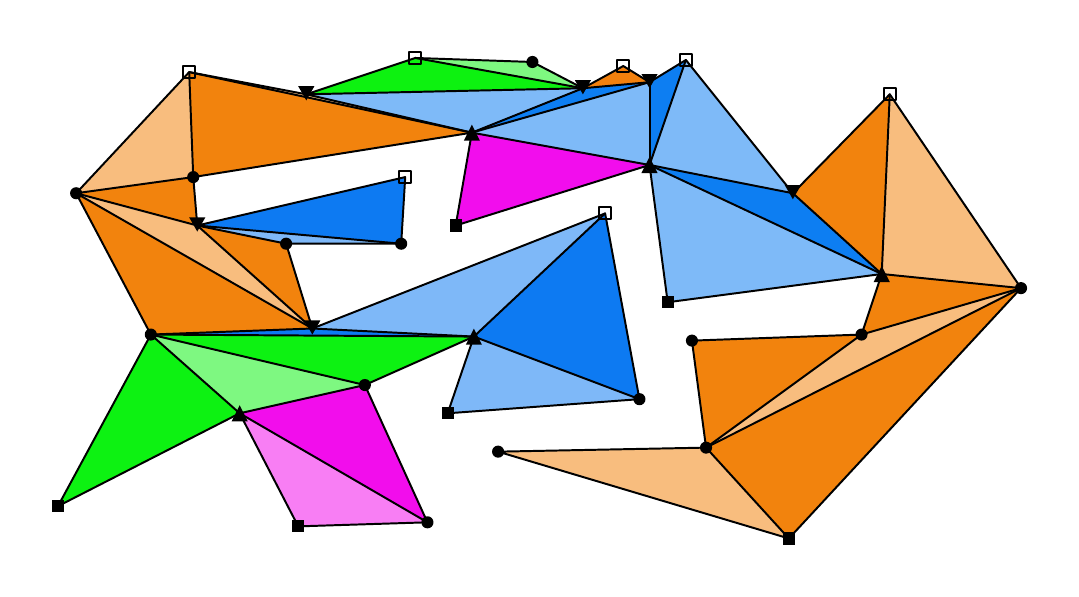
\begin{tikzpicture}[scale=13.0]
\clip (0,0) rectangle (1.000000,-0.528600);
\definecolor{FFFFFF}{rgb}{1.00000,1.00000,1.00000}
\definecolor{FF0000}{rgb}{1.00000,0.00000,0.00000}
\definecolor{F2830D}{rgb}{0.94902,0.51373,0.05098}
\definecolor{0D7EF2}{rgb}{0.05098,0.49412,0.94902}
\definecolor{F20DED}{rgb}{0.94902,0.05098,0.92941}
\definecolor{0D7AF2}{rgb}{0.05098,0.47843,0.94902}
\definecolor{F20DEC}{rgb}{0.94902,0.05098,0.92549}
\definecolor{0DF212}{rgb}{0.05098,0.94902,0.07059}
\definecolor{0DF210}{rgb}{0.05098,0.94902,0.06275}
\definecolor{F2800D}{rgb}{0.94902,0.50196,0.05098}
\definecolor{000000}{rgb}{0.00000,0.00000,0.00000}
\clip (0,0) rectangle (1,-1);
\fill[color=FFFFFF] (0.00000, 0.00000) rectangle (1.00000, -0.52860);
\fill[color=FF0000, opacity=0.40, even odd rule] (0.15779,-0.04339) -- (0.04734,-0.16174) -- (0.12032,-0.29980) -- (0.02959,-0.46746) -- (0.20710,-0.37673) -- (0.26430,-0.48718) -- (0.39053,-0.48323) -- (0.32939,-0.34911) -- (0.43590,-0.30178) -- (0.41026,-0.37673) -- (0.59763,-0.36292) -- (0.56410,-0.18146) -- (0.27811,-0.29389) -- (0.25247,-0.21105) -- (0.36489,-0.21105) -- (0.36884,-0.14596) -- (0.16568,-0.19329) -- (0.16174,-0.14596) -- (0.43393,-0.10256) -- (0.41815,-0.19329) -- (0.60750,-0.13412) -- (0.62525,-0.26824) -- (0.83432,-0.24063) -- (0.81460,-0.29980) -- (0.64892,-0.30572) -- (0.66272,-0.41026) -- (0.45957,-0.41420) -- (0.74359,-0.49901) -- (0.97041,-0.25444) -- (0.84221,-0.06509) -- (0.74753,-0.16174) -- (0.64300,-0.03156) -- (0.60750,-0.05325) -- (0.58185,-0.03748) -- (0.54241,-0.05917) -- (0.49310,-0.03353) -- (0.37870,-0.02959) -- (0.27219,-0.06509) -- cycle;
\fill[color=F2830D, even odd rule] (0.83432,-0.24063) -- (0.81460,-0.29980) -- (0.64892,-0.30572) -- (0.66272,-0.41026) -- (0.45957,-0.41420) -- (0.74359,-0.49901) -- (0.97041,-0.25444) -- (0.84221,-0.06509) -- (0.74753,-0.16174) -- cycle;
\fill[color=0D7EF2, even odd rule] (0.74753,-0.16174) -- (0.64300,-0.03156) -- (0.60750,-0.05325) -- (0.54241,-0.05917) -- (0.27219,-0.06509) -- (0.43393,-0.10256) -- (0.60750,-0.13412) -- (0.62525,-0.26824) -- (0.83432,-0.24063) -- cycle;
\fill[color=F20DED, even odd rule] (0.43393,-0.10256) -- (0.41815,-0.19329) -- (0.60750,-0.13412) -- cycle;
\fill[color=0D7AF2, even odd rule] (0.25247,-0.21105) -- (0.36489,-0.21105) -- (0.36884,-0.14596) -- (0.16568,-0.19329) -- cycle;
\fill[color=0D7AF2, even odd rule] (0.43590,-0.30178) -- (0.41026,-0.37673) -- (0.59763,-0.36292) -- (0.56410,-0.18146) -- (0.27811,-0.29389) -- (0.12032,-0.29980) -- cycle;
\fill[color=F20DEC, even odd rule] (0.20710,-0.37673) -- (0.26430,-0.48718) -- (0.39053,-0.48323) -- (0.32939,-0.34911) -- cycle;
\fill[color=0DF212, even odd rule] (0.32939,-0.34911) -- (0.43590,-0.30178) -- (0.12032,-0.29980) -- (0.02959,-0.46746) -- (0.20710,-0.37673) -- cycle;
\fill[color=F2830D, even odd rule] (0.27811,-0.29389) -- (0.25247,-0.21105) -- (0.16568,-0.19329) -- (0.16174,-0.14596) -- (0.43393,-0.10256) -- (0.27219,-0.06509) -- (0.15779,-0.04339) -- (0.04734,-0.16174) -- (0.12032,-0.29980) -- cycle;
\fill[color=0DF210, even odd rule] (0.54241,-0.05917) -- (0.49310,-0.03353) -- (0.37870,-0.02959) -- (0.27219,-0.06509) -- cycle;
\fill[color=F2800D, even odd rule] (0.60750,-0.05325) -- (0.58185,-0.03748) -- (0.54241,-0.05917) -- cycle;
\fill[color=FFFFFF, opacity=0.47, even odd rule] (0.97041,-0.25444) -- (0.84221,-0.06509) -- (0.83432,-0.24063) -- cycle;
\fill[color=FFFFFF, opacity=0.00, even odd rule] (0.74359,-0.49901) -- (0.97041,-0.25444) -- (0.66272,-0.41026) -- cycle;
\fill[color=FFFFFF, opacity=0.47, even odd rule] (0.66272,-0.41026) -- (0.45957,-0.41420) -- (0.74359,-0.49901) -- cycle;
\fill[color=FFFFFF, opacity=0.47, even odd rule] (0.97041,-0.25444) -- (0.81460,-0.29980) -- (0.66272,-0.41026) -- cycle;
\fill[color=FFFFFF, opacity=0.00, even odd rule] (0.81460,-0.29980) -- (0.64892,-0.30572) -- (0.66272,-0.41026) -- cycle;
\fill[color=FFFFFF, opacity=0.00, even odd rule] (0.97041,-0.25444) -- (0.83432,-0.24063) -- (0.81460,-0.29980) -- cycle;
\fill[color=FFFFFF, opacity=0.00, even odd rule] (0.84221,-0.06509) -- (0.74753,-0.16174) -- (0.83432,-0.24063) -- cycle;
\fill[color=FFFFFF, opacity=0.47, even odd rule] (0.74753,-0.16174) -- (0.64300,-0.03156) -- (0.60750,-0.13412) -- cycle;
\fill[color=FFFFFF, opacity=0.00, even odd rule] (0.83432,-0.24063) -- (0.74753,-0.16174) -- (0.60750,-0.13412) -- cycle;
\fill[color=FFFFFF, opacity=0.47, even odd rule] (0.60750,-0.13412) -- (0.62525,-0.26824) -- (0.83432,-0.24063) -- cycle;
\fill[color=FFFFFF, opacity=0.00, even odd rule] (0.64300,-0.03156) -- (0.60750,-0.05325) -- (0.60750,-0.13412) -- cycle;
\fill[color=FFFFFF, opacity=0.47, even odd rule] (0.60750,-0.05325) -- (0.43393,-0.10256) -- (0.60750,-0.13412) -- cycle;
\fill[color=FFFFFF, opacity=0.00, even odd rule] (0.60750,-0.05325) -- (0.54241,-0.05917) -- (0.43393,-0.10256) -- cycle;
\fill[color=FFFFFF, opacity=0.47, even odd rule] (0.54241,-0.05917) -- (0.27219,-0.06509) -- (0.43393,-0.10256) -- cycle;
\fill[color=FFFFFF, opacity=0.00, even odd rule] (0.43393,-0.10256) -- (0.41815,-0.19329) -- (0.60750,-0.13412) -- cycle;
\fill[color=FFFFFF, opacity=0.00, even odd rule] (0.36489,-0.21105) -- (0.36884,-0.14596) -- (0.16568,-0.19329) -- cycle;
\fill[color=FFFFFF, opacity=0.47, even odd rule] (0.16568,-0.19329) -- (0.25247,-0.21105) -- (0.36489,-0.21105) -- cycle;
\fill[color=FFFFFF, opacity=0.00, even odd rule] (0.59763,-0.36292) -- (0.56410,-0.18146) -- (0.43590,-0.30178) -- cycle;
\fill[color=FFFFFF, opacity=0.47, even odd rule] (0.43590,-0.30178) -- (0.41026,-0.37673) -- (0.59763,-0.36292) -- cycle;
\fill[color=FFFFFF, opacity=0.47, even odd rule] (0.56410,-0.18146) -- (0.27811,-0.29389) -- (0.43590,-0.30178) -- cycle;
\fill[color=FFFFFF, opacity=0.00, even odd rule] (0.27811,-0.29389) -- (0.12032,-0.29980) -- (0.43590,-0.30178) -- cycle;
\fill[color=FFFFFF, opacity=0.00, even odd rule] (0.39053,-0.48323) -- (0.32939,-0.34911) -- (0.20710,-0.37673) -- cycle;
\fill[color=FFFFFF, opacity=0.47, even odd rule] (0.20710,-0.37673) -- (0.26430,-0.48718) -- (0.39053,-0.48323) -- cycle;
\fill[color=FFFFFF, opacity=0.00, even odd rule] (0.32939,-0.34911) -- (0.43590,-0.30178) -- (0.12032,-0.29980) -- cycle;
\fill[color=FFFFFF, opacity=0.47, even odd rule] (0.20710,-0.37673) -- (0.32939,-0.34911) -- (0.12032,-0.29980) -- cycle;
\fill[color=FFFFFF, opacity=0.00, even odd rule] (0.12032,-0.29980) -- (0.02959,-0.46746) -- (0.20710,-0.37673) -- cycle;
\fill[color=FFFFFF, opacity=0.47, even odd rule] (0.43393,-0.10256) -- (0.27219,-0.06509) -- (0.15779,-0.04339) -- cycle;
\fill[color=FFFFFF, opacity=0.00, even odd rule] (0.16174,-0.14596) -- (0.43393,-0.10256) -- (0.15779,-0.04339) -- cycle;
\fill[color=FFFFFF, opacity=0.00, even odd rule] (0.16568,-0.19329) -- (0.16174,-0.14596) -- (0.04734,-0.16174) -- cycle;
\fill[color=FFFFFF, opacity=0.00, even odd rule] (0.27811,-0.29389) -- (0.25247,-0.21105) -- (0.16568,-0.19329) -- cycle;
\fill[color=FFFFFF, opacity=0.47, even odd rule] (0.27811,-0.29389) -- (0.16568,-0.19329) -- (0.04734,-0.16174) -- cycle;
\fill[color=FFFFFF, opacity=0.00, even odd rule] (0.04734,-0.16174) -- (0.12032,-0.29980) -- (0.27811,-0.29389) -- cycle;
\fill[color=FFFFFF, opacity=0.47, even odd rule] (0.16174,-0.14596) -- (0.15779,-0.04339) -- (0.04734,-0.16174) -- cycle;
\fill[color=FFFFFF, opacity=0.47, even odd rule] (0.54241,-0.05917) -- (0.49310,-0.03353) -- (0.37870,-0.02959) -- cycle;
\fill[color=FFFFFF, opacity=0.00, even odd rule] (0.37870,-0.02959) -- (0.27219,-0.06509) -- (0.54241,-0.05917) -- cycle;
\fill[color=FFFFFF, opacity=0.00, even odd rule] (0.60750,-0.05325) -- (0.58185,-0.03748) -- (0.54241,-0.05917) -- cycle;
\draw[line width=0.25000mm, join=round, cap=round, color=000000] (0.83432,-0.24063) -- (0.84221,-0.06509);
\draw[line width=0.25000mm, join=round, cap=round, color=000000] (0.97041,-0.25444) -- (0.83432,-0.24063);
\draw[line width=0.25000mm, join=round, cap=round, color=000000] (0.81460,-0.29980) -- (0.97041,-0.25444);
\draw[line width=0.25000mm, join=round, cap=round, color=000000] (0.66272,-0.41026) -- (0.81460,-0.29980);
\draw[line width=0.25000mm, join=round, cap=round, color=000000] (0.66272,-0.41026) -- (0.97041,-0.25444);
\draw[line width=0.25000mm, join=round, cap=round, color=000000] (0.74359,-0.49901) -- (0.66272,-0.41026);
\draw[line width=0.25000mm, join=round, cap=round, color=000000] (0.43393,-0.10256) -- (0.54241,-0.05917);
\draw[line width=0.25000mm, join=round, cap=round, color=000000] (0.43393,-0.10256) -- (0.60750,-0.05325);
\draw[line width=0.25000mm, join=round, cap=round, color=000000] (0.60750,-0.13412) -- (0.60750,-0.05325);
\draw[line width=0.25000mm, join=round, cap=round, color=000000] (0.60750,-0.13412) -- (0.64300,-0.03156);
\draw[line width=0.25000mm, join=round, cap=round, color=000000] (0.74753,-0.16174) -- (0.60750,-0.13412);
\draw[line width=0.25000mm, join=round, cap=round, color=000000] (0.83432,-0.24063) -- (0.60750,-0.13412);
\draw[line width=0.25000mm, join=round, cap=round, color=000000] (0.36489,-0.21105) -- (0.16568,-0.19329);
\draw[line width=0.25000mm, join=round, cap=round, color=000000] (0.43590,-0.30178) -- (0.27811,-0.29389);
\draw[line width=0.25000mm, join=round, cap=round, color=000000] (0.43590,-0.30178) -- (0.56410,-0.18146);
\draw[line width=0.25000mm, join=round, cap=round, color=000000] (0.59763,-0.36292) -- (0.43590,-0.30178);
\draw[line width=0.25000mm, join=round, cap=round, color=000000] (0.39053,-0.48323) -- (0.20710,-0.37673);
\draw[line width=0.25000mm, join=round, cap=round, color=000000] (0.32939,-0.34911) -- (0.12032,-0.29980);
\draw[line width=0.25000mm, join=round, cap=round, color=000000] (0.20710,-0.37673) -- (0.12032,-0.29980);
\draw[line width=0.25000mm, join=round, cap=round, color=000000] (0.43393,-0.10256) -- (0.15779,-0.04339);
\draw[line width=0.25000mm, join=round, cap=round, color=000000] (0.16174,-0.14596) -- (0.15779,-0.04339);
\draw[line width=0.25000mm, join=round, cap=round, color=000000] (0.04734,-0.16174) -- (0.16174,-0.14596);
\draw[line width=0.25000mm, join=round, cap=round, color=000000] (0.16568,-0.19329) -- (0.04734,-0.16174);
\draw[line width=0.25000mm, join=round, cap=round, color=000000] (0.27811,-0.29389) -- (0.16568,-0.19329);
\draw[line width=0.25000mm, join=round, cap=round, color=000000] (0.27811,-0.29389) -- (0.04734,-0.16174);
\draw[line width=0.25000mm, join=round, cap=round, color=000000] (0.54241,-0.05917) -- (0.37870,-0.02959);
\draw[line width=0.25000mm, join=round, cap=round, color=000000] (0.54241,-0.05917) -- (0.60750,-0.05325);
\draw[line width=0.25000mm, join=round, cap=round, color=000000] (0.27219,-0.06509) -- (0.54241,-0.05917);
\draw[line width=0.25000mm, join=round, cap=round, color=000000] (0.43393,-0.10256) -- (0.27219,-0.06509);
\draw[line width=0.25000mm, join=round, cap=round, color=000000] (0.60750,-0.13412) -- (0.43393,-0.10256);
\draw[line width=0.25000mm, join=round, cap=round, color=000000] (0.25247,-0.21105) -- (0.16568,-0.19329);
\draw[line width=0.25000mm, join=round, cap=round, color=000000] (0.83432,-0.24063) -- (0.74753,-0.16174);
\draw[line width=0.25000mm, join=round, cap=round, color=000000] (0.12032,-0.29980) -- (0.27811,-0.29389);
\draw[line width=0.25000mm, join=round, cap=round, color=000000] (0.43590,-0.30178) -- (0.12032,-0.29980);
\draw[line width=0.25000mm, join=round, cap=round, color=000000] (0.20710,-0.37673) -- (0.32939,-0.34911);
\draw[line width=0.25000mm, join=round, cap=round, color=000000] (0.15779,-0.04339) -- (0.04734,-0.16174) -- (0.12032,-0.29980) -- (0.02959,-0.46746) -- (0.20710,-0.37673) -- (0.26430,-0.48718) -- (0.39053,-0.48323) -- (0.32939,-0.34911) -- (0.43590,-0.30178) -- (0.41026,-0.37673) -- (0.59763,-0.36292) -- (0.56410,-0.18146) -- (0.27811,-0.29389) -- (0.25247,-0.21105) -- (0.36489,-0.21105) -- (0.36884,-0.14596) -- (0.16568,-0.19329) -- (0.16174,-0.14596) -- (0.43393,-0.10256) -- (0.41815,-0.19329) -- (0.60750,-0.13412) -- (0.62525,-0.26824) -- (0.83432,-0.24063) -- (0.81460,-0.29980) -- (0.64892,-0.30572) -- (0.66272,-0.41026) -- (0.45957,-0.41420) -- (0.74359,-0.49901) -- (0.97041,-0.25444) -- (0.84221,-0.06509) -- (0.74753,-0.16174) -- (0.64300,-0.03156) -- (0.60750,-0.05325) -- (0.58185,-0.03748) -- (0.54241,-0.05917) -- (0.49310,-0.03353) -- (0.37870,-0.02959) -- (0.27219,-0.06509) -- cycle;
\draw[line width=0.25000mm, join=round, cap=round, color=000000]  (0.15187,-0.03748) -- (0.16371,-0.03748) -- (0.16371,-0.04931) -- (0.15187,-0.04931) -- (0.15187,-0.03748) -- cycle;
\fill[color=000000, even odd rule]  (0.04734,-0.16765) .. controls (0.04407,-0.16765) and (0.04142,-0.16500) .. (0.04142,-0.16174) .. controls (0.04142,-0.15847) and (0.04407,-0.15582) .. (0.04734,-0.15582) .. controls (0.05061,-0.15582) and (0.05325,-0.15847) .. (0.05325,-0.16174) .. controls (0.05325,-0.16500) and (0.05061,-0.16765) .. (0.04734,-0.16765) -- (0.04734,-0.16765) -- cycle;
\fill[color=000000, even odd rule]  (0.12032,-0.30572) .. controls (0.11705,-0.30572) and (0.11440,-0.30307) .. (0.11440,-0.29980) .. controls (0.11440,-0.29653) and (0.11705,-0.29389) .. (0.12032,-0.29389) .. controls (0.12358,-0.29389) and (0.12623,-0.29653) .. (0.12623,-0.29980) .. controls (0.12623,-0.30307) and (0.12358,-0.30572) .. (0.12032,-0.30572) -- (0.12032,-0.30572) -- cycle;
\fill[color=000000, even odd rule]  (0.02367,-0.47337) -- (0.02367,-0.46154) -- (0.03550,-0.46154) -- (0.03550,-0.47337) -- (0.02367,-0.47337) -- cycle;
\fill[color=000000, even odd rule]  (0.19921,-0.38462) -- (0.20710,-0.36884) -- (0.21499,-0.38462) -- (0.19921,-0.38462) -- cycle;
\fill[color=000000, even odd rule]  (0.25838,-0.49310) -- (0.25838,-0.48126) -- (0.27022,-0.48126) -- (0.27022,-0.49310) -- (0.25838,-0.49310) -- cycle;
\fill[color=000000, even odd rule]  (0.39053,-0.48915) .. controls (0.38726,-0.48915) and (0.38462,-0.48650) .. (0.38462,-0.48323) .. controls (0.38462,-0.47997) and (0.38726,-0.47732) .. (0.39053,-0.47732) .. controls (0.39380,-0.47732) and (0.39645,-0.47997) .. (0.39645,-0.48323) .. controls (0.39645,-0.48650) and (0.39380,-0.48915) .. (0.39053,-0.48915) -- (0.39053,-0.48915) -- cycle;
\fill[color=000000, even odd rule]  (0.32939,-0.35503) .. controls (0.32612,-0.35503) and (0.32347,-0.35238) .. (0.32347,-0.34911) .. controls (0.32347,-0.34584) and (0.32612,-0.34320) .. (0.32939,-0.34320) .. controls (0.33266,-0.34320) and (0.33531,-0.34584) .. (0.33531,-0.34911) .. controls (0.33531,-0.35238) and (0.33266,-0.35503) .. (0.32939,-0.35503) -- (0.32939,-0.35503) -- cycle;
\fill[color=000000, even odd rule]  (0.42801,-0.30966) -- (0.43590,-0.29389) -- (0.44379,-0.30966) -- (0.42801,-0.30966) -- cycle;
\fill[color=000000, even odd rule]  (0.40434,-0.38264) -- (0.40434,-0.37081) -- (0.41617,-0.37081) -- (0.41617,-0.38264) -- (0.40434,-0.38264) -- cycle;
\fill[color=000000, even odd rule]  (0.59763,-0.36884) .. controls (0.59437,-0.36884) and (0.59172,-0.36619) .. (0.59172,-0.36292) .. controls (0.59172,-0.35965) and (0.59437,-0.35700) .. (0.59763,-0.35700) .. controls (0.60090,-0.35700) and (0.60355,-0.35965) .. (0.60355,-0.36292) .. controls (0.60355,-0.36619) and (0.60090,-0.36884) .. (0.59763,-0.36884) -- (0.59763,-0.36884) -- cycle;
\draw[line width=0.25000mm, join=round, cap=round, color=000000]  (0.55819,-0.17554) -- (0.57002,-0.17554) -- (0.57002,-0.18738) -- (0.55819,-0.18738) -- (0.55819,-0.17554) -- cycle;
\fill[color=000000, even odd rule]  (0.27811,-0.29980) -- (0.27022,-0.28600) -- (0.28600,-0.28600) -- (0.27811,-0.29980) -- cycle;
\fill[color=000000, even odd rule]  (0.25247,-0.21696) .. controls (0.24920,-0.21696) and (0.24655,-0.21431) .. (0.24655,-0.21105) .. controls (0.24655,-0.20778) and (0.24920,-0.20513) .. (0.25247,-0.20513) .. controls (0.25573,-0.20513) and (0.25838,-0.20778) .. (0.25838,-0.21105) .. controls (0.25838,-0.21431) and (0.25573,-0.21696) .. (0.25247,-0.21696) -- (0.25247,-0.21696) -- cycle;
\fill[color=000000, even odd rule]  (0.36489,-0.21696) .. controls (0.36162,-0.21696) and (0.35897,-0.21431) .. (0.35897,-0.21105) .. controls (0.35897,-0.20778) and (0.36162,-0.20513) .. (0.36489,-0.20513) .. controls (0.36816,-0.20513) and (0.37081,-0.20778) .. (0.37081,-0.21105) .. controls (0.37081,-0.21431) and (0.36816,-0.21696) .. (0.36489,-0.21696) -- (0.36489,-0.21696) -- cycle;
\draw[line width=0.25000mm, join=round, cap=round, color=000000]  (0.36292,-0.14004) -- (0.37475,-0.14004) -- (0.37475,-0.15187) -- (0.36292,-0.15187) -- (0.36292,-0.14004) -- cycle;
\fill[color=000000, even odd rule]  (0.16568,-0.19921) -- (0.15779,-0.18540) -- (0.17357,-0.18540) -- (0.16568,-0.19921) -- cycle;
\fill[color=000000, even odd rule]  (0.16174,-0.15187) .. controls (0.15847,-0.15187) and (0.15582,-0.14922) .. (0.15582,-0.14596) .. controls (0.15582,-0.14269) and (0.15847,-0.14004) .. (0.16174,-0.14004) .. controls (0.16500,-0.14004) and (0.16765,-0.14269) .. (0.16765,-0.14596) .. controls (0.16765,-0.14922) and (0.16500,-0.15187) .. (0.16174,-0.15187) -- (0.16174,-0.15187) -- cycle;
\fill[color=000000, even odd rule]  (0.42604,-0.11045) -- (0.43393,-0.09467) -- (0.44181,-0.11045) -- (0.42604,-0.11045) -- cycle;
\fill[color=000000, even odd rule]  (0.41223,-0.19921) -- (0.41223,-0.18738) -- (0.42406,-0.18738) -- (0.42406,-0.19921) -- (0.41223,-0.19921) -- cycle;
\fill[color=000000, even odd rule]  (0.59961,-0.14201) -- (0.60750,-0.12623) -- (0.61538,-0.14201) -- (0.59961,-0.14201) -- cycle;
\fill[color=000000, even odd rule]  (0.61933,-0.27416) -- (0.61933,-0.26233) -- (0.63116,-0.26233) -- (0.63116,-0.27416) -- (0.61933,-0.27416) -- cycle;
\fill[color=000000, even odd rule]  (0.82643,-0.24852) -- (0.83432,-0.23274) -- (0.84221,-0.24852) -- (0.82643,-0.24852) -- cycle;
\fill[color=000000, even odd rule]  (0.81460,-0.30572) .. controls (0.81133,-0.30572) and (0.80868,-0.30307) .. (0.80868,-0.29980) .. controls (0.80868,-0.29653) and (0.81133,-0.29389) .. (0.81460,-0.29389) .. controls (0.81786,-0.29389) and (0.82051,-0.29653) .. (0.82051,-0.29980) .. controls (0.82051,-0.30307) and (0.81786,-0.30572) .. (0.81460,-0.30572) -- (0.81460,-0.30572) -- cycle;
\fill[color=000000, even odd rule]  (0.64892,-0.31164) .. controls (0.64565,-0.31164) and (0.64300,-0.30899) .. (0.64300,-0.30572) .. controls (0.64300,-0.30245) and (0.64565,-0.29980) .. (0.64892,-0.29980) .. controls (0.65218,-0.29980) and (0.65483,-0.30245) .. (0.65483,-0.30572) .. controls (0.65483,-0.30899) and (0.65218,-0.31164) .. (0.64892,-0.31164) -- (0.64892,-0.31164) -- cycle;
\fill[color=000000, even odd rule]  (0.66272,-0.41617) .. controls (0.65945,-0.41617) and (0.65680,-0.41352) .. (0.65680,-0.41026) .. controls (0.65680,-0.40699) and (0.65945,-0.40434) .. (0.66272,-0.40434) .. controls (0.66599,-0.40434) and (0.66864,-0.40699) .. (0.66864,-0.41026) .. controls (0.66864,-0.41352) and (0.66599,-0.41617) .. (0.66272,-0.41617) -- (0.66272,-0.41617) -- cycle;
\fill[color=000000, even odd rule]  (0.45957,-0.42012) .. controls (0.45630,-0.42012) and (0.45365,-0.41747) .. (0.45365,-0.41420) .. controls (0.45365,-0.41093) and (0.45630,-0.40828) .. (0.45957,-0.40828) .. controls (0.46283,-0.40828) and (0.46548,-0.41093) .. (0.46548,-0.41420) .. controls (0.46548,-0.41747) and (0.46283,-0.42012) .. (0.45957,-0.42012) -- (0.45957,-0.42012) -- cycle;
\fill[color=000000, even odd rule]  (0.73767,-0.50493) -- (0.73767,-0.49310) -- (0.74951,-0.49310) -- (0.74951,-0.50493) -- (0.73767,-0.50493) -- cycle;
\fill[color=000000, even odd rule]  (0.97041,-0.26036) .. controls (0.96715,-0.26036) and (0.96450,-0.25771) .. (0.96450,-0.25444) .. controls (0.96450,-0.25117) and (0.96715,-0.24852) .. (0.97041,-0.24852) .. controls (0.97368,-0.24852) and (0.97633,-0.25117) .. (0.97633,-0.25444) .. controls (0.97633,-0.25771) and (0.97368,-0.26036) .. (0.97041,-0.26036) -- (0.97041,-0.26036) -- cycle;
\draw[line width=0.25000mm, join=round, cap=round, color=000000]  (0.83629,-0.05917) -- (0.84813,-0.05917) -- (0.84813,-0.07101) -- (0.83629,-0.07101) -- (0.83629,-0.05917) -- cycle;
\fill[color=000000, even odd rule]  (0.74753,-0.16765) -- (0.73964,-0.15385) -- (0.75542,-0.15385) -- (0.74753,-0.16765) -- cycle;
\draw[line width=0.25000mm, join=round, cap=round, color=000000]  (0.63708,-0.02564) -- (0.64892,-0.02564) -- (0.64892,-0.03748) -- (0.63708,-0.03748) -- (0.63708,-0.02564) -- cycle;
\fill[color=000000, even odd rule]  (0.60750,-0.05917) -- (0.59961,-0.04536) -- (0.61538,-0.04536) -- (0.60750,-0.05917) -- cycle;
\draw[line width=0.25000mm, join=round, cap=round, color=000000]  (0.57594,-0.03156) -- (0.58777,-0.03156) -- (0.58777,-0.04339) -- (0.57594,-0.04339) -- (0.57594,-0.03156) -- cycle;
\fill[color=000000, even odd rule]  (0.54241,-0.06509) -- (0.53452,-0.05128) -- (0.55030,-0.05128) -- (0.54241,-0.06509) -- cycle;
\fill[color=000000, even odd rule]  (0.49310,-0.03945) .. controls (0.48983,-0.03945) and (0.48718,-0.03680) .. (0.48718,-0.03353) .. controls (0.48718,-0.03026) and (0.48983,-0.02761) .. (0.49310,-0.02761) .. controls (0.49636,-0.02761) and (0.49901,-0.03026) .. (0.49901,-0.03353) .. controls (0.49901,-0.03680) and (0.49636,-0.03945) .. (0.49310,-0.03945) -- (0.49310,-0.03945) -- cycle;
\draw[line width=0.25000mm, join=round, cap=round, color=000000]  (0.37278,-0.02367) -- (0.38462,-0.02367) -- (0.38462,-0.03550) -- (0.37278,-0.03550) -- (0.37278,-0.02367) -- cycle;
\fill[color=000000, even odd rule]  (0.27219,-0.07101) -- (0.26430,-0.05720) -- (0.28008,-0.05720) -- (0.27219,-0.07101) -- cycle;
\end{tikzpicture}
\end{center}
Also there should be some text below. This text block
should also be a not too short, so that there will be a line
break within the paragraph.
\begin{center}
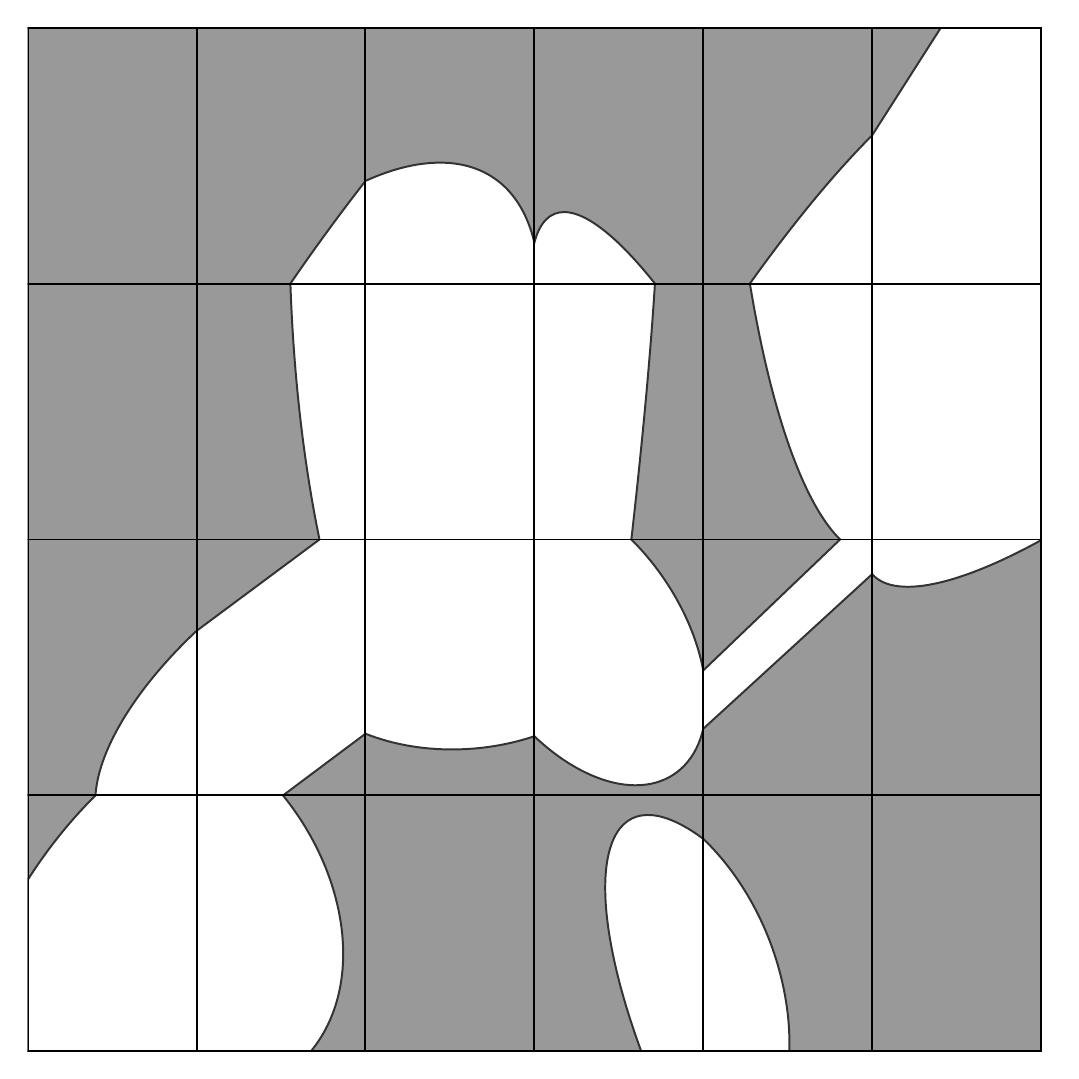
\begin{tikzpicture}[scale=13.0]
\clip (0,0) rectangle (1.000000,-1.000000);
\definecolor{999999}{rgb}{0.60000,0.60000,0.60000}
\definecolor{FFFFFF}{rgb}{1.00000,1.00000,1.00000}
\definecolor{333333}{rgb}{0.20000,0.20000,0.20000}
\definecolor{000000}{rgb}{0.00000,0.00000,0.00000}
\clip (0,0) rectangle (1,-1);
\fill[color=999999] (0.00000, 0.00000) rectangle (0.16500, -0.25000);
\begin{scope}
\clip  (0.00000,-0.00000) -- (0.16500,0.00000) -- (0.16500,-0.25000) -- (0.00000,-0.25000) -- (0.00000,0.00000) -- cycle;
\fill[color=FFFFFF, even odd rule]  (0.00000,-1.00000) -- (0.00000,-0.57707) .. controls (0.02099,-0.55167) and (0.04163,-0.52750) .. (0.06177,-0.50477) .. controls (0.16830,-0.38458) and (0.24256,-0.32559) .. (0.27883,-0.32559) .. controls (0.32204,-0.32559) and (0.31135,-0.40928) .. (0.23711,-0.57289) .. controls (0.18086,-0.69687) and (0.09688,-0.84741) .. (0.00125,-1.00000) -- (0.00000,-1.00000) -- cycle;
\end{scope}
\begin{scope}
\clip  (0.00000,-0.00000) -- (0.16500,0.00000) -- (0.16500,-0.25000) -- (0.00000,-0.25000) -- (0.00000,0.00000) -- cycle;
\draw[line width=0.25000mm, join=round, cap=round, color=333333]  (0.00000,-1.00000) -- (0.00000,-1.00000) -- (0.00125,-1.00000) .. controls (0.09688,-0.84741) and (0.18086,-0.69687) .. (0.23711,-0.57289) .. controls (0.37368,-0.27192) and (0.29518,-0.24142) .. (0.06177,-0.50477) .. controls (0.04163,-0.52750) and (0.02099,-0.55167) .. (0.00000,-0.57707) -- (0.00000,-1.00000) -- cycle;
\end{scope}
\fill[color=999999] (0.00000, -0.25000) rectangle (0.16500, -0.50000);
\begin{scope}
\clip  (0.00000,-0.25000) -- (0.16500,-0.25000) -- (0.16500,-0.50000) -- (0.00000,-0.50000) -- (0.00000,-0.25000) -- cycle;
\fill[color=FFFFFF, even odd rule]  (0.34133,-1.00000) -- (0.34133,-1.00000) .. controls (0.31321,-0.83604) and (0.29573,-0.68290) .. (0.29347,-0.56271) .. controls (0.29069,-0.41518) and (0.31130,-0.34279) .. (0.34758,-0.34279) .. controls (0.39078,-0.34279) and (0.45620,-0.44550) .. (0.53076,-0.64632) .. controls (0.56995,-0.75188) and (0.60742,-0.87312) .. (0.64110,-1.00000) -- (0.34133,-1.00000) -- cycle;
\end{scope}
\begin{scope}
\clip  (0.00000,-0.25000) -- (0.16500,-0.25000) -- (0.16500,-0.50000) -- (0.00000,-0.50000) -- (0.00000,-0.25000) -- cycle;
\draw[line width=0.25000mm, join=round, cap=round, color=333333]  (0.79012,-1.00000) -- (0.64110,-1.00000) .. controls (0.60742,-0.87312) and (0.56995,-0.75188) .. (0.53076,-0.64632) .. controls (0.39361,-0.27690) and (0.28737,-0.23947) .. (0.29347,-0.56271) .. controls (0.29573,-0.68290) and (0.31321,-0.83604) .. (0.34133,-1.00000) -- (0.55283,-1.00000) -- (0.79012,-1.00000) -- cycle;
\end{scope}
\fill[color=999999] (0.00000, -0.50000) rectangle (0.16500, -0.75000);
\begin{scope}
\clip  (0.00000,-0.50000) -- (0.16500,-0.50000) -- (0.16500,-0.75000) -- (0.00000,-0.75000) -- (0.00000,-0.50000) -- cycle;
\fill[color=FFFFFF, even odd rule]  (0.13704,-0.81564) .. controls (0.09383,-0.81564) and (0.06638,-0.79563) .. (0.06605,-0.75651) .. controls (0.06546,-0.68456) and (0.15690,-0.57518) .. (0.27029,-0.51221) .. controls (0.32204,-0.48348) and (0.36942,-0.46938) .. (0.40569,-0.46938) .. controls (0.44890,-0.46938) and (0.47635,-0.48938) .. (0.47667,-0.52850) .. controls (0.47727,-0.60046) and (0.38583,-0.70984) .. (0.27244,-0.77280) -- (0.27244,-0.77280) .. controls (0.22069,-0.80154) and (0.17331,-0.81564) .. (0.13704,-0.81564) -- (0.13704,-0.81564) -- cycle;
\end{scope}
\begin{scope}
\clip  (0.00000,-0.50000) -- (0.16500,-0.50000) -- (0.16500,-0.75000) -- (0.00000,-0.75000) -- (0.00000,-0.50000) -- cycle;
\draw[line width=0.25000mm, join=round, cap=round, color=333333]  (0.27244,-0.77280) .. controls (0.38583,-0.70984) and (0.47727,-0.60046) .. (0.47667,-0.52850) .. controls (0.47608,-0.45654) and (0.38368,-0.44925) .. (0.27029,-0.51221) .. controls (0.15690,-0.57518) and (0.06546,-0.68456) .. (0.06605,-0.75651) .. controls (0.06665,-0.82847) and (0.15905,-0.83577) .. (0.27244,-0.77280) -- (0.27244,-0.77280) -- cycle;
\end{scope}
\fill[color=999999] (0.00000, -0.75000) rectangle (0.16500, -1.00000);
\begin{scope}
\clip  (0.00000,-0.75000) -- (0.16500,-0.75000) -- (0.16500,-1.00000) -- (0.00000,-1.00000) -- (0.00000,-0.75000) -- cycle;
\fill[color=FFFFFF, even odd rule]  (0.00000,-1.00000) -- (0.00000,-0.83260) .. controls (0.02074,-0.79994) and (0.04608,-0.76871) .. (0.07494,-0.74160) .. controls (0.12859,-0.69119) and (0.18332,-0.66540) .. (0.22653,-0.66540) .. controls (0.26280,-0.66540) and (0.29095,-0.68358) .. (0.30353,-0.72061) .. controls (0.32775,-0.79197) and (0.28606,-0.90960) .. (0.20853,-1.00000) -- (0.00000,-1.00000) -- cycle;
\end{scope}
\begin{scope}
\clip  (0.00000,-0.75000) -- (0.16500,-0.75000) -- (0.16500,-1.00000) -- (0.00000,-1.00000) -- (0.00000,-0.75000) -- cycle;
\draw[line width=0.25000mm, join=round, cap=round, color=333333]  (0.30353,-0.72061) .. controls (0.32775,-0.79197) and (0.28606,-0.90960) .. (0.20853,-1.00000) -- (0.17468,-1.00000) -- (0.00000,-1.00000) -- (0.00000,-0.83260) .. controls (0.02074,-0.79994) and (0.04608,-0.76871) .. (0.07494,-0.74160) .. controls (0.17364,-0.64886) and (0.27598,-0.63946) .. (0.30353,-0.72061) -- (0.30353,-0.72061) -- cycle;
\end{scope}
\fill[color=999999] (0.16500, 0.00000) rectangle (0.33000, -0.25000);
\begin{scope}
\clip  (0.16500,-0.00000) -- (0.33000,0.00000) -- (0.33000,-0.25000) -- (0.16500,-0.25000) -- (0.16500,0.00000) -- cycle;
\fill[color=FFFFFF, even odd rule]  (0.11661,-0.73046) .. controls (0.11598,-0.73046) and (0.11535,-0.73045) .. (0.11472,-0.73043) .. controls (0.01951,-0.72781) and (0.07424,-0.52581) .. (0.23697,-0.27926) .. controls (0.30704,-0.17309) and (0.38571,-0.07597) .. (0.46018,0.00000) -- (0.73105,0.00000) .. controls (0.70508,-0.07839) and (0.65409,-0.17917) .. (0.58176,-0.28875) -- (0.58176,-0.28875) .. controls (0.42010,-0.53369) and (0.21268,-0.73046) .. (0.11661,-0.73046) -- (0.11661,-0.73046) -- cycle;
\end{scope}
\begin{scope}
\clip  (0.16500,-0.00000) -- (0.33000,0.00000) -- (0.33000,-0.25000) -- (0.16500,-0.25000) -- (0.16500,0.00000) -- cycle;
\draw[line width=0.25000mm, join=round, cap=round, color=333333]  (0.58176,-0.28875) .. controls (0.41904,-0.53531) and (0.20994,-0.73306) .. (0.11472,-0.73043) .. controls (0.01951,-0.72781) and (0.07424,-0.52581) .. (0.23697,-0.27926) .. controls (0.30704,-0.17309) and (0.38571,-0.07597) .. (0.46018,-0.00000) -- (0.70401,0.00000) -- (0.73105,0.00000) .. controls (0.70508,-0.07839) and (0.65409,-0.17917) .. (0.58176,-0.28875) -- (0.58176,-0.28875) -- cycle;
\end{scope}
\fill[color=999999] (0.16500, -0.25000) rectangle (0.33000, -0.50000);
\begin{scope}
\clip  (0.16500,-0.25000) -- (0.33000,-0.25000) -- (0.33000,-0.50000) -- (0.16500,-0.50000) -- (0.16500,-0.25000) -- cycle;
\fill[color=FFFFFF, even odd rule]  (0.43711,-0.76303) .. controls (0.34104,-0.76303) and (0.26004,-0.51828) .. (0.25577,-0.21361) .. controls (0.25471,-0.13809) and (0.25846,-0.06593) .. (0.26616,0.00000) -- (0.59183,0.00000) .. controls (0.60045,-0.06240) and (0.60566,-0.13045) .. (0.60666,-0.20180) -- (0.60666,-0.20180) .. controls (0.61097,-0.50848) and (0.53591,-0.75973) .. (0.43901,-0.76300) .. controls (0.43838,-0.76302) and (0.43774,-0.76303) .. (0.43711,-0.76303) -- (0.43711,-0.76303) -- cycle;
\end{scope}
\begin{scope}
\clip  (0.16500,-0.25000) -- (0.33000,-0.25000) -- (0.33000,-0.50000) -- (0.16500,-0.50000) -- (0.16500,-0.25000) -- cycle;
\draw[line width=0.25000mm, join=round, cap=round, color=333333]  (0.60666,-0.20180) .. controls (0.60566,-0.13045) and (0.60045,-0.06240) .. (0.59183,-0.00000) -- (0.42342,0.00000) -- (0.26616,-0.00000) .. controls (0.25846,-0.06593) and (0.25471,-0.13809) .. (0.25577,-0.21361) .. controls (0.26007,-0.52029) and (0.34211,-0.76626) .. (0.43901,-0.76300) .. controls (0.53591,-0.75973) and (0.61097,-0.50848) .. (0.60666,-0.20180) -- (0.60666,-0.20180) -- cycle;
\end{scope}
\fill[color=999999] (0.16500, -0.50000) rectangle (0.33000, -0.75000);
\begin{scope}
\clip  (0.16500,-0.50000) -- (0.33000,-0.50000) -- (0.33000,-0.75000) -- (0.16500,-0.75000) -- (0.16500,-0.50000) -- cycle;
\fill[color=FFFFFF, even odd rule]  (0.00000,-0.93663) -- (0.00000,-0.71188) .. controls (0.32298,-0.47181) and (0.64231,-0.23449) .. (0.95787,0.00000) -- (1.00000,0.00000) -- (1.00000,-0.18842) .. controls (0.67072,-0.43482) and (0.33734,-0.68426) .. (0.00000,-0.93663) -- (0.00000,-0.93663) -- cycle;
\end{scope}
\begin{scope}
\clip  (0.16500,-0.50000) -- (0.33000,-0.50000) -- (0.33000,-0.75000) -- (0.16500,-0.75000) -- (0.16500,-0.50000) -- cycle;
\draw[line width=0.25000mm, join=round, cap=round, color=333333]  (0.00000,-1.00000) -- (0.00000,-1.00000) -- (0.00000,-0.71188) .. controls (0.32298,-0.47181) and (0.64231,-0.23449) .. (0.95787,0.00000) -- (1.00000,0.00000) -- (1.00000,-0.18842) .. controls (0.67072,-0.43482) and (0.33734,-0.68426) .. (0.00000,-0.93663) -- (0.00000,-1.00000) -- cycle;
\end{scope}
\fill[color=999999] (0.16500, -0.75000) rectangle (0.33000, -1.00000);
\begin{scope}
\clip  (0.16500,-0.75000) -- (0.33000,-0.75000) -- (0.33000,-1.00000) -- (0.16500,-1.00000) -- (0.16500,-0.75000) -- cycle;
\fill[color=FFFFFF, even odd rule]  (0.05270,-1.00000) -- (0.05270,-1.00000) .. controls (0.03332,-0.98565) and (0.01546,-0.96837) .. (0.00000,-0.94893) -- (0.00000,-0.94893) -- (0.00000,-0.67724) .. controls (0.02042,-0.66361) and (0.04559,-0.65592) .. (0.07437,-0.65592) .. controls (0.07500,-0.65592) and (0.07564,-0.65593) .. (0.07628,-0.65593) .. controls (0.17351,-0.65708) and (0.27433,-0.74503) .. (0.30146,-0.85238) .. controls (0.31649,-0.91185) and (0.30576,-0.96479) .. (0.27667,-1.00000) -- (0.05270,-1.00000) -- cycle;
\end{scope}
\begin{scope}
\clip  (0.16500,-0.75000) -- (0.33000,-0.75000) -- (0.33000,-1.00000) -- (0.16500,-1.00000) -- (0.16500,-0.75000) -- cycle;
\draw[line width=0.25000mm, join=round, cap=round, color=333333]  (0.30146,-0.85238) .. controls (0.31649,-0.91185) and (0.30576,-0.96479) .. (0.27667,-1.00000) -- (0.17454,-1.00000) -- (0.05270,-1.00000) .. controls (0.03332,-0.98565) and (0.01546,-0.96837) .. (0.00000,-0.94893) -- (0.00000,-0.84824) -- (0.00000,-0.67724) .. controls (0.02087,-0.66331) and (0.04671,-0.65559) .. (0.07628,-0.65593) .. controls (0.17351,-0.65708) and (0.27433,-0.74503) .. (0.30146,-0.85238) -- (0.30146,-0.85238) -- cycle;
\end{scope}
\fill[color=999999] (0.33000, 0.00000) rectangle (0.49500, -0.25000);
\begin{scope}
\clip  (0.33000,-0.00000) -- (0.49500,0.00000) -- (0.49500,-0.25000) -- (0.33000,-0.25000) -- (0.33000,0.00000) -- cycle;
\fill[color=FFFFFF, even odd rule]  (0.15436,-0.68660) .. controls (0.05888,-0.68660) and (0.02872,-0.57424) .. (0.08784,-0.42768) .. controls (0.14949,-0.27483) and (0.28487,-0.14266) .. (0.39024,-0.13247) .. controls (0.39456,-0.13205) and (0.39878,-0.13185) .. (0.40287,-0.13185) .. controls (0.49835,-0.13185) and (0.52850,-0.24421) .. (0.46939,-0.39077) .. controls (0.40774,-0.54362) and (0.27235,-0.67579) .. (0.16699,-0.68598) -- (0.16699,-0.68598) .. controls (0.16266,-0.68640) and (0.15845,-0.68660) .. (0.15436,-0.68660) -- (0.15436,-0.68660) -- cycle;
\end{scope}
\begin{scope}
\clip  (0.33000,-0.00000) -- (0.49500,0.00000) -- (0.49500,-0.25000) -- (0.33000,-0.25000) -- (0.33000,0.00000) -- cycle;
\draw[line width=0.25000mm, join=round, cap=round, color=333333]  (0.16699,-0.68598) .. controls (0.27235,-0.67579) and (0.40774,-0.54362) .. (0.46939,-0.39077) .. controls (0.53104,-0.23793) and (0.49560,-0.12228) .. (0.39024,-0.13247) .. controls (0.28487,-0.14266) and (0.14949,-0.27483) .. (0.08784,-0.42768) .. controls (0.02619,-0.58052) and (0.06163,-0.69617) .. (0.16699,-0.68598) -- (0.16699,-0.68598) -- cycle;
\end{scope}
\fill[color=999999] (0.33000, -0.25000) rectangle (0.49500, -0.50000);
\begin{scope}
\clip  (0.33000,-0.25000) -- (0.49500,-0.25000) -- (0.49500,-0.50000) -- (0.33000,-0.50000) -- (0.33000,-0.25000) -- cycle;
\fill[color=FFFFFF, even odd rule]  (0.44348,-1.00000) -- (0.44348,-1.00000) .. controls (0.33340,-0.66104) and (0.22519,-0.32761) .. (0.11896,0.00000) -- (0.41597,0.00000) .. controls (0.52557,-0.32736) and (0.63710,-0.66078) .. (0.75049,-1.00000) -- (0.44348,-1.00000) -- cycle;
\end{scope}
\begin{scope}
\clip  (0.33000,-0.25000) -- (0.49500,-0.25000) -- (0.49500,-0.50000) -- (0.33000,-0.50000) -- (0.33000,-0.25000) -- cycle;
\draw[line width=0.25000mm, join=round, cap=round, color=333333]  (1.00000,-1.00000) -- (1.00000,-1.00000) -- (0.75049,-1.00000) .. controls (0.63710,-0.66078) and (0.52557,-0.32736) .. (0.41597,0.00000) -- (0.00000,0.00000) -- (0.11896,0.00000) .. controls (0.22519,-0.32761) and (0.33340,-0.66104) .. (0.44348,-1.00000) -- (1.00000,-1.00000) -- cycle;
\end{scope}
\fill[color=999999] (0.33000, -0.50000) rectangle (0.49500, -0.75000);
\begin{scope}
\clip  (0.33000,-0.50000) -- (0.49500,-0.50000) -- (0.49500,-0.75000) -- (0.33000,-0.75000) -- (0.33000,-0.50000) -- cycle;
\fill[color=FFFFFF, even odd rule]  (0.41446,-0.70511) .. controls (0.31898,-0.70511) and (0.24311,-0.65199) .. (0.24261,-0.58269) .. controls (0.24208,-0.51043) and (0.32370,-0.44794) .. (0.42492,-0.44313) .. controls (0.42907,-0.44293) and (0.43320,-0.44283) .. (0.43729,-0.44283) .. controls (0.53277,-0.44283) and (0.60864,-0.49595) .. (0.60915,-0.56525) .. controls (0.60968,-0.63751) and (0.52805,-0.70000) .. (0.42684,-0.70482) .. controls (0.42268,-0.70501) and (0.41855,-0.70511) .. (0.41446,-0.70511) -- (0.41446,-0.70511) -- cycle;
\end{scope}
\begin{scope}
\clip  (0.33000,-0.50000) -- (0.49500,-0.50000) -- (0.49500,-0.75000) -- (0.33000,-0.75000) -- (0.33000,-0.50000) -- cycle;
\draw[line width=0.25000mm, join=round, cap=round, color=333333]  (0.42684,-0.70482) .. controls (0.52805,-0.70000) and (0.60968,-0.63751) .. (0.60915,-0.56525) .. controls (0.60862,-0.49298) and (0.52613,-0.43831) .. (0.42492,-0.44313) .. controls (0.32370,-0.44794) and (0.24208,-0.51043) .. (0.24261,-0.58269) .. controls (0.24314,-0.65496) and (0.32562,-0.70963) .. (0.42684,-0.70482) -- (0.42684,-0.70482) -- cycle;
\end{scope}
\fill[color=999999] (0.33000, -0.75000) rectangle (0.49500, -1.00000);
\begin{scope}
\clip  (0.33000,-0.75000) -- (0.49500,-0.75000) -- (0.49500,-1.00000) -- (0.33000,-1.00000) -- (0.33000,-0.75000) -- cycle;
\fill[color=FFFFFF, even odd rule]  (0.09892,-1.00000) .. controls (0.15757,-0.96298) and (0.20409,-0.94231) .. (0.23287,-0.94231) .. controls (0.23696,-0.94231) and (0.24069,-0.94272) .. (0.24405,-0.94357) -- (0.24405,-0.94357) .. controls (0.26403,-0.94862) and (0.26889,-0.96843) .. (0.26056,-1.00000) -- (0.09892,-1.00000) -- cycle;
\end{scope}
\begin{scope}
\clip  (0.33000,-0.75000) -- (0.49500,-0.75000) -- (0.49500,-1.00000) -- (0.33000,-1.00000) -- (0.33000,-0.75000) -- cycle;
\draw[line width=0.25000mm, join=round, cap=round, color=333333]  (0.24405,-0.94357) .. controls (0.26403,-0.94862) and (0.26889,-0.96843) .. (0.26056,-1.00000) -- (0.00000,-1.00000) -- (0.09892,-1.00000) .. controls (0.16590,-0.95772) and (0.21707,-0.93676) .. (0.24405,-0.94357) -- (0.24405,-0.94357) -- cycle;
\end{scope}
\fill[color=999999] (0.49500, 0.00000) rectangle (0.66000, -0.25000);
\begin{scope}
\clip  (0.49500,-0.00000) -- (0.66000,0.00000) -- (0.66000,-0.25000) -- (0.49500,-0.25000) -- (0.49500,0.00000) -- cycle;
\fill[color=FFFFFF, even odd rule]  (0.82705,-1.00000) .. controls (0.81590,-0.99304) and (0.80331,-0.98224) .. (0.78934,-0.96738) -- (0.78934,-0.96738) .. controls (0.69479,-0.86680) and (0.57330,-0.61848) .. (0.51798,-0.41275) .. controls (0.47842,-0.26563) and (0.48342,-0.18012) .. (0.52404,-0.18012) .. controls (0.54023,-0.18012) and (0.56207,-0.19369) .. (0.58901,-0.22235) .. controls (0.68356,-0.32293) and (0.80505,-0.57125) .. (0.86037,-0.77699) .. controls (0.89220,-0.89536) and (0.89519,-0.97385) .. (0.87397,-1.00000) -- (0.82705,-1.00000) -- cycle;
\end{scope}
\begin{scope}
\clip  (0.49500,-0.00000) -- (0.66000,0.00000) -- (0.66000,-0.25000) -- (0.49500,-0.25000) -- (0.49500,0.00000) -- cycle;
\draw[line width=0.25000mm, join=round, cap=round, color=333333]  (0.78934,-0.96738) .. controls (0.69479,-0.86680) and (0.57330,-0.61848) .. (0.51798,-0.41275) .. controls (0.46266,-0.20701) and (0.49446,-0.12177) .. (0.58901,-0.22235) .. controls (0.68356,-0.32293) and (0.80505,-0.57125) .. (0.86037,-0.77699) .. controls (0.89220,-0.89536) and (0.89519,-0.97385) .. (0.87397,-1.00000) -- (0.82705,-1.00000) .. controls (0.81590,-0.99304) and (0.80331,-0.98224) .. (0.78934,-0.96738) -- (0.78934,-0.96738) -- cycle;
\end{scope}
\fill[color=999999] (0.49500, -0.25000) rectangle (0.66000, -0.50000);
\begin{scope}
\clip  (0.49500,-0.25000) -- (0.66000,-0.25000) -- (0.66000,-0.50000) -- (0.49500,-0.50000) -- (0.49500,-0.25000) -- cycle;
\fill[color=FFFFFF, even odd rule]  (0.31072,-1.00000) -- (0.31072,-1.00000) .. controls (0.32490,-0.93108) and (0.33938,-0.86293) .. (0.35408,-0.79611) .. controls (0.46269,-0.30244) and (0.55379,-0.01552) .. (0.59442,-0.01552) .. controls (0.61060,-0.01552) and (0.61878,-0.06107) .. (0.61686,-0.15722) .. controls (0.61333,-0.33337) and (0.57662,-0.64456) .. (0.52073,-1.00000) -- (0.31072,-1.00000) -- cycle;
\end{scope}
\begin{scope}
\clip  (0.49500,-0.25000) -- (0.66000,-0.25000) -- (0.66000,-0.50000) -- (0.49500,-0.50000) -- (0.49500,-0.25000) -- cycle;
\draw[line width=0.25000mm, join=round, cap=round, color=333333]  (0.06686,-1.00000) -- (0.31072,-1.00000) .. controls (0.32490,-0.93108) and (0.33938,-0.86293) .. (0.35408,-0.79611) .. controls (0.50596,-0.10576) and (0.62361,0.18029) .. (0.61686,-0.15722) .. controls (0.61333,-0.33337) and (0.57662,-0.64456) .. (0.52073,-1.00000) -- (0.32963,-1.00000) -- (0.06686,-1.00000) -- cycle;
\end{scope}
\fill[color=999999] (0.49500, -0.50000) rectangle (0.66000, -0.75000);
\begin{scope}
\clip  (0.49500,-0.50000) -- (0.66000,-0.50000) -- (0.66000,-0.75000) -- (0.49500,-0.75000) -- (0.49500,-0.50000) -- cycle;
\fill[color=FFFFFF, even odd rule]  (0.59388,-0.74011) .. controls (0.57770,-0.74011) and (0.55953,-0.73535) .. (0.54034,-0.72531) -- (0.54034,-0.72531) .. controls (0.47301,-0.69006) and (0.41872,-0.60303) .. (0.41907,-0.53093) .. controls (0.41932,-0.47937) and (0.44745,-0.44940) .. (0.48808,-0.44940) .. controls (0.50427,-0.44940) and (0.52244,-0.45416) .. (0.54162,-0.46420) .. controls (0.60895,-0.49945) and (0.66324,-0.58648) .. (0.66289,-0.65858) .. controls (0.66264,-0.71014) and (0.63451,-0.74011) .. (0.59388,-0.74011) -- (0.59388,-0.74011) -- cycle;
\end{scope}
\begin{scope}
\clip  (0.49500,-0.50000) -- (0.66000,-0.50000) -- (0.66000,-0.75000) -- (0.49500,-0.75000) -- (0.49500,-0.50000) -- cycle;
\draw[line width=0.25000mm, join=round, cap=round, color=333333]  (0.54034,-0.72531) .. controls (0.47301,-0.69006) and (0.41872,-0.60303) .. (0.41907,-0.53093) .. controls (0.41942,-0.45882) and (0.47429,-0.42895) .. (0.54162,-0.46420) .. controls (0.60895,-0.49945) and (0.66324,-0.58648) .. (0.66289,-0.65858) .. controls (0.66254,-0.73069) and (0.60767,-0.76056) .. (0.54034,-0.72531) -- (0.54034,-0.72531) -- cycle;
\end{scope}
\fill[color=999999] (0.49500, -0.75000) rectangle (0.66000, -1.00000);
\begin{scope}
\clip  (0.49500,-0.75000) -- (0.66000,-0.75000) -- (0.66000,-1.00000) -- (0.49500,-1.00000) -- (0.49500,-0.75000) -- cycle;
\fill[color=FFFFFF, even odd rule]  (0.59941,-1.00000) .. controls (0.56815,-0.91515) and (0.55564,-0.83851) .. (0.57032,-0.79772) .. controls (0.57731,-0.77831) and (0.58970,-0.76912) .. (0.60589,-0.76912) .. controls (0.64652,-0.76912) and (0.71103,-0.82704) .. (0.77389,-0.92670) .. controls (0.78890,-0.95051) and (0.80285,-0.97515) .. (0.81553,-1.00000) -- (0.59941,-1.00000) -- cycle;
\end{scope}
\begin{scope}
\clip  (0.49500,-0.75000) -- (0.66000,-0.75000) -- (0.66000,-1.00000) -- (0.49500,-1.00000) -- (0.49500,-0.75000) -- cycle;
\draw[line width=0.25000mm, join=round, cap=round, color=333333]  (0.57032,-0.79772) .. controls (0.55564,-0.83851) and (0.56815,-0.91515) .. (0.59941,-1.00000) -- (0.68506,-1.00000) -- (0.81553,-1.00000) .. controls (0.80285,-0.97515) and (0.78890,-0.95051) .. (0.77389,-0.92670) .. controls (0.68599,-0.78733) and (0.59485,-0.72959) .. (0.57032,-0.79772) -- (0.57032,-0.79772) -- cycle;
\end{scope}
\fill[color=999999] (0.66000, 0.00000) rectangle (0.82500, -0.25000);
\begin{scope}
\clip  (0.66000,-0.00000) -- (0.82500,0.00000) -- (0.82500,-0.25000) -- (0.66000,-0.25000) -- (0.66000,0.00000) -- cycle;
\fill[color=FFFFFF, even odd rule]  (0.46175,-0.94091) .. controls (0.38452,-0.94091) and (0.42891,-0.73740) .. (0.56090,-0.48636) .. controls (0.69288,-0.23533) and (0.86249,-0.03182) .. (0.93971,-0.03182) .. controls (1.01694,-0.03182) and (0.97255,-0.23533) .. (0.84056,-0.48636) -- (0.84056,-0.48636) .. controls (0.70857,-0.73740) and (0.53897,-0.94091) .. (0.46175,-0.94091) -- (0.46175,-0.94091) -- cycle;
\end{scope}
\begin{scope}
\clip  (0.66000,-0.00000) -- (0.82500,0.00000) -- (0.82500,-0.25000) -- (0.66000,-0.25000) -- (0.66000,0.00000) -- cycle;
\draw[line width=0.25000mm, join=round, cap=round, color=333333]  (0.84056,-0.48636) .. controls (0.70857,-0.73740) and (0.53897,-0.94091) .. (0.46175,-0.94091) .. controls (0.38452,-0.94091) and (0.42891,-0.73740) .. (0.56090,-0.48636) .. controls (0.69288,-0.23533) and (0.86249,-0.03182) .. (0.93971,-0.03182) .. controls (1.01694,-0.03182) and (0.97255,-0.23533) .. (0.84056,-0.48636) -- (0.84056,-0.48636) -- cycle;
\end{scope}
\fill[color=999999] (0.66000, -0.25000) rectangle (0.82500, -0.50000);
\begin{scope}
\clip  (0.66000,-0.25000) -- (0.82500,-0.25000) -- (0.82500,-0.50000) -- (0.66000,-0.50000) -- (0.66000,-0.25000) -- cycle;
\fill[color=FFFFFF, even odd rule]  (0.82798,-0.51667) .. controls (0.75405,-0.51667) and (0.69096,-0.28868) .. (0.68271,0.00000) -- (0.96170,0.00000) .. controls (0.95990,-0.28868) and (0.90192,-0.51667) .. (0.82798,-0.51667) -- (0.82798,-0.51667) -- cycle;
\end{scope}
\begin{scope}
\clip  (0.66000,-0.25000) -- (0.82500,-0.25000) -- (0.82500,-0.50000) -- (0.66000,-0.50000) -- (0.66000,-0.25000) -- cycle;
\draw[line width=0.25000mm, join=round, cap=round, color=333333]  (0.96160,0.00000) -- (0.81555,0.00000) -- (0.68271,-0.00000) .. controls (0.69096,-0.28868) and (0.75405,-0.51667) .. (0.82798,-0.51667) .. controls (0.90192,-0.51667) and (0.95990,-0.28868) .. (0.96170,-0.00000) -- (0.96160,0.00000) -- cycle;
\end{scope}
\fill[color=999999] (0.66000, -0.50000) rectangle (0.82500, -0.75000);
\begin{scope}
\clip  (0.66000,-0.50000) -- (0.82500,-0.50000) -- (0.82500,-0.75000) -- (0.66000,-0.75000) -- (0.66000,-0.50000) -- cycle;
\fill[color=FFFFFF, even odd rule]  (0.27379,-1.00000) .. controls (0.43792,-0.84049) and (0.68183,-0.60643) .. (1.00000,-0.30300) -- (1.00000,-0.30300) -- (1.00000,-0.37329) .. controls (0.70657,-0.64278) and (0.47629,-0.85303) .. (0.31350,-1.00000) -- (0.27379,-1.00000) -- cycle;
\end{scope}
\begin{scope}
\clip  (0.66000,-0.50000) -- (0.82500,-0.50000) -- (0.82500,-0.75000) -- (0.66000,-0.75000) -- (0.66000,-0.50000) -- cycle;
\draw[line width=0.25000mm, join=round, cap=round, color=333333]  (1.00000,0.00000) -- (1.00000,0.00000) -- (1.00000,-0.30300) .. controls (0.68183,-0.60643) and (0.43792,-0.84049) .. (0.27379,-1.00000) -- (0.02657,-1.00000) -- (0.31350,-1.00000) .. controls (0.47629,-0.85303) and (0.70657,-0.64278) .. (1.00000,-0.37329) -- (1.00000,-0.00000) -- cycle;
\end{scope}
\fill[color=999999] (0.66000, -0.75000) rectangle (0.82500, -1.00000);
\begin{scope}
\clip  (0.66000,-0.75000) -- (0.82500,-0.75000) -- (0.82500,-1.00000) -- (0.66000,-1.00000) -- (0.66000,-0.75000) -- cycle;
\fill[color=FFFFFF, even odd rule]  (0.47808,-1.00000) -- (0.47808,-1.00000) .. controls (0.46982,-0.98109) and (0.46335,-0.96089) .. (0.45913,-0.93992) .. controls (0.43758,-0.83289) and (0.48271,-0.74612) .. (0.55994,-0.74612) .. controls (0.63717,-0.74612) and (0.71724,-0.83289) .. (0.73879,-0.93992) -- (0.73879,-0.93992) .. controls (0.74302,-0.96089) and (0.74468,-0.98109) .. (0.74404,-1.00000) -- (0.47808,-1.00000) -- cycle;
\end{scope}
\begin{scope}
\clip  (0.66000,-0.75000) -- (0.82500,-0.75000) -- (0.82500,-1.00000) -- (0.66000,-1.00000) -- (0.66000,-0.75000) -- cycle;
\draw[line width=0.25000mm, join=round, cap=round, color=333333]  (0.73879,-0.93992) .. controls (0.74302,-0.96089) and (0.74468,-0.98109) .. (0.74404,-1.00000) -- (0.63798,-1.00000) -- (0.47808,-1.00000) .. controls (0.46982,-0.98109) and (0.46335,-0.96089) .. (0.45913,-0.93992) .. controls (0.43758,-0.83289) and (0.48271,-0.74612) .. (0.55994,-0.74612) .. controls (0.63717,-0.74612) and (0.71724,-0.83289) .. (0.73879,-0.93992) -- (0.73879,-0.93992) -- cycle;
\end{scope}
\fill[color=999999] (0.82500, 0.00000) rectangle (0.99000, -0.25000);
\begin{scope}
\clip  (0.82500,-0.00000) -- (0.99000,0.00000) -- (0.99000,-0.25000) -- (0.82500,-0.25000) -- (0.82500,0.00000) -- cycle;
\fill[color=FFFFFF, even odd rule]  (0.25561,-1.00000) -- (0.25561,-1.00000) .. controls (0.45879,-0.67972) and (0.67169,-0.34524) .. (0.89209,0.00000) -- (1.00000,0.00000) -- (1.00000,-0.24937) .. controls (0.84989,-0.47776) and (0.70184,-0.70256) .. (0.55644,-0.92287) -- (0.55644,-0.92287) .. controls (0.53938,-0.94872) and (0.52241,-0.97443) .. (0.50552,-1.00000) -- (0.25561,-1.00000) -- cycle;
\end{scope}
\begin{scope}
\clip  (0.82500,-0.00000) -- (0.99000,0.00000) -- (0.99000,-0.25000) -- (0.82500,-0.25000) -- (0.82500,0.00000) -- cycle;
\draw[line width=0.25000mm, join=round, cap=round, color=333333]  (0.55644,-0.92287) .. controls (0.70184,-0.70256) and (0.84989,-0.47776) .. (1.00000,-0.24937) -- (1.00000,0.00000) -- (0.89209,0.00000) .. controls (0.67169,-0.34524) and (0.45879,-0.67972) .. (0.25561,-1.00000) -- (0.00000,-1.00000) -- (0.50552,-1.00000) .. controls (0.52241,-0.97443) and (0.53938,-0.94872) .. (0.55644,-0.92287) -- (0.55644,-0.92287) -- cycle;
\end{scope}
\fill[color=999999] (0.82500, -0.25000) rectangle (0.99000, -0.50000);
\begin{scope}
\clip  (0.82500,-0.25000) -- (0.99000,-0.25000) -- (0.99000,-0.50000) -- (0.82500,-0.50000) -- (0.82500,-0.25000) -- cycle;
\fill[color=FFFFFF, even odd rule]  (0.92349,-0.62765) .. controls (0.89649,-0.62765) and (0.86407,-0.59428) .. (0.82885,-0.52432) .. controls (0.76894,-0.40529) and (0.71454,-0.20744) .. (0.67969,0.00000) -- (0.97635,0.00000) .. controls (0.98849,-0.08853) and (0.99673,-0.17692) .. (1.00000,-0.25986) -- (1.00000,-0.25986) -- (1.00000,-0.40701) .. controls (0.99317,-0.55033) and (0.96460,-0.62765) .. (0.92349,-0.62765) -- (0.92349,-0.62765) -- cycle;
\end{scope}
\begin{scope}
\clip  (0.82500,-0.25000) -- (0.99000,-0.25000) -- (0.99000,-0.50000) -- (0.82500,-0.50000) -- (0.82500,-0.25000) -- cycle;
\draw[line width=0.25000mm, join=round, cap=round, color=333333]  (1.00000,-0.31153) -- (1.00000,-0.25986) .. controls (0.99673,-0.17691) and (0.98849,-0.08853) .. (0.97635,0.00000) -- (0.81280,0.00000) -- (0.67969,0.00000) .. controls (0.71454,-0.20744) and (0.76894,-0.40529) .. (0.82885,-0.52432) .. controls (0.91768,-0.70078) and (0.98868,-0.64448) .. (1.00000,-0.40701) -- (1.00000,-0.31153) -- cycle;
\end{scope}
\fill[color=999999] (0.82500, -0.50000) rectangle (0.99000, -0.75000);
\begin{scope}
\clip  (0.82500,-0.50000) -- (0.99000,-0.50000) -- (0.99000,-0.75000) -- (0.82500,-0.75000) -- (0.82500,-0.50000) -- cycle;
\fill[color=FFFFFF, even odd rule]  (0.85975,-0.54620) .. controls (0.83274,-0.54620) and (0.81699,-0.53412) .. (0.81671,-0.50880) .. controls (0.81608,-0.45232) and (0.89260,-0.34681) .. (1.00000,-0.24872) -- (1.00000,-0.24872) -- (1.00000,-0.49506) .. controls (0.94172,-0.52846) and (0.89247,-0.54620) .. (0.85975,-0.54620) -- (0.85975,-0.54620) -- cycle;
\end{scope}
\begin{scope}
\clip  (0.82500,-0.50000) -- (0.99000,-0.50000) -- (0.99000,-0.75000) -- (0.82500,-0.75000) -- (0.82500,-0.50000) -- cycle;
\draw[line width=0.25000mm, join=round, cap=round, color=333333]  (1.00000,-0.43180) -- (1.00000,-0.09518) -- (1.00000,-0.24872) .. controls (0.89260,-0.34681) and (0.81608,-0.45232) .. (0.81671,-0.50880) .. controls (0.81734,-0.56480) and (0.89363,-0.55602) .. (1.00000,-0.49506) -- (1.00000,-0.43180) -- cycle;
\end{scope}
\fill[color=999999] (0.82500, -0.75000) rectangle (0.99000, -1.00000);
\begin{scope}
\clip  (0.82500,-0.75000) -- (0.99000,-0.75000) -- (0.99000,-1.00000) -- (0.82500,-1.00000) -- (0.82500,-0.75000) -- cycle;
\fill[color=FFFFFF, even odd rule]  (0.48371,-1.00000) -- (0.48371,-1.00000) .. controls (0.50016,-0.97744) and (0.51978,-0.95763) .. (0.54186,-0.94233) .. controls (0.57099,-0.92214) and (0.60051,-0.91251) .. (0.62751,-0.91251) .. controls (0.67592,-0.91251) and (0.71626,-0.94346) .. (0.73192,-1.00000) -- (0.48371,-1.00000) -- cycle;
\end{scope}
\begin{scope}
\clip  (0.82500,-0.75000) -- (0.99000,-0.75000) -- (0.99000,-1.00000) -- (0.82500,-1.00000) -- (0.82500,-0.75000) -- cycle;
\draw[line width=0.25000mm, join=round, cap=round, color=333333]  (0.73291,-1.00000) -- (0.62523,-1.00000) -- (0.48371,-1.00000) .. controls (0.50016,-0.97744) and (0.51978,-0.95763) .. (0.54186,-0.94233) .. controls (0.62321,-0.88596) and (0.70753,-0.91192) .. (0.73192,-1.00000) -- (0.73291,-1.00000) -- cycle;
\end{scope}
\draw[line width=0.25000mm, join=round, cap=round, color=000000] (0.00000,0.00000) -- (0.00000,-1.00000);
\draw[line width=0.25000mm, join=round, cap=round, color=000000] (0.16500,0.00000) -- (0.16500,-1.00000);
\draw[line width=0.25000mm, join=round, cap=round, color=000000] (0.33000,0.00000) -- (0.33000,-1.00000);
\draw[line width=0.25000mm, join=round, cap=round, color=000000] (0.49500,0.00000) -- (0.49500,-1.00000);
\draw[line width=0.25000mm, join=round, cap=round, color=000000] (0.66000,0.00000) -- (0.66000,-1.00000);
\draw[line width=0.25000mm, join=round, cap=round, color=000000] (0.82500,0.00000) -- (0.82500,-1.00000);
\draw[line width=0.25000mm, join=round, cap=round, color=000000] (0.99000,0.00000) -- (0.99000,-1.00000);
\draw[line width=0.25000mm, join=round, cap=round, color=000000] (0.00000,0.00000) -- (0.99000,0.00000);
\draw[line width=0.25000mm, join=round, cap=round, color=000000] (0.00000,-0.25000) -- (0.99000,-0.25000);
\draw[line width=0.25000mm, join=round, cap=round, color=000000] (0.00000,-0.50000) -- (0.99000,-0.50000);
\draw[line width=0.25000mm, join=round, cap=round, color=000000] (0.00000,-0.75000) -- (0.99000,-0.75000);
\draw[line width=0.25000mm, join=round, cap=round, color=000000] (0.00000,-1.00000) -- (0.99000,-1.00000);
\end{tikzpicture}
\end{center}
Also there should be some text below. This text block
should also be a not too short, so that there will be a line
break within the paragraph.
\begin{center}
\begin{tikzpicture}[scale=13.0]
\clip (0,0) rectangle (1.000000,-1.000000);
\definecolor{000000}{rgb}{0.00000,0.00000,0.00000}
\clip (0,0) rectangle (1,-1);
\draw[line width=0.25000mm, join=round, cap=round] (0.00000,0.00000)
node[inner sep=0pt, below right]
 {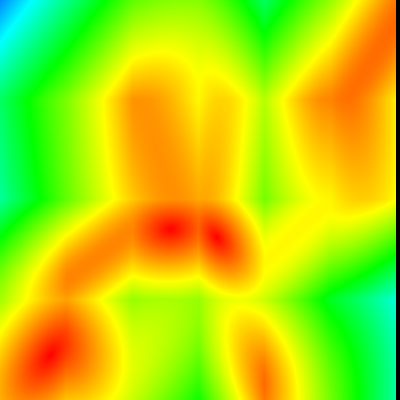
\includegraphics[width=13.0cm]{/tmp/test6.tikz-images/image1.png}};
\draw[line width=0.25000mm, join=round, cap=round, color=000000] (0.00000,0.00000) -- (0.00000,-1.00000);
\draw[line width=0.25000mm, join=round, cap=round, color=000000] (0.16500,0.00000) -- (0.16500,-1.00000);
\draw[line width=0.25000mm, join=round, cap=round, color=000000] (0.33000,0.00000) -- (0.33000,-1.00000);
\draw[line width=0.25000mm, join=round, cap=round, color=000000] (0.49500,0.00000) -- (0.49500,-1.00000);
\draw[line width=0.25000mm, join=round, cap=round, color=000000] (0.66000,0.00000) -- (0.66000,-1.00000);
\draw[line width=0.25000mm, join=round, cap=round, color=000000] (0.82500,0.00000) -- (0.82500,-1.00000);
\draw[line width=0.25000mm, join=round, cap=round, color=000000] (0.99000,0.00000) -- (0.99000,-1.00000);
\draw[line width=0.25000mm, join=round, cap=round, color=000000] (0.00000,0.00000) -- (0.99000,0.00000);
\draw[line width=0.25000mm, join=round, cap=round, color=000000] (0.00000,-0.25000) -- (0.99000,-0.25000);
\draw[line width=0.25000mm, join=round, cap=round, color=000000] (0.00000,-0.50000) -- (0.99000,-0.50000);
\draw[line width=0.25000mm, join=round, cap=round, color=000000] (0.00000,-0.75000) -- (0.99000,-0.75000);
\draw[line width=0.25000mm, join=round, cap=round, color=000000] (0.00000,-1.00000) -- (0.99000,-1.00000);
\end{tikzpicture}
\end{center}
Also there should be some text below. This text block
should also be a not too short, so that there will be a line
break within the paragraph.
\begin{center}
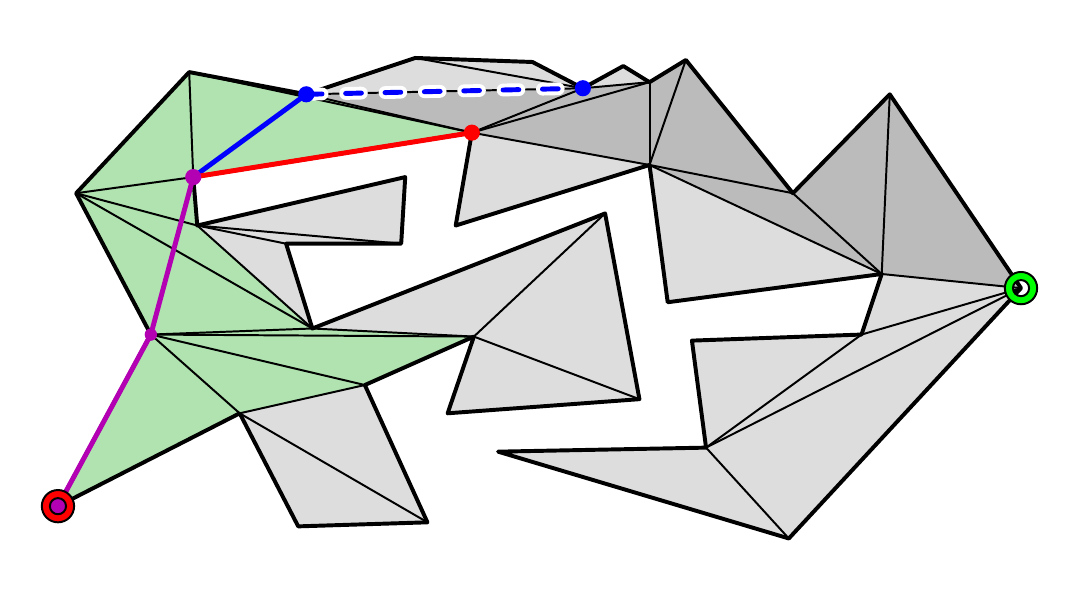
\begin{tikzpicture}[scale=13.0]
\clip (0,0) rectangle (1.000000,-0.528600);
\definecolor{FFFFFF}{rgb}{1.00000,1.00000,1.00000}
\definecolor{DDDDDD}{rgb}{0.86667,0.86667,0.86667}
\definecolor{00FF00}{rgb}{0.00000,1.00000,0.00000}
\definecolor{BBBBBB}{rgb}{0.73333,0.73333,0.73333}
\definecolor{000000}{rgb}{0.00000,0.00000,0.00000}
\definecolor{B200B2}{rgb}{0.69804,0.00000,0.69804}
\definecolor{0000FF}{rgb}{0.00000,0.00000,1.00000}
\definecolor{FF0000}{rgb}{1.00000,0.00000,0.00000}
\clip (0,0) rectangle (1,-1);
\fill[color=FFFFFF] (0.00000, 0.00000) rectangle (1.00000, -0.52860);
\fill[color=DDDDDD, even odd rule] (0.15779,-0.04339) -- (0.04734,-0.16174) -- (0.12032,-0.29980) -- (0.02959,-0.46746) -- (0.20710,-0.37673) -- (0.26430,-0.48718) -- (0.39053,-0.48323) -- (0.32939,-0.34911) -- (0.43590,-0.30178) -- (0.41026,-0.37673) -- (0.59763,-0.36292) -- (0.56410,-0.18146) -- (0.27811,-0.29389) -- (0.25247,-0.21105) -- (0.36489,-0.21105) -- (0.36884,-0.14596) -- (0.16568,-0.19329) -- (0.16174,-0.14596) -- (0.43393,-0.10256) -- (0.41815,-0.19329) -- (0.60750,-0.13412) -- (0.62525,-0.26824) -- (0.83432,-0.24063) -- (0.81460,-0.29980) -- (0.64892,-0.30572) -- (0.66272,-0.41026) -- (0.45957,-0.41420) -- (0.74359,-0.49901) -- (0.97041,-0.25444) -- (0.84221,-0.06509) -- (0.74753,-0.16174) -- (0.64300,-0.03156) -- (0.60750,-0.05325) -- (0.58185,-0.03748) -- (0.54241,-0.05917) -- (0.49310,-0.03353) -- (0.37870,-0.02959) -- (0.27219,-0.06509) -- cycle;
\fill[color=00FF00, opacity=0.20, even odd rule] (0.12032,-0.29980) -- (0.02959,-0.46746) -- (0.20710,-0.37673) -- cycle;
\fill[color=00FF00, opacity=0.20, even odd rule] (0.20710,-0.37673) -- (0.32939,-0.34911) -- (0.12032,-0.29980) -- cycle;
\fill[color=00FF00, opacity=0.20, even odd rule] (0.32939,-0.34911) -- (0.43590,-0.30178) -- (0.12032,-0.29980) -- cycle;
\fill[color=00FF00, opacity=0.20, even odd rule] (0.27811,-0.29389) -- (0.12032,-0.29980) -- (0.43590,-0.30178) -- cycle;
\fill[color=00FF00, opacity=0.20, even odd rule] (0.04734,-0.16174) -- (0.12032,-0.29980) -- (0.27811,-0.29389) -- cycle;
\fill[color=00FF00, opacity=0.20, even odd rule] (0.27811,-0.29389) -- (0.16568,-0.19329) -- (0.04734,-0.16174) -- cycle;
\fill[color=00FF00, opacity=0.20, even odd rule] (0.16568,-0.19329) -- (0.16174,-0.14596) -- (0.04734,-0.16174) -- cycle;
\fill[color=00FF00, opacity=0.20, even odd rule] (0.16174,-0.14596) -- (0.15779,-0.04339) -- (0.04734,-0.16174) -- cycle;
\fill[color=00FF00, opacity=0.20, even odd rule] (0.16174,-0.14596) -- (0.43393,-0.10256) -- (0.15779,-0.04339) -- cycle;
\fill[color=00FF00, opacity=0.20, even odd rule] (0.43393,-0.10256) -- (0.27219,-0.06509) -- (0.15779,-0.04339) -- cycle;
\fill[color=BBBBBB, even odd rule] (0.54241,-0.05917) -- (0.27219,-0.06509) -- (0.43393,-0.10256) -- cycle;
\fill[color=BBBBBB, even odd rule] (0.60750,-0.05325) -- (0.54241,-0.05917) -- (0.43393,-0.10256) -- cycle;
\fill[color=BBBBBB, even odd rule] (0.60750,-0.05325) -- (0.43393,-0.10256) -- (0.60750,-0.13412) -- cycle;
\fill[color=BBBBBB, even odd rule] (0.64300,-0.03156) -- (0.60750,-0.05325) -- (0.60750,-0.13412) -- cycle;
\fill[color=BBBBBB, even odd rule] (0.74753,-0.16174) -- (0.64300,-0.03156) -- (0.60750,-0.13412) -- cycle;
\fill[color=BBBBBB, even odd rule] (0.83432,-0.24063) -- (0.74753,-0.16174) -- (0.60750,-0.13412) -- cycle;
\fill[color=BBBBBB, even odd rule] (0.84221,-0.06509) -- (0.74753,-0.16174) -- (0.83432,-0.24063) -- cycle;
\fill[color=BBBBBB, even odd rule] (0.97041,-0.25444) -- (0.84221,-0.06509) -- (0.83432,-0.24063) -- cycle;
\draw[line width=0.50000mm, join=round, cap=round, color=000000] (0.15779,-0.04339) -- (0.04734,-0.16174) -- (0.12032,-0.29980) -- (0.02959,-0.46746) -- (0.20710,-0.37673) -- (0.26430,-0.48718) -- (0.39053,-0.48323) -- (0.32939,-0.34911) -- (0.43590,-0.30178) -- (0.41026,-0.37673) -- (0.59763,-0.36292) -- (0.56410,-0.18146) -- (0.27811,-0.29389) -- (0.25247,-0.21105) -- (0.36489,-0.21105) -- (0.36884,-0.14596) -- (0.16568,-0.19329) -- (0.16174,-0.14596) -- (0.43393,-0.10256) -- (0.41815,-0.19329) -- (0.60750,-0.13412) -- (0.62525,-0.26824) -- (0.83432,-0.24063) -- (0.81460,-0.29980) -- (0.64892,-0.30572) -- (0.66272,-0.41026) -- (0.45957,-0.41420) -- (0.74359,-0.49901) -- (0.97041,-0.25444) -- (0.84221,-0.06509) -- (0.74753,-0.16174) -- (0.64300,-0.03156) -- (0.60750,-0.05325) -- (0.58185,-0.03748) -- (0.54241,-0.05917) -- (0.49310,-0.03353) -- (0.37870,-0.02959) -- (0.27219,-0.06509) -- cycle;
\draw[line width=0.25000mm, join=round, cap=round, color=000000] (0.54241,-0.05917) -- (0.60750,-0.05325);
\draw[line width=0.25000mm, join=round, cap=round, color=000000] (0.27219,-0.06509) -- (0.54241,-0.05917);
\draw[line width=0.25000mm, join=round, cap=round, color=000000] (0.43393,-0.10256) -- (0.27219,-0.06509);
\draw[line width=0.25000mm, join=round, cap=round, color=000000] (0.60750,-0.13412) -- (0.43393,-0.10256);
\draw[line width=0.25000mm, join=round, cap=round, color=000000] (0.25247,-0.21105) -- (0.16568,-0.19329);
\draw[line width=0.25000mm, join=round, cap=round, color=000000] (0.83432,-0.24063) -- (0.74753,-0.16174);
\draw[line width=0.25000mm, join=round, cap=round, color=000000] (0.12032,-0.29980) -- (0.27811,-0.29389);
\draw[line width=0.25000mm, join=round, cap=round, color=000000] (0.43590,-0.30178) -- (0.12032,-0.29980);
\draw[line width=0.25000mm, join=round, cap=round, color=000000] (0.20710,-0.37673) -- (0.32939,-0.34911);
\draw[line width=0.25000mm, join=round, cap=round, color=000000] (0.83432,-0.24063) -- (0.84221,-0.06509);
\draw[line width=0.25000mm, join=round, cap=round, color=000000] (0.97041,-0.25444) -- (0.83432,-0.24063);
\draw[line width=0.25000mm, join=round, cap=round, color=000000] (0.81460,-0.29980) -- (0.97041,-0.25444);
\draw[line width=0.25000mm, join=round, cap=round, color=000000] (0.66272,-0.41026) -- (0.81460,-0.29980);
\draw[line width=0.25000mm, join=round, cap=round, color=000000] (0.66272,-0.41026) -- (0.97041,-0.25444);
\draw[line width=0.25000mm, join=round, cap=round, color=000000] (0.74359,-0.49901) -- (0.66272,-0.41026);
\draw[line width=0.25000mm, join=round, cap=round, color=000000] (0.43393,-0.10256) -- (0.54241,-0.05917);
\draw[line width=0.25000mm, join=round, cap=round, color=000000] (0.43393,-0.10256) -- (0.60750,-0.05325);
\draw[line width=0.25000mm, join=round, cap=round, color=000000] (0.60750,-0.13412) -- (0.60750,-0.05325);
\draw[line width=0.25000mm, join=round, cap=round, color=000000] (0.60750,-0.13412) -- (0.64300,-0.03156);
\draw[line width=0.25000mm, join=round, cap=round, color=000000] (0.74753,-0.16174) -- (0.60750,-0.13412);
\draw[line width=0.25000mm, join=round, cap=round, color=000000] (0.83432,-0.24063) -- (0.60750,-0.13412);
\draw[line width=0.25000mm, join=round, cap=round, color=000000] (0.36489,-0.21105) -- (0.16568,-0.19329);
\draw[line width=0.25000mm, join=round, cap=round, color=000000] (0.43590,-0.30178) -- (0.27811,-0.29389);
\draw[line width=0.25000mm, join=round, cap=round, color=000000] (0.43590,-0.30178) -- (0.56410,-0.18146);
\draw[line width=0.25000mm, join=round, cap=round, color=000000] (0.59763,-0.36292) -- (0.43590,-0.30178);
\draw[line width=0.25000mm, join=round, cap=round, color=000000] (0.39053,-0.48323) -- (0.20710,-0.37673);
\draw[line width=0.25000mm, join=round, cap=round, color=000000] (0.32939,-0.34911) -- (0.12032,-0.29980);
\draw[line width=0.25000mm, join=round, cap=round, color=000000] (0.20710,-0.37673) -- (0.12032,-0.29980);
\draw[line width=0.25000mm, join=round, cap=round, color=000000] (0.43393,-0.10256) -- (0.15779,-0.04339);
\draw[line width=0.25000mm, join=round, cap=round, color=000000] (0.16174,-0.14596) -- (0.15779,-0.04339);
\draw[line width=0.25000mm, join=round, cap=round, color=000000] (0.04734,-0.16174) -- (0.16174,-0.14596);
\draw[line width=0.25000mm, join=round, cap=round, color=000000] (0.16568,-0.19329) -- (0.04734,-0.16174);
\draw[line width=0.25000mm, join=round, cap=round, color=000000] (0.27811,-0.29389) -- (0.16568,-0.19329);
\draw[line width=0.25000mm, join=round, cap=round, color=000000] (0.27811,-0.29389) -- (0.04734,-0.16174);
\draw[line width=0.25000mm, join=round, cap=round, color=000000] (0.54241,-0.05917) -- (0.37870,-0.02959);
\draw[line width=0.62500mm, join=round, cap=round, color=B200B2] (0.02959,-0.46746) -- (0.12032,-0.29980);
\draw[line width=0.62500mm, join=round, cap=round, color=B200B2] (0.12032,-0.29980) -- (0.12032,-0.29980);
\draw[line width=0.62500mm, join=round, cap=round, color=B200B2] (0.12032,-0.29980) -- (0.16174,-0.14596);
\draw[line width=0.62500mm, join=round, cap=round, color=B200B2] (0.16174,-0.14596) -- (0.16174,-0.14596);
\fill[color=B200B2, even odd rule]  (0.02959,-0.47535) .. controls (0.02523,-0.47535) and (0.02170,-0.47181) .. (0.02170,-0.46746) .. controls (0.02170,-0.46310) and (0.02523,-0.45957) .. (0.02959,-0.45957) .. controls (0.03394,-0.45957) and (0.03748,-0.46310) .. (0.03748,-0.46746) .. controls (0.03748,-0.47181) and (0.03394,-0.47535) .. (0.02959,-0.47535) -- (0.02959,-0.47535) -- cycle;
\fill[color=B200B2, even odd rule]  (0.12032,-0.30572) .. controls (0.11705,-0.30572) and (0.11440,-0.30307) .. (0.11440,-0.29980) .. controls (0.11440,-0.29653) and (0.11705,-0.29389) .. (0.12032,-0.29389) .. controls (0.12358,-0.29389) and (0.12623,-0.29653) .. (0.12623,-0.29980) .. controls (0.12623,-0.30307) and (0.12358,-0.30572) .. (0.12032,-0.30572) -- (0.12032,-0.30572) -- cycle;
\fill[color=B200B2, even odd rule]  (0.12032,-0.30572) .. controls (0.11705,-0.30572) and (0.11440,-0.30307) .. (0.11440,-0.29980) .. controls (0.11440,-0.29653) and (0.11705,-0.29389) .. (0.12032,-0.29389) .. controls (0.12358,-0.29389) and (0.12623,-0.29653) .. (0.12623,-0.29980) .. controls (0.12623,-0.30307) and (0.12358,-0.30572) .. (0.12032,-0.30572) -- (0.12032,-0.30572) -- cycle;
\fill[color=B200B2, even odd rule]  (0.16174,-0.15187) .. controls (0.15847,-0.15187) and (0.15582,-0.14922) .. (0.15582,-0.14596) .. controls (0.15582,-0.14269) and (0.15847,-0.14004) .. (0.16174,-0.14004) .. controls (0.16500,-0.14004) and (0.16765,-0.14269) .. (0.16765,-0.14596) .. controls (0.16765,-0.14922) and (0.16500,-0.15187) .. (0.16174,-0.15187) -- (0.16174,-0.15187) -- cycle;
\draw[line width=0.62500mm, join=round, cap=round, color=0000FF] (0.16174,-0.14596) -- (0.27219,-0.06509);
\draw[line width=0.62500mm, join=round, cap=round, color=FF0000] (0.16174,-0.14596) -- (0.43393,-0.10256);
\draw[line width=1.62500mm, join=round, cap=round, color=FFFFFF, dash pattern=on 2.0mm off 3.0mm, dash phase=0.0] (0.27219,-0.06509) -- (0.54241,-0.05917);
\draw[line width=0.62500mm, join=round, cap=round, color=0000FF, dash pattern=on 2.0mm off 3.0mm, dash phase=0.0] (0.27219,-0.06509) -- (0.54241,-0.05917);
\fill[color=0000FF, even odd rule]  (0.27219,-0.07101) .. controls (0.26892,-0.07101) and (0.26627,-0.06836) .. (0.26627,-0.06509) .. controls (0.26627,-0.06182) and (0.26892,-0.05917) .. (0.27219,-0.05917) .. controls (0.27546,-0.05917) and (0.27811,-0.06182) .. (0.27811,-0.06509) .. controls (0.27811,-0.06836) and (0.27546,-0.07101) .. (0.27219,-0.07101) -- (0.27219,-0.07101) -- cycle;
\fill[color=0000FF, even odd rule]  (0.27219,-0.07298) .. controls (0.26783,-0.07298) and (0.26430,-0.06945) .. (0.26430,-0.06509) .. controls (0.26430,-0.06073) and (0.26783,-0.05720) .. (0.27219,-0.05720) .. controls (0.27655,-0.05720) and (0.28008,-0.06073) .. (0.28008,-0.06509) .. controls (0.28008,-0.06945) and (0.27655,-0.07298) .. (0.27219,-0.07298) -- (0.27219,-0.07298) -- cycle;
\fill[color=FF0000, even odd rule]  (0.43393,-0.10848) .. controls (0.43066,-0.10848) and (0.42801,-0.10583) .. (0.42801,-0.10256) .. controls (0.42801,-0.09930) and (0.43066,-0.09665) .. (0.43393,-0.09665) .. controls (0.43719,-0.09665) and (0.43984,-0.09930) .. (0.43984,-0.10256) .. controls (0.43984,-0.10583) and (0.43719,-0.10848) .. (0.43393,-0.10848) -- (0.43393,-0.10848) -- cycle;
\fill[color=FF0000, even odd rule]  (0.43393,-0.11045) .. controls (0.42957,-0.11045) and (0.42604,-0.10692) .. (0.42604,-0.10256) .. controls (0.42604,-0.09821) and (0.42957,-0.09467) .. (0.43393,-0.09467) .. controls (0.43828,-0.09467) and (0.44181,-0.09821) .. (0.44181,-0.10256) .. controls (0.44181,-0.10692) and (0.43828,-0.11045) .. (0.43393,-0.11045) -- (0.43393,-0.11045) -- cycle;
\fill[color=B200B2, even odd rule]  (0.16174,-0.15385) .. controls (0.15738,-0.15385) and (0.15385,-0.15031) .. (0.15385,-0.14596) .. controls (0.15385,-0.14160) and (0.15738,-0.13807) .. (0.16174,-0.13807) .. controls (0.16609,-0.13807) and (0.16963,-0.14160) .. (0.16963,-0.14596) .. controls (0.16963,-0.15031) and (0.16609,-0.15385) .. (0.16174,-0.15385) -- (0.16174,-0.15385) -- cycle;
\fill[color=0000FF, even odd rule]  (0.54241,-0.06706) .. controls (0.53805,-0.06706) and (0.53452,-0.06353) .. (0.53452,-0.05917) .. controls (0.53452,-0.05481) and (0.53805,-0.05128) .. (0.54241,-0.05128) .. controls (0.54676,-0.05128) and (0.55030,-0.05481) .. (0.55030,-0.05917) .. controls (0.55030,-0.06353) and (0.54676,-0.06706) .. (0.54241,-0.06706) -- (0.54241,-0.06706) -- cycle;
\draw[line width=1.00000mm, join=round, cap=round, color=FF0000]  (0.04142,-0.46746) .. controls (0.04142,-0.46092) and (0.03612,-0.45562) .. (0.02959,-0.45562) .. controls (0.02305,-0.45562) and (0.01775,-0.46092) .. (0.01775,-0.46746) .. controls (0.01775,-0.47399) and (0.02305,-0.47929) .. (0.02959,-0.47929) .. controls (0.03612,-0.47929) and (0.04142,-0.47399) .. (0.04142,-0.46746) -- (0.04142,-0.46746) -- cycle;
\draw[line width=1.00000mm, join=round, cap=round, color=00FF00]  (0.98225,-0.25444) .. controls (0.98225,-0.24790) and (0.97695,-0.24260) .. (0.97041,-0.24260) .. controls (0.96388,-0.24260) and (0.95858,-0.24790) .. (0.95858,-0.25444) .. controls (0.95858,-0.26097) and (0.96388,-0.26627) .. (0.97041,-0.26627) .. controls (0.97695,-0.26627) and (0.98225,-0.26097) .. (0.98225,-0.25444) -- (0.98225,-0.25444) -- cycle;
\draw[line width=0.25000mm, join=round, cap=round, color=000000]  (0.04536,-0.46746) .. controls (0.04536,-0.45874) and (0.03830,-0.45168) .. (0.02959,-0.45168) .. controls (0.02087,-0.45168) and (0.01381,-0.45874) .. (0.01381,-0.46746) .. controls (0.01381,-0.47617) and (0.02087,-0.48323) .. (0.02959,-0.48323) .. controls (0.03830,-0.48323) and (0.04536,-0.47617) .. (0.04536,-0.46746) -- (0.04536,-0.46746) -- cycle;
\draw[line width=0.25000mm, join=round, cap=round, color=000000]  (0.03748,-0.46746) .. controls (0.03748,-0.46310) and (0.03394,-0.45957) .. (0.02959,-0.45957) .. controls (0.02523,-0.45957) and (0.02170,-0.46310) .. (0.02170,-0.46746) .. controls (0.02170,-0.47181) and (0.02523,-0.47535) .. (0.02959,-0.47535) .. controls (0.03394,-0.47535) and (0.03748,-0.47181) .. (0.03748,-0.46746) -- (0.03748,-0.46746) -- cycle;
\draw[line width=0.25000mm, join=round, cap=round, color=000000]  (0.98619,-0.25444) .. controls (0.98619,-0.24572) and (0.97913,-0.23866) .. (0.97041,-0.23866) .. controls (0.96170,-0.23866) and (0.95464,-0.24572) .. (0.95464,-0.25444) .. controls (0.95464,-0.26315) and (0.96170,-0.27022) .. (0.97041,-0.27022) .. controls (0.97913,-0.27022) and (0.98619,-0.26315) .. (0.98619,-0.25444) -- (0.98619,-0.25444) -- cycle;
\draw[line width=0.25000mm, join=round, cap=round, color=000000]  (0.97830,-0.25444) .. controls (0.97830,-0.25008) and (0.97477,-0.24655) .. (0.97041,-0.24655) .. controls (0.96606,-0.24655) and (0.96252,-0.25008) .. (0.96252,-0.25444) .. controls (0.96252,-0.25880) and (0.96606,-0.26233) .. (0.97041,-0.26233) .. controls (0.97477,-0.26233) and (0.97830,-0.25880) .. (0.97830,-0.25444) -- (0.97830,-0.25444) -- cycle;
\end{tikzpicture}
\end{center}
Also there should be some text below. This text block
should also be a not too short, so that there will be a line
break within the paragraph.
\begin{center}
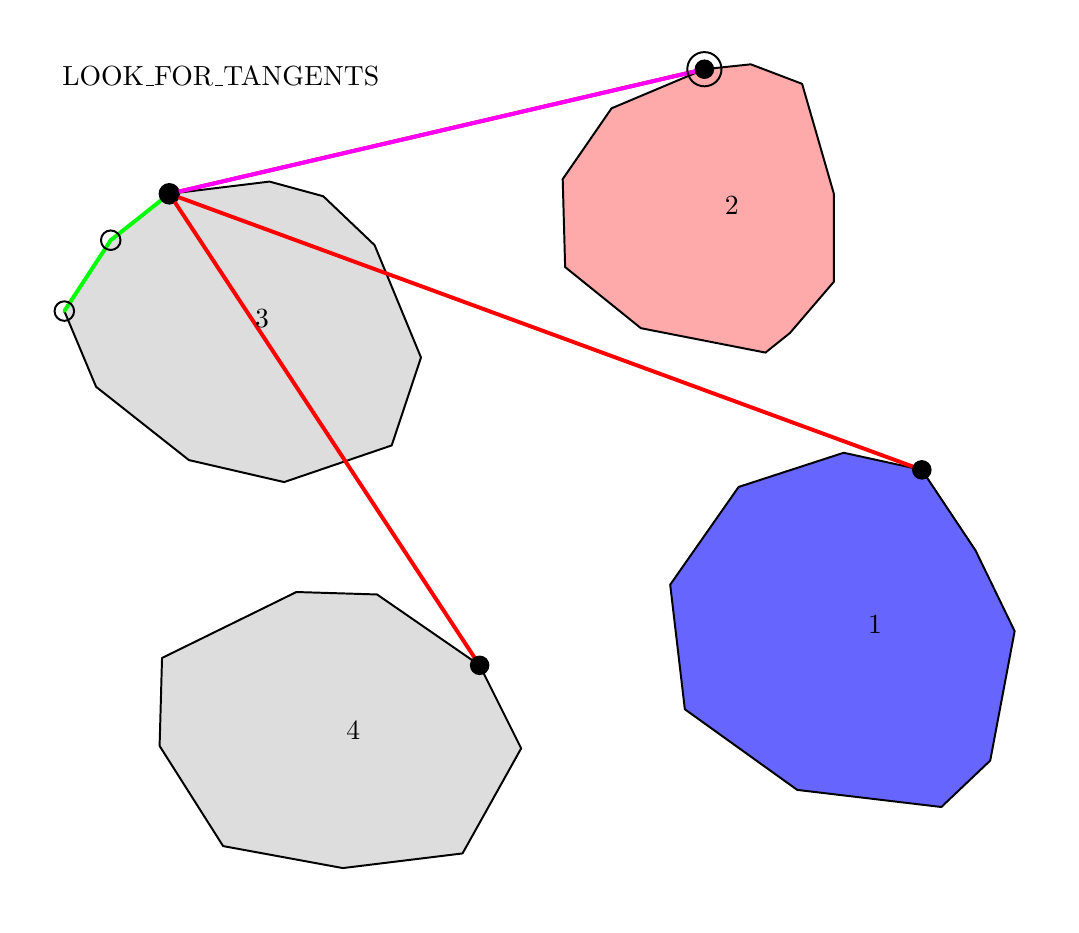
\begin{tikzpicture}[scale=13.0]
\clip (0,0) rectangle (1.000000,-0.856802);
\definecolor{FFFFFF}{rgb}{1.00000,1.00000,1.00000}
\definecolor{000000}{rgb}{0.00000,0.00000,0.00000}
\definecolor{DDDDDD}{rgb}{0.86667,0.86667,0.86667}
\definecolor{6666FF}{rgb}{0.40000,0.40000,1.00000}
\definecolor{FFAAAA}{rgb}{1.00000,0.66667,0.66667}
\definecolor{00FF00}{rgb}{0.00000,1.00000,0.00000}
\definecolor{FF0000}{rgb}{1.00000,0.00000,0.00000}
\definecolor{FF00FF}{rgb}{1.00000,0.00000,1.00000}
\clip (0,0) rectangle (1,-1);
\fill[color=FFFFFF] (0.00000, 0.00000) rectangle (1.00000, -0.85680);
\draw[line width=0.25000mm, join=round, cap=round, color=000000] (0.02387,-0.04773)node[anchor=west] {LOOK\_FOR\_TANGENTS};\fill[color=DDDDDD, even odd rule] (0.66110,-0.04057) -- (0.57041,-0.07876) -- (0.52267,-0.14797) -- (0.52506,-0.23389) -- (0.59905,-0.29356) -- (0.72076,-0.31742) -- (0.74463,-0.29833) -- (0.78759,-0.24821) -- (0.78759,-0.16229) -- (0.75656,-0.05489) -- (0.70644,-0.03580) -- cycle;
\fill[color=DDDDDD, even odd rule] (0.23628,-0.15036) -- (0.13842,-0.16229) -- (0.08115,-0.20764) -- (0.03580,-0.27685) -- (0.06683,-0.35084) -- (0.15752,-0.42243) -- (0.25060,-0.44391) -- (0.35561,-0.40811) -- (0.38425,-0.32220) -- (0.33890,-0.21241) -- (0.28878,-0.16468) -- cycle;
\fill[color=DDDDDD, even odd rule] (0.26253,-0.55131) -- (0.13126,-0.61575) -- (0.12888,-0.70167) -- (0.19093,-0.79952) -- (0.30788,-0.82100) -- (0.42482,-0.80668) -- (0.48210,-0.70406) -- (0.44153,-0.62291) -- (0.34129,-0.55370) -- cycle;
\fill[color=6666FF, even odd rule] (0.79714,-0.41527) -- (0.69451,-0.44869) -- (0.62768,-0.54415) -- (0.64200,-0.66587) -- (0.75179,-0.74463) -- (0.89260,-0.76134) -- (0.94033,-0.71599) -- (0.96420,-0.58950) -- (0.92601,-0.51074) -- (0.87351,-0.43198) -- cycle;
\fill[color=FFAAAA, even odd rule] (0.66110,-0.04057) -- (0.57041,-0.07876) -- (0.52267,-0.14797) -- (0.52506,-0.23389) -- (0.59905,-0.29356) -- (0.72076,-0.31742) -- (0.74463,-0.29833) -- (0.78759,-0.24821) -- (0.78759,-0.16229) -- (0.75656,-0.05489) -- (0.70644,-0.03580) -- cycle;
\draw[line width=0.25000mm, join=round, cap=round, color=000000] (0.79714,-0.41527) -- (0.69451,-0.44869) -- (0.62768,-0.54415) -- (0.64200,-0.66587) -- (0.75179,-0.74463) -- (0.89260,-0.76134) -- (0.94033,-0.71599) -- (0.96420,-0.58950) -- (0.92601,-0.51074) -- (0.87351,-0.43198) -- cycle;
\draw[line width=0.25000mm, join=round, cap=round, color=000000] (0.66110,-0.04057) -- (0.57041,-0.07876) -- (0.52267,-0.14797) -- (0.52506,-0.23389) -- (0.59905,-0.29356) -- (0.72076,-0.31742) -- (0.74463,-0.29833) -- (0.78759,-0.24821) -- (0.78759,-0.16229) -- (0.75656,-0.05489) -- (0.70644,-0.03580) -- cycle;
\draw[line width=0.25000mm, join=round, cap=round, color=000000] (0.23628,-0.15036) -- (0.13842,-0.16229) -- (0.08115,-0.20764) -- (0.03580,-0.27685) -- (0.06683,-0.35084) -- (0.15752,-0.42243) -- (0.25060,-0.44391) -- (0.35561,-0.40811) -- (0.38425,-0.32220) -- (0.33890,-0.21241) -- (0.28878,-0.16468) -- cycle;
\draw[line width=0.25000mm, join=round, cap=round, color=000000] (0.26253,-0.55131) -- (0.13126,-0.61575) -- (0.12888,-0.70167) -- (0.19093,-0.79952) -- (0.30788,-0.82100) -- (0.42482,-0.80668) -- (0.48210,-0.70406) -- (0.44153,-0.62291) -- (0.34129,-0.55370) -- cycle;
\draw[line width=0.50000mm, join=round, cap=round, color=00FF00] (0.03580,-0.27685) -- (0.08115,-0.20764) -- (0.13842,-0.16229);
\draw[line width=0.25000mm, join=round, cap=round, color=000000] (0.03580,-0.27685) circle (0.00955);
\draw[line width=0.25000mm, join=round, cap=round, color=000000] (0.08115,-0.20764) circle (0.00955);
\draw[line width=0.25000mm, join=round, cap=round, color=000000] (0.13842,-0.16229) circle (0.00955);
\draw[line width=0.50000mm, join=round, cap=round, color=FF0000] (0.13842,-0.16229) -- (0.87351,-0.43198);
\draw[line width=0.50000mm, join=round, cap=round, color=FF0000] (0.13842,-0.16229) -- (0.66110,-0.04057);
\draw[line width=0.50000mm, join=round, cap=round, color=FF0000] (0.13842,-0.16229) -- (0.13842,-0.16229);
\draw[line width=0.50000mm, join=round, cap=round, color=FF0000] (0.13842,-0.16229) -- (0.44153,-0.62291);
\draw[line width=0.50000mm, join=round, cap=round, color=FF00FF] (0.13842,-0.16229) -- (0.66110,-0.04057);
\fill[color=000000] (0.87351,-0.43198) circle (0.00955);
\fill[color=000000] (0.66110,-0.04057) circle (0.00955);
\fill[color=000000] (0.13842,-0.16229) circle (0.00955);
\fill[color=000000] (0.44153,-0.62291) circle (0.00955);
\draw[line width=0.25000mm, join=round, cap=round, color=000000] (0.66110,-0.04057) circle (0.01671);
\draw[line width=0.25000mm, join=round, cap=round, color=000000] (0.81098,-0.58282)node[anchor=west] {1};\draw[line width=0.25000mm, join=round, cap=round, color=000000] (0.67108,-0.17379)node[anchor=west] {2};\draw[line width=0.25000mm, join=round, cap=round, color=000000] (0.21219,-0.28379)node[anchor=west] {3};\draw[line width=0.25000mm, join=round, cap=round, color=000000] (0.30125,-0.68629)node[anchor=west] {4};\end{tikzpicture}
\end{center}
Also there should be some text below. This text block
should also be a not too short, so that there will be a line
break within the paragraph.
\begin{center}
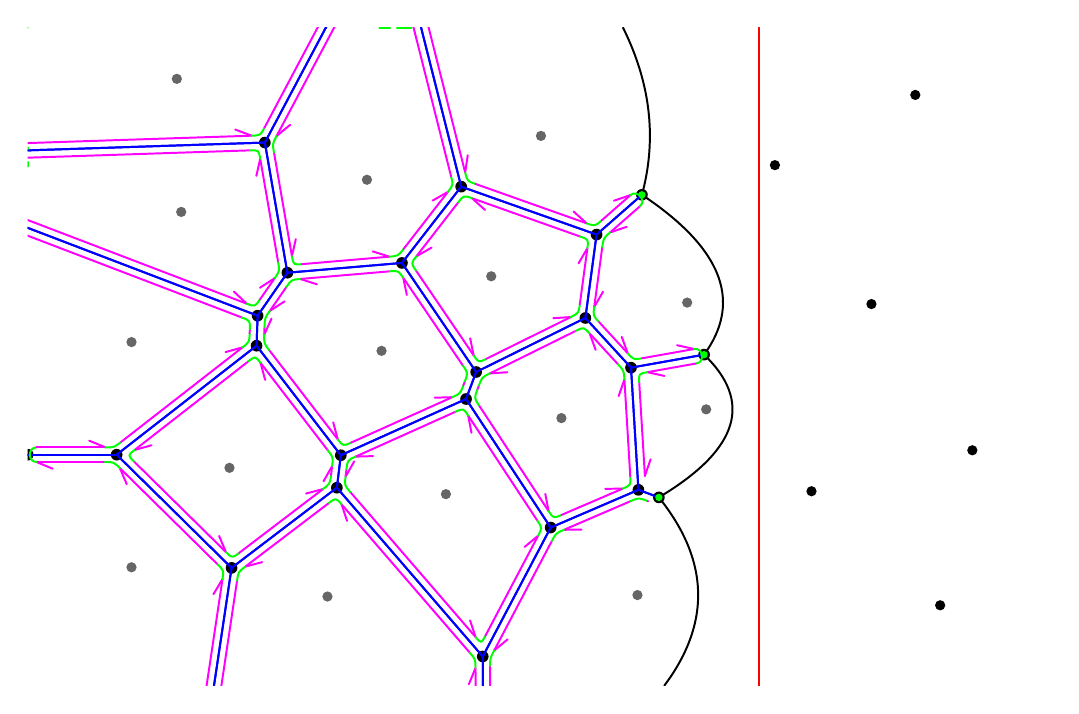
\begin{tikzpicture}[scale=13.0]
\clip (0,0) rectangle (1.000000,-0.642857);
\definecolor{FFFFFF}{rgb}{1.00000,1.00000,1.00000}
\definecolor{000000}{rgb}{0.00000,0.00000,0.00000}
\definecolor{0000FF}{rgb}{0.00000,0.00000,1.00000}
\definecolor{FF00FF}{rgb}{1.00000,0.00000,1.00000}
\definecolor{00FF00}{rgb}{0.00000,1.00000,0.00000}
\definecolor{666666}{rgb}{0.40000,0.40000,0.40000}
\definecolor{FF0000}{rgb}{1.00000,0.00000,0.00000}
\clip (0,0) rectangle (1,-1);
\fill[color=FFFFFF] (0.00000, 0.00000) rectangle (1.00000, -0.64286);
\fill[color=FFFFFF] (0.00000, 0.00000) rectangle (1.14286, -0.71429);
\fill[color=000000] (0.08694,-0.41714) circle (0.00571);
\fill[color=000000] (0.00000,-0.41714) circle (0.00571);
\fill[color=000000] (-39.98715,6.72939) circle (0.00571);
\fill[color=000000] (-0.18235,-0.12589) circle (0.00571);
\fill[color=000000] (0.22463,-0.28136) circle (0.00571);
\fill[color=000000] (0.23170,-0.11224) circle (0.00571);
\fill[color=000000] (0.19919,-0.52774) circle (0.00571);
\fill[color=000000] (0.22360,-0.31068) circle (0.00571);
\fill[color=000000] (0.10893,-1.13245) circle (0.00571);
\fill[color=000000] (0.30206,-0.44941) circle (0.00571);
\fill[color=000000] (0.25373,-0.23939) circle (0.00571);
\fill[color=000000] (0.35439,0.11893) circle (0.00571);
\fill[color=000000] (0.30592,-0.41769) circle (0.00571);
\fill[color=000000] (0.36565,-0.22983) circle (0.00571);
\fill[color=000000] (0.42826,-0.36276) circle (0.00571);
\fill[color=000000] (0.43812,-0.33640) circle (0.00571);
\fill[color=000000] (0.42353,-0.15530) circle (0.00571);
\fill[color=000000] (0.55577,-0.20213) circle (0.00571);
\fill[color=000000] (0.51092,-0.48834) circle (0.00571);
\fill[color=000000] (0.44457,-0.61431) circle (0.00571);
\fill[color=000000] (0.44533,-0.77727) circle (0.00571);
\fill[color=000000] (0.36914,0.21307) circle (0.00571);
\fill[color=000000] (0.54483,-0.28360) circle (0.00571);
\fill[color=000000] (0.58942,-0.33214) circle (0.00571);
\fill[color=000000] (0.59665,-0.45149) circle (0.00571);
\fill[color=000000] (0.60008,-0.16327) circle (0.00571);
\fill[color=000000] (0.66081,-0.31942) circle (0.00571);
\fill[color=000000] (0.61662,-0.45888) circle (0.00571);
\draw[line width=0.25000mm, join=round, cap=round, color=0000FF] (0.08694,-0.41714) -- (0.00000,-0.41714);
\draw[line width=0.25000mm, join=round, cap=round, color=0000FF] (0.00000,-0.41714) -- (0.08694,-0.41714);
\draw[line width=0.25000mm, join=round, cap=round, color=0000FF] (-39.98715,6.72939) -- (-0.18235,-0.12589);
\draw[line width=0.25000mm, join=round, cap=round, color=0000FF] (-0.18235,-0.12589) -- (-39.98715,6.72939);
\draw[line width=0.25000mm, join=round, cap=round, color=0000FF] (-0.18235,-0.12589) -- (0.22463,-0.28136);
\draw[line width=0.25000mm, join=round, cap=round, color=0000FF] (0.22463,-0.28136) -- (-0.18235,-0.12589);
\draw[line width=0.25000mm, join=round, cap=round, color=0000FF] (0.23170,-0.11224) -- (-0.18235,-0.12589);
\draw[line width=0.25000mm, join=round, cap=round, color=0000FF] (-0.18235,-0.12589) -- (0.23170,-0.11224);
\draw[line width=0.25000mm, join=round, cap=round, color=0000FF] (0.08694,-0.41714) -- (0.19919,-0.52774);
\draw[line width=0.25000mm, join=round, cap=round, color=0000FF] (0.19919,-0.52774) -- (0.08694,-0.41714);
\draw[line width=0.25000mm, join=round, cap=round, color=0000FF] (0.22360,-0.31068) -- (0.08694,-0.41714);
\draw[line width=0.25000mm, join=round, cap=round, color=0000FF] (0.08694,-0.41714) -- (0.22360,-0.31068);
\draw[line width=0.25000mm, join=round, cap=round, color=0000FF] (0.19919,-0.52774) -- (0.10893,-1.13245);
\draw[line width=0.25000mm, join=round, cap=round, color=0000FF] (0.10893,-1.13245) -- (0.19919,-0.52774);
\draw[line width=0.25000mm, join=round, cap=round, color=0000FF] (0.30206,-0.44941) -- (0.19919,-0.52774);
\draw[line width=0.25000mm, join=round, cap=round, color=0000FF] (0.19919,-0.52774) -- (0.30206,-0.44941);
\draw[line width=0.25000mm, join=round, cap=round, color=0000FF] (0.23170,-0.11224) -- (0.25373,-0.23939);
\draw[line width=0.25000mm, join=round, cap=round, color=0000FF] (0.25373,-0.23939) -- (0.23170,-0.11224);
\draw[line width=0.25000mm, join=round, cap=round, color=0000FF] (0.35439,0.11893) -- (0.23170,-0.11224);
\draw[line width=0.25000mm, join=round, cap=round, color=0000FF] (0.23170,-0.11224) -- (0.35439,0.11893);
\draw[line width=0.25000mm, join=round, cap=round, color=0000FF] (0.22360,-0.31068) -- (0.30592,-0.41769);
\draw[line width=0.25000mm, join=round, cap=round, color=0000FF] (0.30592,-0.41769) -- (0.22360,-0.31068);
\draw[line width=0.25000mm, join=round, cap=round, color=0000FF] (0.22463,-0.28136) -- (0.22360,-0.31068);
\draw[line width=0.25000mm, join=round, cap=round, color=0000FF] (0.22360,-0.31068) -- (0.22463,-0.28136);
\draw[line width=0.25000mm, join=round, cap=round, color=0000FF] (0.25373,-0.23939) -- (0.22463,-0.28136);
\draw[line width=0.25000mm, join=round, cap=round, color=0000FF] (0.22463,-0.28136) -- (0.25373,-0.23939);
\draw[line width=0.25000mm, join=round, cap=round, color=0000FF] (0.36565,-0.22983) -- (0.25373,-0.23939);
\draw[line width=0.25000mm, join=round, cap=round, color=0000FF] (0.25373,-0.23939) -- (0.36565,-0.22983);
\draw[line width=0.25000mm, join=round, cap=round, color=0000FF] (0.30206,-0.44941) -- (0.44457,-0.61431);
\draw[line width=0.25000mm, join=round, cap=round, color=0000FF] (0.44457,-0.61431) -- (0.30206,-0.44941);
\draw[line width=0.25000mm, join=round, cap=round, color=0000FF] (0.30592,-0.41769) -- (0.30206,-0.44941);
\draw[line width=0.25000mm, join=round, cap=round, color=0000FF] (0.30206,-0.44941) -- (0.30592,-0.41769);
\draw[line width=0.25000mm, join=round, cap=round, color=0000FF] (0.42826,-0.36276) -- (0.30592,-0.41769);
\draw[line width=0.25000mm, join=round, cap=round, color=0000FF] (0.30592,-0.41769) -- (0.42826,-0.36276);
\draw[line width=0.25000mm, join=round, cap=round, color=0000FF] (0.36565,-0.22983) -- (0.43812,-0.33640);
\draw[line width=0.25000mm, join=round, cap=round, color=0000FF] (0.43812,-0.33640) -- (0.36565,-0.22983);
\draw[line width=0.25000mm, join=round, cap=round, color=0000FF] (0.42353,-0.15530) -- (0.36565,-0.22983);
\draw[line width=0.25000mm, join=round, cap=round, color=0000FF] (0.36565,-0.22983) -- (0.42353,-0.15530);
\draw[line width=0.25000mm, join=round, cap=round, color=0000FF] (0.35439,0.11893) -- (0.42353,-0.15530);
\draw[line width=0.25000mm, join=round, cap=round, color=0000FF] (0.42353,-0.15530) -- (0.35439,0.11893);
\draw[line width=0.25000mm, join=round, cap=round, color=0000FF] (0.55577,-0.20213) -- (0.42353,-0.15530);
\draw[line width=0.25000mm, join=round, cap=round, color=0000FF] (0.42353,-0.15530) -- (0.55577,-0.20213);
\draw[line width=0.25000mm, join=round, cap=round, color=0000FF] (0.42826,-0.36276) -- (0.51092,-0.48834);
\draw[line width=0.25000mm, join=round, cap=round, color=0000FF] (0.51092,-0.48834) -- (0.42826,-0.36276);
\draw[line width=0.25000mm, join=round, cap=round, color=0000FF] (0.43812,-0.33640) -- (0.42826,-0.36276);
\draw[line width=0.25000mm, join=round, cap=round, color=0000FF] (0.42826,-0.36276) -- (0.43812,-0.33640);
\draw[line width=0.25000mm, join=round, cap=round, color=0000FF] (0.54483,-0.28360) -- (0.43812,-0.33640);
\draw[line width=0.25000mm, join=round, cap=round, color=0000FF] (0.43812,-0.33640) -- (0.54483,-0.28360);
\draw[line width=0.25000mm, join=round, cap=round, color=0000FF] (0.51092,-0.48834) -- (0.44457,-0.61431);
\draw[line width=0.25000mm, join=round, cap=round, color=0000FF] (0.44457,-0.61431) -- (0.51092,-0.48834);
\draw[line width=0.25000mm, join=round, cap=round, color=0000FF] (0.44533,-0.77727) -- (0.44457,-0.61431);
\draw[line width=0.25000mm, join=round, cap=round, color=0000FF] (0.44457,-0.61431) -- (0.44533,-0.77727);
\draw[line width=0.25000mm, join=round, cap=round, color=0000FF] (0.59665,-0.45149) -- (0.51092,-0.48834);
\draw[line width=0.25000mm, join=round, cap=round, color=0000FF] (0.51092,-0.48834) -- (0.59665,-0.45149);
\draw[line width=0.25000mm, join=round, cap=round, color=0000FF] (0.36914,0.21307) -- (0.35439,0.11893);
\draw[line width=0.25000mm, join=round, cap=round, color=0000FF] (0.35439,0.11893) -- (0.36914,0.21307);
\draw[line width=0.25000mm, join=round, cap=round, color=0000FF] (0.55577,-0.20213) -- (0.54483,-0.28360);
\draw[line width=0.25000mm, join=round, cap=round, color=0000FF] (0.54483,-0.28360) -- (0.55577,-0.20213);
\draw[line width=0.25000mm, join=round, cap=round, color=0000FF] (0.58942,-0.33214) -- (0.54483,-0.28360);
\draw[line width=0.25000mm, join=round, cap=round, color=0000FF] (0.54483,-0.28360) -- (0.58942,-0.33214);
\draw[line width=0.25000mm, join=round, cap=round, color=0000FF] (0.58942,-0.33214) -- (0.59665,-0.45149);
\draw[line width=0.25000mm, join=round, cap=round, color=0000FF] (0.59665,-0.45149) -- (0.58942,-0.33214);
\draw[line width=0.25000mm, join=round, cap=round, color=0000FF] (0.60008,-0.16327) -- (0.55577,-0.20213);
\draw[line width=0.25000mm, join=round, cap=round, color=0000FF] (0.55577,-0.20213) -- (0.60008,-0.16327);
\draw[line width=0.25000mm, join=round, cap=round, color=0000FF] (0.66081,-0.31942) -- (0.58942,-0.33214);
\draw[line width=0.25000mm, join=round, cap=round, color=0000FF] (0.58942,-0.33214) -- (0.66081,-0.31942);
\draw[line width=0.25000mm, join=round, cap=round, color=0000FF] (0.61662,-0.45888) -- (0.59665,-0.45149);
\draw[line width=0.25000mm, join=round, cap=round, color=0000FF] (0.59665,-0.45149) -- (0.61662,-0.45888);
\draw[line width=0.25000mm, join=round, cap=round, color=FF00FF] (0.07544,-0.42429) -- (0.00857,-0.42429);
\draw[line width=0.25000mm, join=round, cap=round, color=FF00FF] (0.00857,-0.42429) -- (0.02441,-0.43085);
\draw[line width=0.25000mm, join=round, cap=round, color=00FF00]  (0.00857,-0.42429) .. controls (0.00442,-0.42429) and (0.00228,-0.42093) .. (0.00215,-0.41748) .. controls (0.00201,-0.41380) and (0.00415,-0.41000) .. (0.00857,-0.41000);
\draw[line width=0.25000mm, join=round, cap=round, color=FF00FF] (0.00857,-0.41000) -- (0.07591,-0.41000);
\draw[line width=0.25000mm, join=round, cap=round, color=FF00FF] (0.07591,-0.41000) -- (0.06008,-0.40344);
\draw[line width=0.25000mm, join=round, cap=round, color=00FF00]  (0.07591,-0.41000) .. controls (0.08449,-0.41000) and (0.08449,-0.41000) .. (0.09125,-0.40473);
\draw[line width=0.25000mm, join=round, cap=round, color=FF00FF] (-39.97749,6.73497) -- (-0.19030,-0.11727);
\draw[line width=0.25000mm, join=round, cap=round, color=FF00FF] (-0.19030,-0.11727) -- (-0.20479,-0.10811);
\draw[line width=0.25000mm, join=round, cap=round, color=00FF00]  (0.00000,-0.11727) -- (0.00000,-0.11844);
\draw[line width=0.25000mm, join=round, cap=round, color=FF00FF] (-0.19269,-0.13135) -- (-39.97991,6.72089);
\draw[line width=0.25000mm, join=round, cap=round, color=FF00FF] (-39.97991,6.72089) -- (-39.96542,6.71174);
\draw[line width=0.25000mm, join=round, cap=round, color=00FF00]  (0.00000,0.00000) -- (0.00000,0.00000);
\draw[line width=0.25000mm, join=round, cap=round, color=FF00FF] (-0.13869,-0.13492) -- (0.21394,-0.26963);
\draw[line width=0.25000mm, join=round, cap=round, color=FF00FF] (0.21394,-0.26963) -- (0.20149,-0.25785);
\draw[line width=0.25000mm, join=round, cap=round, color=00FF00]  (0.21394,-0.26963) .. controls (0.22195,-0.27269) and (0.22195,-0.27269) .. (0.22683,-0.26564);
\draw[line width=0.25000mm, join=round, cap=round, color=FF00FF] (0.20930,-0.28315) -- (-0.17624,-0.13587);
\draw[line width=0.25000mm, join=round, cap=round, color=FF00FF] (-0.17624,-0.13587) -- (-0.16378,-0.14765);
\draw[line width=0.25000mm, join=round, cap=round, color=00FF00]  (0.00000,-0.13587) -- (0.00000,-0.13135);
\draw[line width=0.25000mm, join=round, cap=round, color=FF00FF] (0.21715,-0.11986) -- (-0.13813,-0.13157);
\draw[line width=0.25000mm, join=round, cap=round, color=FF00FF] (-0.13813,-0.13157) -- (-0.12209,-0.13761);
\draw[line width=0.25000mm, join=round, cap=round, color=00FF00]  (0.00000,-0.13157) -- (0.00000,-0.13492);
\draw[line width=0.25000mm, join=round, cap=round, color=FF00FF] (-0.17328,-0.11844) -- (0.21876,-0.10552);
\draw[line width=0.25000mm, join=round, cap=round, color=FF00FF] (0.21876,-0.10552) -- (0.20272,-0.09948);
\draw[line width=0.25000mm, join=round, cap=round, color=00FF00]  (0.21876,-0.10552) .. controls (0.22733,-0.10523) and (0.22733,-0.10523) .. (0.23135,-0.09766);
\draw[line width=0.25000mm, join=round, cap=round, color=FF00FF] (0.10386,-0.42379) -- (0.19368,-0.51229);
\draw[line width=0.25000mm, join=round, cap=round, color=FF00FF] (0.19368,-0.51229) -- (0.18700,-0.49650);
\draw[line width=0.25000mm, join=round, cap=round, color=00FF00]  (0.19368,-0.51229) .. controls (0.19979,-0.51830) and (0.19979,-0.51830) .. (0.20661,-0.51311);
\draw[line width=0.25000mm, join=round, cap=round, color=FF00FF] (0.18548,-0.52426) -- (0.09012,-0.43030);
\draw[line width=0.25000mm, join=round, cap=round, color=FF00FF] (0.09012,-0.43030) -- (0.09680,-0.44609);
\draw[line width=0.25000mm, join=round, cap=round, color=00FF00]  (0.09012,-0.43030) .. controls (0.08401,-0.42429) and (0.08401,-0.42429) .. (0.07544,-0.42429);
\draw[line width=0.25000mm, join=round, cap=round, color=FF00FF] (0.21556,-0.32600) -- (0.10452,-0.41250);
\draw[line width=0.25000mm, join=round, cap=round, color=FF00FF] (0.10452,-0.41250) -- (0.12104,-0.40795);
\draw[line width=0.25000mm, join=round, cap=round, color=00FF00]  (0.10452,-0.41250) .. controls (0.09776,-0.41777) and (0.09776,-0.41777) .. (0.10386,-0.42379);
\draw[line width=0.25000mm, join=round, cap=round, color=FF00FF] (0.09125,-0.40473) -- (0.20981,-0.31236);
\draw[line width=0.25000mm, join=round, cap=round, color=FF00FF] (0.20981,-0.31236) -- (0.19329,-0.31692);
\draw[line width=0.25000mm, join=round, cap=round, color=00FF00]  (0.20981,-0.31236) .. controls (0.21658,-0.30709) and (0.21658,-0.30709) .. (0.21688,-0.29853);
\draw[line width=0.25000mm, join=round, cap=round, color=FF00FF] (0.20456,-0.54014) -- (0.11726,-1.12503);
\draw[line width=0.25000mm, join=round, cap=round, color=FF00FF] (0.11726,-1.12503) -- (0.12609,-1.11033);
\draw[line width=0.25000mm, join=round, cap=round, color=00FF00]  (0.11726,-1.00000) -- (0.10313,-1.00000);
\draw[line width=0.25000mm, join=round, cap=round, color=FF00FF] (0.10313,-1.12292) -- (0.19032,-0.53875);
\draw[line width=0.25000mm, join=round, cap=round, color=FF00FF] (0.19032,-0.53875) -- (0.18149,-0.55345);
\draw[line width=0.25000mm, join=round, cap=round, color=00FF00]  (0.19032,-0.53875) .. controls (0.19159,-0.53028) and (0.19159,-0.53028) .. (0.18548,-0.52426);
\draw[line width=0.25000mm, join=round, cap=round, color=FF00FF] (0.29423,-0.46436) -- (0.21264,-0.52647);
\draw[line width=0.25000mm, join=round, cap=round, color=FF00FF] (0.21264,-0.52647) -- (0.22922,-0.52210);
\draw[line width=0.25000mm, join=round, cap=round, color=00FF00]  (0.21264,-0.52647) .. controls (0.20582,-0.53166) and (0.20582,-0.53166) .. (0.20456,-0.54014);
\draw[line width=0.25000mm, join=round, cap=round, color=FF00FF] (0.20661,-0.51311) -- (0.28851,-0.45075);
\draw[line width=0.25000mm, join=round, cap=round, color=FF00FF] (0.28851,-0.45075) -- (0.27194,-0.45512);
\draw[line width=0.25000mm, join=round, cap=round, color=00FF00]  (0.28851,-0.45075) .. controls (0.29533,-0.44556) and (0.29533,-0.44556) .. (0.29637,-0.43705);
\draw[line width=0.25000mm, join=round, cap=round, color=FF00FF] (0.24062,-0.12187) -- (0.25818,-0.22327);
\draw[line width=0.25000mm, join=round, cap=round, color=FF00FF] (0.25818,-0.22327) -- (0.26194,-0.20655);
\draw[line width=0.25000mm, join=round, cap=round, color=00FF00]  (0.25818,-0.22327) .. controls (0.25965,-0.23172) and (0.25965,-0.23172) .. (0.26819,-0.23099);
\draw[line width=0.25000mm, join=round, cap=round, color=FF00FF] (0.24472,-0.22928) -- (0.22718,-0.12803);
\draw[line width=0.25000mm, join=round, cap=round, color=FF00FF] (0.22718,-0.12803) -- (0.22342,-0.14475);
\draw[line width=0.25000mm, join=round, cap=round, color=00FF00]  (0.22718,-0.12803) .. controls (0.22572,-0.11958) and (0.22572,-0.11958) .. (0.21715,-0.11986);
\draw[line width=0.25000mm, join=round, cap=round, color=FF00FF] (0.34798,0.09162) -- (0.24317,-0.10585);
\draw[line width=0.25000mm, join=round, cap=round, color=FF00FF] (0.24317,-0.10585) -- (0.25639,-0.09494);
\draw[line width=0.25000mm, join=round, cap=round, color=00FF00]  (0.24317,-0.10585) .. controls (0.23915,-0.11343) and (0.23915,-0.11343) .. (0.24062,-0.12187);
\draw[line width=0.25000mm, join=round, cap=round, color=FF00FF] (0.23135,-0.09766) -- (0.34350,0.11365);
\draw[line width=0.25000mm, join=round, cap=round, color=FF00FF] (0.34350,0.11365) -- (0.33028,0.10273);
\draw[line width=0.25000mm, join=round, cap=round, color=00FF00]  (0.34350,0.00000) -- (0.34885,0.00000);
\draw[line width=0.25000mm, join=round, cap=round, color=FF00FF] (0.23605,-0.31515) -- (0.30291,-0.40207);
\draw[line width=0.25000mm, join=round, cap=round, color=FF00FF] (0.30291,-0.40207) -- (0.29846,-0.38552);
\draw[line width=0.25000mm, join=round, cap=round, color=00FF00]  (0.30291,-0.40207) .. controls (0.30814,-0.40887) and (0.30814,-0.40887) .. (0.31596,-0.40536);
\draw[line width=0.25000mm, join=round, cap=round, color=FF00FF] (0.29325,-0.41294) -- (0.22754,-0.32752);
\draw[line width=0.25000mm, join=round, cap=round, color=FF00FF] (0.22754,-0.32752) -- (0.23200,-0.34408);
\draw[line width=0.25000mm, join=round, cap=round, color=00FF00]  (0.22754,-0.32752) .. controls (0.22232,-0.32073) and (0.22232,-0.32073) .. (0.21556,-0.32600);
\draw[line width=0.25000mm, join=round, cap=round, color=FF00FF] (0.23139,-0.29227) -- (0.23113,-0.29979);
\draw[line width=0.25000mm, join=round, cap=round, color=FF00FF] (0.23113,-0.29979) -- (0.23824,-0.28419);
\draw[line width=0.25000mm, join=round, cap=round, color=00FF00]  (0.23113,-0.29979) .. controls (0.23083,-0.30836) and (0.23083,-0.30836) .. (0.23605,-0.31515);
\draw[line width=0.25000mm, join=round, cap=round, color=FF00FF] (0.21688,-0.29853) -- (0.21701,-0.29478);
\draw[line width=0.25000mm, join=round, cap=round, color=00FF00]  (0.21701,-0.29478) .. controls (0.21731,-0.28621) and (0.21731,-0.28621) .. (0.20930,-0.28315);
\draw[line width=0.25000mm, join=round, cap=round, color=FF00FF] (0.25280,-0.25327) -- (0.23658,-0.27666);
\draw[line width=0.25000mm, join=round, cap=round, color=FF00FF] (0.23658,-0.27666) -- (0.25099,-0.26738);
\draw[line width=0.25000mm, join=round, cap=round, color=00FF00]  (0.23658,-0.27666) .. controls (0.23169,-0.28370) and (0.23169,-0.28370) .. (0.23139,-0.29227);
\draw[line width=0.25000mm, join=round, cap=round, color=FF00FF] (0.22683,-0.26564) -- (0.24130,-0.24477);
\draw[line width=0.25000mm, join=round, cap=round, color=FF00FF] (0.24130,-0.24477) -- (0.22689,-0.25405);
\draw[line width=0.25000mm, join=round, cap=round, color=00FF00]  (0.24130,-0.24477) .. controls (0.24619,-0.23773) and (0.24619,-0.23773) .. (0.24472,-0.22928);
\draw[line width=0.25000mm, join=round, cap=round, color=FF00FF] (0.35356,-0.23803) -- (0.26622,-0.24550);
\draw[line width=0.25000mm, join=round, cap=round, color=FF00FF] (0.26622,-0.24550) -- (0.28256,-0.25068);
\draw[line width=0.25000mm, join=round, cap=round, color=00FF00]  (0.26622,-0.24550) .. controls (0.25768,-0.24623) and (0.25768,-0.24623) .. (0.25280,-0.25327);
\draw[line width=0.25000mm, join=round, cap=round, color=FF00FF] (0.26819,-0.23099) -- (0.35339,-0.22371);
\draw[line width=0.25000mm, join=round, cap=round, color=FF00FF] (0.35339,-0.22371) -- (0.33705,-0.21852);
\draw[line width=0.25000mm, join=round, cap=round, color=00FF00]  (0.35339,-0.22371) .. controls (0.36193,-0.22298) and (0.36193,-0.22298) .. (0.36719,-0.21621);
\draw[line width=0.25000mm, join=round, cap=round, color=FF00FF] (0.31514,-0.45362) -- (0.43752,-0.59524);
\draw[line width=0.25000mm, join=round, cap=round, color=FF00FF] (0.43752,-0.59524) -- (0.43213,-0.57896);
\draw[line width=0.25000mm, join=round, cap=round, color=00FF00]  (0.43752,-0.59524) .. controls (0.44312,-0.60172) and (0.44312,-0.60172) .. (0.44712,-0.59414);
\draw[line width=0.25000mm, join=round, cap=round, color=FF00FF] (0.43183,-0.61050) -- (0.30665,-0.46565);
\draw[line width=0.25000mm, join=round, cap=round, color=FF00FF] (0.30665,-0.46565) -- (0.31204,-0.48192);
\draw[line width=0.25000mm, join=round, cap=round, color=00FF00]  (0.30665,-0.46565) .. controls (0.30105,-0.45916) and (0.30105,-0.45916) .. (0.29423,-0.46436);
\draw[line width=0.25000mm, join=round, cap=round, color=FF00FF] (0.31149,-0.43107) -- (0.31057,-0.43863);
\draw[line width=0.25000mm, join=round, cap=round, color=FF00FF] (0.31057,-0.43863) -- (0.31899,-0.42370);
\draw[line width=0.25000mm, join=round, cap=round, color=00FF00]  (0.31057,-0.43863) .. controls (0.30953,-0.44714) and (0.30953,-0.44714) .. (0.31514,-0.45362);
\draw[line width=0.25000mm, join=round, cap=round, color=FF00FF] (0.29637,-0.43705) -- (0.29744,-0.42824);
\draw[line width=0.25000mm, join=round, cap=round, color=FF00FF] (0.29744,-0.42824) -- (0.28901,-0.44317);
\draw[line width=0.25000mm, join=round, cap=round, color=00FF00]  (0.29744,-0.42824) .. controls (0.29847,-0.41973) and (0.29847,-0.41973) .. (0.29325,-0.41294);
\draw[line width=0.25000mm, join=round, cap=round, color=FF00FF] (0.41782,-0.37528) -- (0.32034,-0.41905);
\draw[line width=0.25000mm, join=round, cap=round, color=FF00FF] (0.32034,-0.41905) -- (0.33748,-0.41854);
\draw[line width=0.25000mm, join=round, cap=round, color=00FF00]  (0.32034,-0.41905) .. controls (0.31252,-0.42256) and (0.31252,-0.42256) .. (0.31149,-0.43107);
\draw[line width=0.25000mm, join=round, cap=round, color=FF00FF] (0.31596,-0.40535) -- (0.41480,-0.36098);
\draw[line width=0.25000mm, join=round, cap=round, color=FF00FF] (0.41480,-0.36098) -- (0.39766,-0.36148);
\draw[line width=0.25000mm, join=round, cap=round, color=00FF00]  (0.41480,-0.36098) .. controls (0.42262,-0.35747) and (0.42262,-0.35747) .. (0.42562,-0.34944);
\draw[line width=0.25000mm, join=round, cap=round, color=FF00FF] (0.37930,-0.23719) -- (0.43571,-0.32015);
\draw[line width=0.25000mm, join=round, cap=round, color=FF00FF] (0.43571,-0.32015) -- (0.43223,-0.30337);
\draw[line width=0.25000mm, join=round, cap=round, color=00FF00]  (0.43571,-0.32015) .. controls (0.44053,-0.32724) and (0.44053,-0.32724) .. (0.44821,-0.32344);
\draw[line width=0.25000mm, join=round, cap=round, color=FF00FF] (0.42532,-0.33027) -- (0.36692,-0.24439);
\draw[line width=0.25000mm, join=round, cap=round, color=FF00FF] (0.36692,-0.24439) -- (0.37040,-0.26117);
\draw[line width=0.25000mm, join=round, cap=round, color=00FF00]  (0.36692,-0.24439) .. controls (0.36210,-0.23730) and (0.36210,-0.23730) .. (0.35356,-0.23803);
\draw[line width=0.25000mm, join=round, cap=round, color=FF00FF] (0.42075,-0.17052) -- (0.37974,-0.22334);
\draw[line width=0.25000mm, join=round, cap=round, color=FF00FF] (0.37974,-0.22334) -- (0.39463,-0.21485);
\draw[line width=0.25000mm, join=round, cap=round, color=00FF00]  (0.37974,-0.22334) .. controls (0.37448,-0.23011) and (0.37448,-0.23011) .. (0.37930,-0.23719);
\draw[line width=0.25000mm, join=round, cap=round, color=FF00FF] (0.36719,-0.21621) -- (0.41049,-0.16044);
\draw[line width=0.25000mm, join=round, cap=round, color=FF00FF] (0.41049,-0.16044) -- (0.39560,-0.16892);
\draw[line width=0.25000mm, join=round, cap=round, color=00FF00]  (0.41049,-0.16044) .. controls (0.41575,-0.15367) and (0.41575,-0.15367) .. (0.41365,-0.14535);
\draw[line width=0.25000mm, join=round, cap=round, color=FF00FF] (0.36377,0.11095) -- (0.42742,-0.14153);
\draw[line width=0.25000mm, join=round, cap=round, color=FF00FF] (0.42742,-0.14153) -- (0.42991,-0.12457);
\draw[line width=0.25000mm, join=round, cap=round, color=00FF00]  (0.42742,-0.14153) .. controls (0.42952,-0.14984) and (0.42952,-0.14984) .. (0.43760,-0.15270);
\draw[line width=0.25000mm, join=round, cap=round, color=FF00FF] (0.41365,-0.14535) -- (0.35410,0.09088);
\draw[line width=0.25000mm, join=round, cap=round, color=FF00FF] (0.35410,0.09088) -- (0.35161,0.07392);
\draw[line width=0.25000mm, join=round, cap=round, color=00FF00]  (0.35410,0.00000) -- (0.34798,0.00000);
\draw[line width=0.25000mm, join=round, cap=round, color=FF00FF] (0.53984,-0.20407) -- (0.43408,-0.16661);
\draw[line width=0.25000mm, join=round, cap=round, color=FF00FF] (0.43408,-0.16661) -- (0.44682,-0.17808);
\draw[line width=0.25000mm, join=round, cap=round, color=00FF00]  (0.43408,-0.16661) .. controls (0.42600,-0.16375) and (0.42600,-0.16375) .. (0.42075,-0.17052);
\draw[line width=0.25000mm, join=round, cap=round, color=FF00FF] (0.43760,-0.15270) -- (0.54613,-0.19114);
\draw[line width=0.25000mm, join=round, cap=round, color=FF00FF] (0.54613,-0.19114) -- (0.53339,-0.17967);
\draw[line width=0.25000mm, join=round, cap=round, color=00FF00]  (0.54613,-0.19114) .. controls (0.55421,-0.19400) and (0.55421,-0.19400) .. (0.56065,-0.18835);
\draw[line width=0.25000mm, join=round, cap=round, color=FF00FF] (0.44094,-0.36902) -- (0.50888,-0.47225);
\draw[line width=0.25000mm, join=round, cap=round, color=FF00FF] (0.50888,-0.47225) -- (0.50566,-0.45541);
\draw[line width=0.25000mm, join=round, cap=round, color=00FF00]  (0.50888,-0.47225) .. controls (0.51360,-0.47941) and (0.51360,-0.47941) .. (0.52147,-0.47603);
\draw[line width=0.25000mm, join=round, cap=round, color=FF00FF] (0.49792,-0.48158) -- (0.43035,-0.37893);
\draw[line width=0.25000mm, join=round, cap=round, color=FF00FF] (0.43035,-0.37893) -- (0.43358,-0.39576);
\draw[line width=0.25000mm, join=round, cap=round, color=00FF00]  (0.43035,-0.37893) .. controls (0.42564,-0.37177) and (0.42564,-0.37177) .. (0.41782,-0.37528);
\draw[line width=0.25000mm, join=round, cap=round, color=FF00FF] (0.44082,-0.34958) -- (0.43923,-0.35384);
\draw[line width=0.25000mm, join=round, cap=round, color=00FF00]  (0.43923,-0.35384) .. controls (0.43623,-0.36187) and (0.43623,-0.36187) .. (0.44094,-0.36902);
\draw[line width=0.25000mm, join=round, cap=round, color=FF00FF] (0.42562,-0.34944) -- (0.42714,-0.34539);
\draw[line width=0.25000mm, join=round, cap=round, color=00FF00]  (0.42714,-0.34539) .. controls (0.43014,-0.33736) and (0.43014,-0.33736) .. (0.42532,-0.33027);
\draw[line width=0.25000mm, join=round, cap=round, color=FF00FF] (0.53551,-0.29618) -- (0.45151,-0.33775);
\draw[line width=0.25000mm, join=round, cap=round, color=FF00FF] (0.45151,-0.33775) -- (0.46861,-0.33660);
\draw[line width=0.25000mm, join=round, cap=round, color=00FF00]  (0.45151,-0.33775) .. controls (0.44382,-0.34155) and (0.44382,-0.34155) .. (0.44082,-0.34958);
\draw[line width=0.25000mm, join=round, cap=round, color=FF00FF] (0.44821,-0.32344) -- (0.53057,-0.28268);
\draw[line width=0.25000mm, join=round, cap=round, color=FF00FF] (0.53057,-0.28268) -- (0.51347,-0.28383);
\draw[line width=0.25000mm, join=round, cap=round, color=00FF00]  (0.53057,-0.28268) .. controls (0.53825,-0.27888) and (0.53825,-0.27888) .. (0.53939,-0.27039);
\draw[line width=0.25000mm, join=round, cap=round, color=FF00FF] (0.51207,-0.50148) -- (0.45571,-0.60848);
\draw[line width=0.25000mm, join=round, cap=round, color=FF00FF] (0.45571,-0.60848) -- (0.46890,-0.59752);
\draw[line width=0.25000mm, join=round, cap=round, color=00FF00]  (0.45571,-0.60848) .. controls (0.45172,-0.61606) and (0.45172,-0.61606) .. (0.45176,-0.62464);
\draw[line width=0.25000mm, join=round, cap=round, color=FF00FF] (0.44712,-0.59414) -- (0.49864,-0.49632);
\draw[line width=0.25000mm, join=round, cap=round, color=FF00FF] (0.49864,-0.49632) -- (0.48546,-0.50728);
\draw[line width=0.25000mm, join=round, cap=round, color=00FF00]  (0.49864,-0.49632) .. controls (0.50263,-0.48874) and (0.50263,-0.48874) .. (0.49792,-0.48158);
\draw[line width=0.25000mm, join=round, cap=round, color=FF00FF] (0.43815,-0.76873) -- (0.43748,-0.62556);
\draw[line width=0.25000mm, join=round, cap=round, color=FF00FF] (0.43748,-0.62556) -- (0.43099,-0.64143);
\draw[line width=0.25000mm, join=round, cap=round, color=00FF00]  (0.43748,-0.62556) .. controls (0.43744,-0.61699) and (0.43744,-0.61699) .. (0.43183,-0.61050);
\draw[line width=0.25000mm, join=round, cap=round, color=FF00FF] (0.45176,-0.62464) -- (0.45244,-0.76866);
\draw[line width=0.25000mm, join=round, cap=round, color=FF00FF] (0.45244,-0.76866) -- (0.45892,-0.75279);
\draw[line width=0.25000mm, join=round, cap=round, color=00FF00]  (0.45244,-0.76866) .. controls (0.45248,-0.77723) and (0.43819,-0.77730) .. (0.43815,-0.76873);
\draw[line width=0.25000mm, join=round, cap=round, color=FF00FF] (0.58897,-0.46257) -- (0.52394,-0.49052);
\draw[line width=0.25000mm, join=round, cap=round, color=FF00FF] (0.52394,-0.49052) -- (0.54108,-0.49029);
\draw[line width=0.25000mm, join=round, cap=round, color=00FF00]  (0.52394,-0.49052) .. controls (0.51606,-0.49390) and (0.51606,-0.49390) .. (0.51207,-0.50148);
\draw[line width=0.25000mm, join=round, cap=round, color=FF00FF] (0.52147,-0.47603) -- (0.58134,-0.45030);
\draw[line width=0.25000mm, join=round, cap=round, color=FF00FF] (0.58134,-0.45030) -- (0.56420,-0.45052);
\draw[line width=0.25000mm, join=round, cap=round, color=00FF00]  (0.58134,-0.45030) .. controls (0.58922,-0.44691) and (0.58922,-0.44691) .. (0.58870,-0.43836);
\draw[line width=0.25000mm, join=round, cap=round, color=FF00FF] (0.37487,0.20350) -- (0.36300,0.12773);
\draw[line width=0.25000mm, join=round, cap=round, color=FF00FF] (0.36300,0.12773) -- (0.37193,0.14236);
\draw[line width=0.25000mm, join=round, cap=round, color=00FF00]  (0.36300,0.00000) -- (0.36377,0.00000);
\draw[line width=0.25000mm, join=round, cap=round, color=FF00FF] (0.34885,0.12969) -- (0.36076,0.20571);
\draw[line width=0.25000mm, join=round, cap=round, color=FF00FF] (0.36076,0.20571) -- (0.35182,0.19108);
\draw[line width=0.25000mm, join=round, cap=round, color=00FF00]  (0.36076,0.00000) -- (0.37487,0.00000);
\draw[line width=0.25000mm, join=round, cap=round, color=FF00FF] (0.56135,-0.21423) -- (0.55349,-0.27274);
\draw[line width=0.25000mm, join=round, cap=round, color=FF00FF] (0.55349,-0.27274) -- (0.56210,-0.25791);
\draw[line width=0.25000mm, join=round, cap=round, color=00FF00]  (0.55349,-0.27274) .. controls (0.55235,-0.28123) and (0.55235,-0.28123) .. (0.55815,-0.28754);
\draw[line width=0.25000mm, join=round, cap=round, color=FF00FF] (0.53939,-0.27039) -- (0.54678,-0.21542);
\draw[line width=0.25000mm, join=round, cap=round, color=FF00FF] (0.54678,-0.21542) -- (0.53817,-0.23025);
\draw[line width=0.25000mm, join=round, cap=round, color=00FF00]  (0.54678,-0.21542) .. controls (0.54792,-0.20693) and (0.54792,-0.20693) .. (0.53984,-0.20407);
\draw[line width=0.25000mm, join=round, cap=round, color=FF00FF] (0.57664,-0.32879) -- (0.54899,-0.29869);
\draw[line width=0.25000mm, join=round, cap=round, color=FF00FF] (0.54899,-0.29869) -- (0.55487,-0.31479);
\draw[line width=0.25000mm, join=round, cap=round, color=00FF00]  (0.54899,-0.29869) .. controls (0.54319,-0.29238) and (0.54319,-0.29238) .. (0.53551,-0.29618);
\draw[line width=0.25000mm, join=round, cap=round, color=FF00FF] (0.55815,-0.28754) -- (0.58622,-0.31811);
\draw[line width=0.25000mm, join=round, cap=round, color=FF00FF] (0.58622,-0.31811) -- (0.58034,-0.30201);
\draw[line width=0.25000mm, join=round, cap=round, color=00FF00]  (0.58622,-0.31811) .. controls (0.59202,-0.32442) and (0.59202,-0.32442) .. (0.60046,-0.32292);
\draw[line width=0.25000mm, join=round, cap=round, color=FF00FF] (0.59745,-0.34661) -- (0.60298,-0.43786);
\draw[line width=0.25000mm, join=round, cap=round, color=FF00FF] (0.60298,-0.43786) -- (0.60857,-0.42165);
\draw[line width=0.25000mm, join=round, cap=round, color=FF00FF] (0.58870,-0.43836) -- (0.58296,-0.34366);
\draw[line width=0.25000mm, join=round, cap=round, color=FF00FF] (0.58296,-0.34366) -- (0.57737,-0.35986);
\draw[line width=0.25000mm, join=round, cap=round, color=00FF00]  (0.58296,-0.34366) .. controls (0.58244,-0.33510) and (0.58244,-0.33510) .. (0.57664,-0.32879);
\draw[line width=0.25000mm, join=round, cap=round, color=FF00FF] (0.59834,-0.17429) -- (0.56894,-0.20008);
\draw[line width=0.25000mm, join=round, cap=round, color=FF00FF] (0.56894,-0.20008) -- (0.58517,-0.19457);
\draw[line width=0.25000mm, join=round, cap=round, color=00FF00]  (0.56894,-0.20008) .. controls (0.56249,-0.20574) and (0.56249,-0.20574) .. (0.56135,-0.21423);
\draw[line width=0.25000mm, join=round, cap=round, color=FF00FF] (0.56065,-0.18835) -- (0.58892,-0.16355);
\draw[line width=0.25000mm, join=round, cap=round, color=FF00FF] (0.58892,-0.16355) -- (0.57269,-0.16906);
\draw[line width=0.25000mm, join=round, cap=round, color=00FF00]  (0.58892,-0.16355) .. controls (0.59537,-0.15790) and (0.60479,-0.16864) .. (0.59834,-0.17429);
\draw[line width=0.25000mm, join=round, cap=round, color=FF00FF] (0.65363,-0.32796) -- (0.60537,-0.33655);
\draw[line width=0.25000mm, join=round, cap=round, color=FF00FF] (0.60537,-0.33655) -- (0.62211,-0.34024);
\draw[line width=0.25000mm, join=round, cap=round, color=00FF00]  (0.60537,-0.33655) .. controls (0.59693,-0.33806) and (0.59693,-0.33806) .. (0.59745,-0.34661);
\draw[line width=0.25000mm, join=round, cap=round, color=FF00FF] (0.60046,-0.32292) -- (0.65112,-0.31390);
\draw[line width=0.25000mm, join=round, cap=round, color=FF00FF] (0.65112,-0.31390) -- (0.63438,-0.31021);
\draw[line width=0.25000mm, join=round, cap=round, color=00FF00]  (0.65112,-0.31390) .. controls (0.65956,-0.31239) and (0.66207,-0.32646) .. (0.65363,-0.32796);
\draw[line width=0.25000mm, join=round, cap=round, color=FF00FF] (0.60610,-0.46261) -- (0.60489,-0.46216);
\draw[line width=0.25000mm, join=round, cap=round, color=00FF00]  (0.60489,-0.46216) .. controls (0.59685,-0.45918) and (0.59685,-0.45918) .. (0.58897,-0.46257);
\fill[color=666666] (0.14571,-0.05000) circle (0.00500);
\fill[color=666666] (0.15000,-0.18000) circle (0.00500);
\fill[color=666666] (0.10143,-0.30714) circle (0.00500);
\fill[color=666666] (0.19714,-0.43000) circle (0.00500);
\fill[color=666666] (0.34571,-0.31571) circle (0.00500);
\fill[color=666666] (0.33143,-0.14857) circle (0.00500);
\fill[color=666666] (0.50143,-0.10571) circle (0.00500);
\fill[color=666666] (0.45286,-0.24286) circle (0.00500);
\fill[color=666666] (0.52143,-0.38143) circle (0.00500);
\fill[color=666666] (0.64429,-0.26857) circle (0.00500);
\fill[color=666666] (0.66286,-0.37286) circle (0.00500);
\fill[color=666666] (0.40857,-0.45571) circle (0.00500);
\fill[color=666666] (0.10143,-0.52714) circle (0.00500);
\fill[color=666666] (0.29286,-0.55571) circle (0.00500);
\fill[color=666666] (0.59571,-0.55429) circle (0.00500);
\draw[line width=0.25000mm, join=round, cap=round, color=FF0000] (0.71429,0.00000) -- (0.71429,-0.64286);
\fill[color=000000] (0.73000,-0.13429) circle (0.00500);
\fill[color=000000] (0.76571,-0.45286) circle (0.00500);
\fill[color=000000] (0.82429,-0.27000) circle (0.00500);
\fill[color=000000] (0.86714,-0.06571) circle (0.00500);
\fill[color=000000] (0.89143,-0.56429) circle (0.00500);
\fill[color=000000] (0.92286,-0.41286) circle (0.00500);
\draw[line width=0.25000mm, join=round, cap=round, color=000000] (0.33089,0.00000);
\draw[line width=0.25000mm, join=round, cap=round, color=000000] (0.42780,0.00000);
\draw[line width=0.25000mm, join=round, cap=round, color=000000] (0.58161,0.00000) -- (0.58369,-0.00429) -- (0.58569,-0.00857) -- (0.58760,-0.01286) -- (0.58943,-0.01714) -- (0.59117,-0.02143) -- (0.59282,-0.02571) -- (0.59439,-0.03000) -- (0.59587,-0.03429) -- (0.59727,-0.03857) -- (0.59858,-0.04286) -- (0.59980,-0.04714) -- (0.60093,-0.05143) -- (0.60198,-0.05571) -- (0.60295,-0.06000) -- (0.60383,-0.06429) -- (0.60462,-0.06857) -- (0.60532,-0.07286) -- (0.60594,-0.07714) -- (0.60647,-0.08143) -- (0.60692,-0.08571) -- (0.60728,-0.09000) -- (0.60755,-0.09429) -- (0.60774,-0.09857) -- (0.60784,-0.10286) -- (0.60785,-0.10714) -- (0.60778,-0.11143) -- (0.60762,-0.11571) -- (0.60738,-0.12000) -- (0.60705,-0.12429) -- (0.60663,-0.12857) -- (0.60613,-0.13286) -- (0.60554,-0.13714) -- (0.60486,-0.14143) -- (0.60410,-0.14571) -- (0.60325,-0.15000) -- (0.60232,-0.15429) -- (0.60129,-0.15857) -- (0.60008,-0.16327);
\draw[line width=0.25000mm, join=round, cap=round, color=000000] (0.60008,-0.16327) -- (0.60639,-0.16755) -- (0.61245,-0.17184) -- (0.61824,-0.17612) -- (0.62377,-0.18041) -- (0.62903,-0.18469) -- (0.63404,-0.18898) -- (0.63878,-0.19327) -- (0.64326,-0.19755) -- (0.64748,-0.20184) -- (0.65143,-0.20612) -- (0.65512,-0.21041) -- (0.65855,-0.21469) -- (0.66172,-0.21898) -- (0.66462,-0.22327) -- (0.66727,-0.22755) -- (0.66965,-0.23184) -- (0.67177,-0.23612) -- (0.67362,-0.24041) -- (0.67521,-0.24469) -- (0.67654,-0.24898) -- (0.67761,-0.25327) -- (0.67842,-0.25755) -- (0.67896,-0.26184) -- (0.67924,-0.26612) -- (0.67926,-0.27041) -- (0.67902,-0.27469) -- (0.67851,-0.27898) -- (0.67774,-0.28327) -- (0.67671,-0.28755) -- (0.67542,-0.29184) -- (0.67386,-0.29612) -- (0.67205,-0.30041) -- (0.66997,-0.30469) -- (0.66762,-0.30898) -- (0.66502,-0.31327) -- (0.66081,-0.31942);
\draw[line width=0.25000mm, join=round, cap=round, color=000000] (0.66081,-0.31942) -- (0.66509,-0.32371) -- (0.66901,-0.32800) -- (0.67257,-0.33228) -- (0.67577,-0.33657) -- (0.67861,-0.34085) -- (0.68110,-0.34514) -- (0.68323,-0.34942) -- (0.68501,-0.35371) -- (0.68642,-0.35800) -- (0.68748,-0.36228) -- (0.68819,-0.36657) -- (0.68853,-0.37085) -- (0.68852,-0.37514) -- (0.68815,-0.37942) -- (0.68743,-0.38371) -- (0.68634,-0.38800) -- (0.68490,-0.39228) -- (0.68311,-0.39657) -- (0.68095,-0.40085) -- (0.67844,-0.40514) -- (0.67557,-0.40942) -- (0.67235,-0.41371) -- (0.66876,-0.41800) -- (0.66482,-0.42228) -- (0.66052,-0.42657) -- (0.65587,-0.43085) -- (0.65086,-0.43514) -- (0.64549,-0.43942) -- (0.63976,-0.44371) -- (0.63368,-0.44800) -- (0.62724,-0.45228) -- (0.61662,-0.45888);
\draw[line width=0.25000mm, join=round, cap=round, color=000000] (0.61662,-0.45888) -- (0.61999,-0.46317) -- (0.62321,-0.46746) -- (0.62627,-0.47174) -- (0.62917,-0.47603) -- (0.63193,-0.48031) -- (0.63452,-0.48460) -- (0.63696,-0.48888) -- (0.63925,-0.49317) -- (0.64138,-0.49746) -- (0.64336,-0.50174) -- (0.64518,-0.50603) -- (0.64685,-0.51031) -- (0.64836,-0.51460) -- (0.64972,-0.51888) -- (0.65092,-0.52317) -- (0.65196,-0.52746) -- (0.65286,-0.53174) -- (0.65359,-0.53603) -- (0.65418,-0.54031) -- (0.65460,-0.54460) -- (0.65488,-0.54888) -- (0.65499,-0.55317) -- (0.65496,-0.55746) -- (0.65477,-0.56174) -- (0.65442,-0.56603) -- (0.65392,-0.57031) -- (0.65326,-0.57460) -- (0.65245,-0.57888) -- (0.65148,-0.58317) -- (0.65036,-0.58746) -- (0.64908,-0.59174) -- (0.64765,-0.59603) -- (0.64607,-0.60031) -- (0.64433,-0.60460) -- (0.64243,-0.60888) -- (0.64038,-0.61317) -- (0.63817,-0.61746) -- (0.63581,-0.62174) -- (0.63330,-0.62603) -- (0.63063,-0.63031) -- (0.62780,-0.63460) -- (0.62192,-0.64286);
\draw[line width=0.25000mm, join=round, cap=round, color=000000] (0.44533,-0.77727);
\draw[line width=0.25000mm, join=round, cap=round, color=000000] (0.10893,-1.13245);
\fill[color=00FF00] (-39.98715,6.72939) circle (0.00357);
\fill[color=00FF00] (0.36914,0.21307) circle (0.00357);
\fill[color=00FF00] (0.60008,-0.16327) circle (0.00357);
\fill[color=00FF00] (0.66081,-0.31942) circle (0.00357);
\fill[color=00FF00] (0.61662,-0.45888) circle (0.00357);
\fill[color=00FF00] (0.44533,-0.77727) circle (0.00357);
\fill[color=00FF00] (0.10893,-1.13245) circle (0.00357);
\end{tikzpicture}
\end{center}
Also there should be some text below. This text block
should also be a not too short, so that there will be a line
break within the paragraph.
\end{document}
